\documentclass{beamer}  
\usepackage{amsmath}
\usepackage{graphicx}
\usepackage{url}
\usepackage{fancyvrb}
% \usepackage[pdftex]{color}

\mode<presentation>
{ \usetheme{Darmstadt} }

\title{Basic plots about Sea Ice
   \thanks{All difference plots are represented by ANHA12 minus ANHA4}
}

\author{
Jingfan Sun
}

\date{July 21, 2014}
 
\begin{document} 

\begin{frame}
\titlepage
\end{frame}

\begin{frame}
\frametitle{Table of Content}
\tableofcontents[*]
\end{frame}

%\begin{frame}
%\frametitle{Table of Content}
%
%\begin{itemize}
%
%\item Sea-Ice Concentration Analysis
%\item Sea-Ice Thickness Analysis
%\item Sea-Ice Thickness Distribution
%
%\end{itemize}
%
%\end{frame}

%%%%%%%%%%%%%%%%%%%%%%%%%%%%%%%%%%%%%%%%%%%%%%%%%%%%%%%%%%%%%%
%% Sea-Ice Concentration Analysis
\section{Sea-Ice Concentration Analysis}
\begin{frame}
\frametitle{Sea-Ice Concentration Analysis}

In the region north of 55N: 

\begin{itemize}

\item Mean Sea-Ice Concentration over 2003-2008 for each run for March and September, with difference plots
\item Sea-Ice Concentration Standard Deviation over 2003-2008 for each run for March and September, with difference plots
\item Sea-Ice Concentration for September 2007, with difference plots

\end{itemize}

\end{frame}

%%%%%%%%%%%%%%%%%%%%%%%%%%%%%%%%%%%%%%%%%%%%%%%%%%%%%%%%%%%%%
\begin{frame}
\frametitle{Mean Sea-Ice Concentration}
I calculate the mean ice concentration based on the data of every single day in a specific month from 2003-2008. 
\end{frame}

\begin{frame}
\frametitle{Mean Sea-Ice Concentration}

\begin{columns}
\begin{column}[t]{0.5\linewidth}
\centering
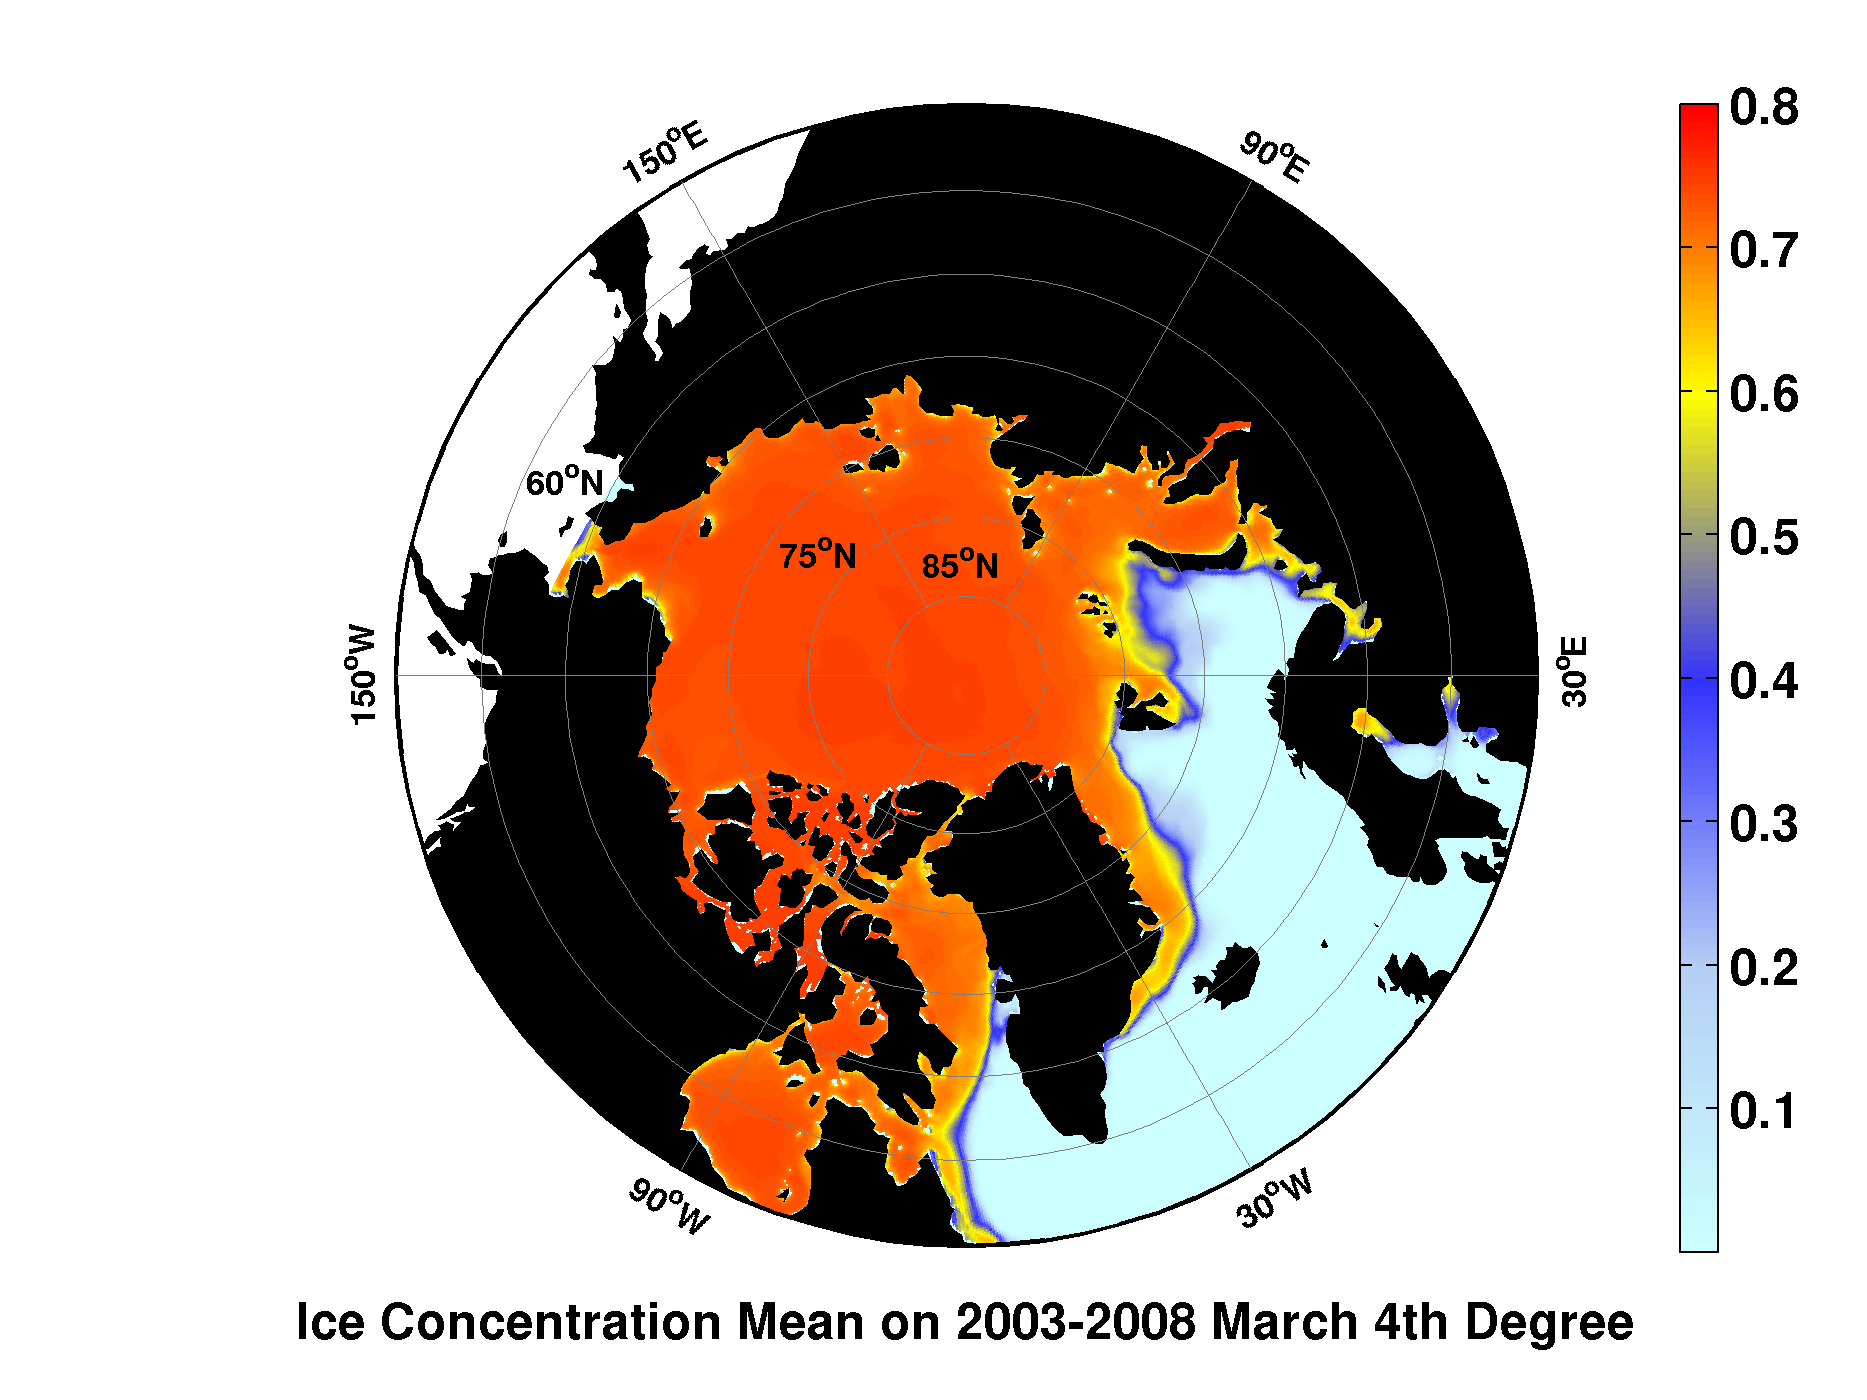
\includegraphics[width=\linewidth]{/home/jingfan/Desktop/Step1/1/Ice_Concentration_mean_2003-2008_March_4th_Degree.png}
\end{column}
\begin{column}[t]{0.5\linewidth}
\centering
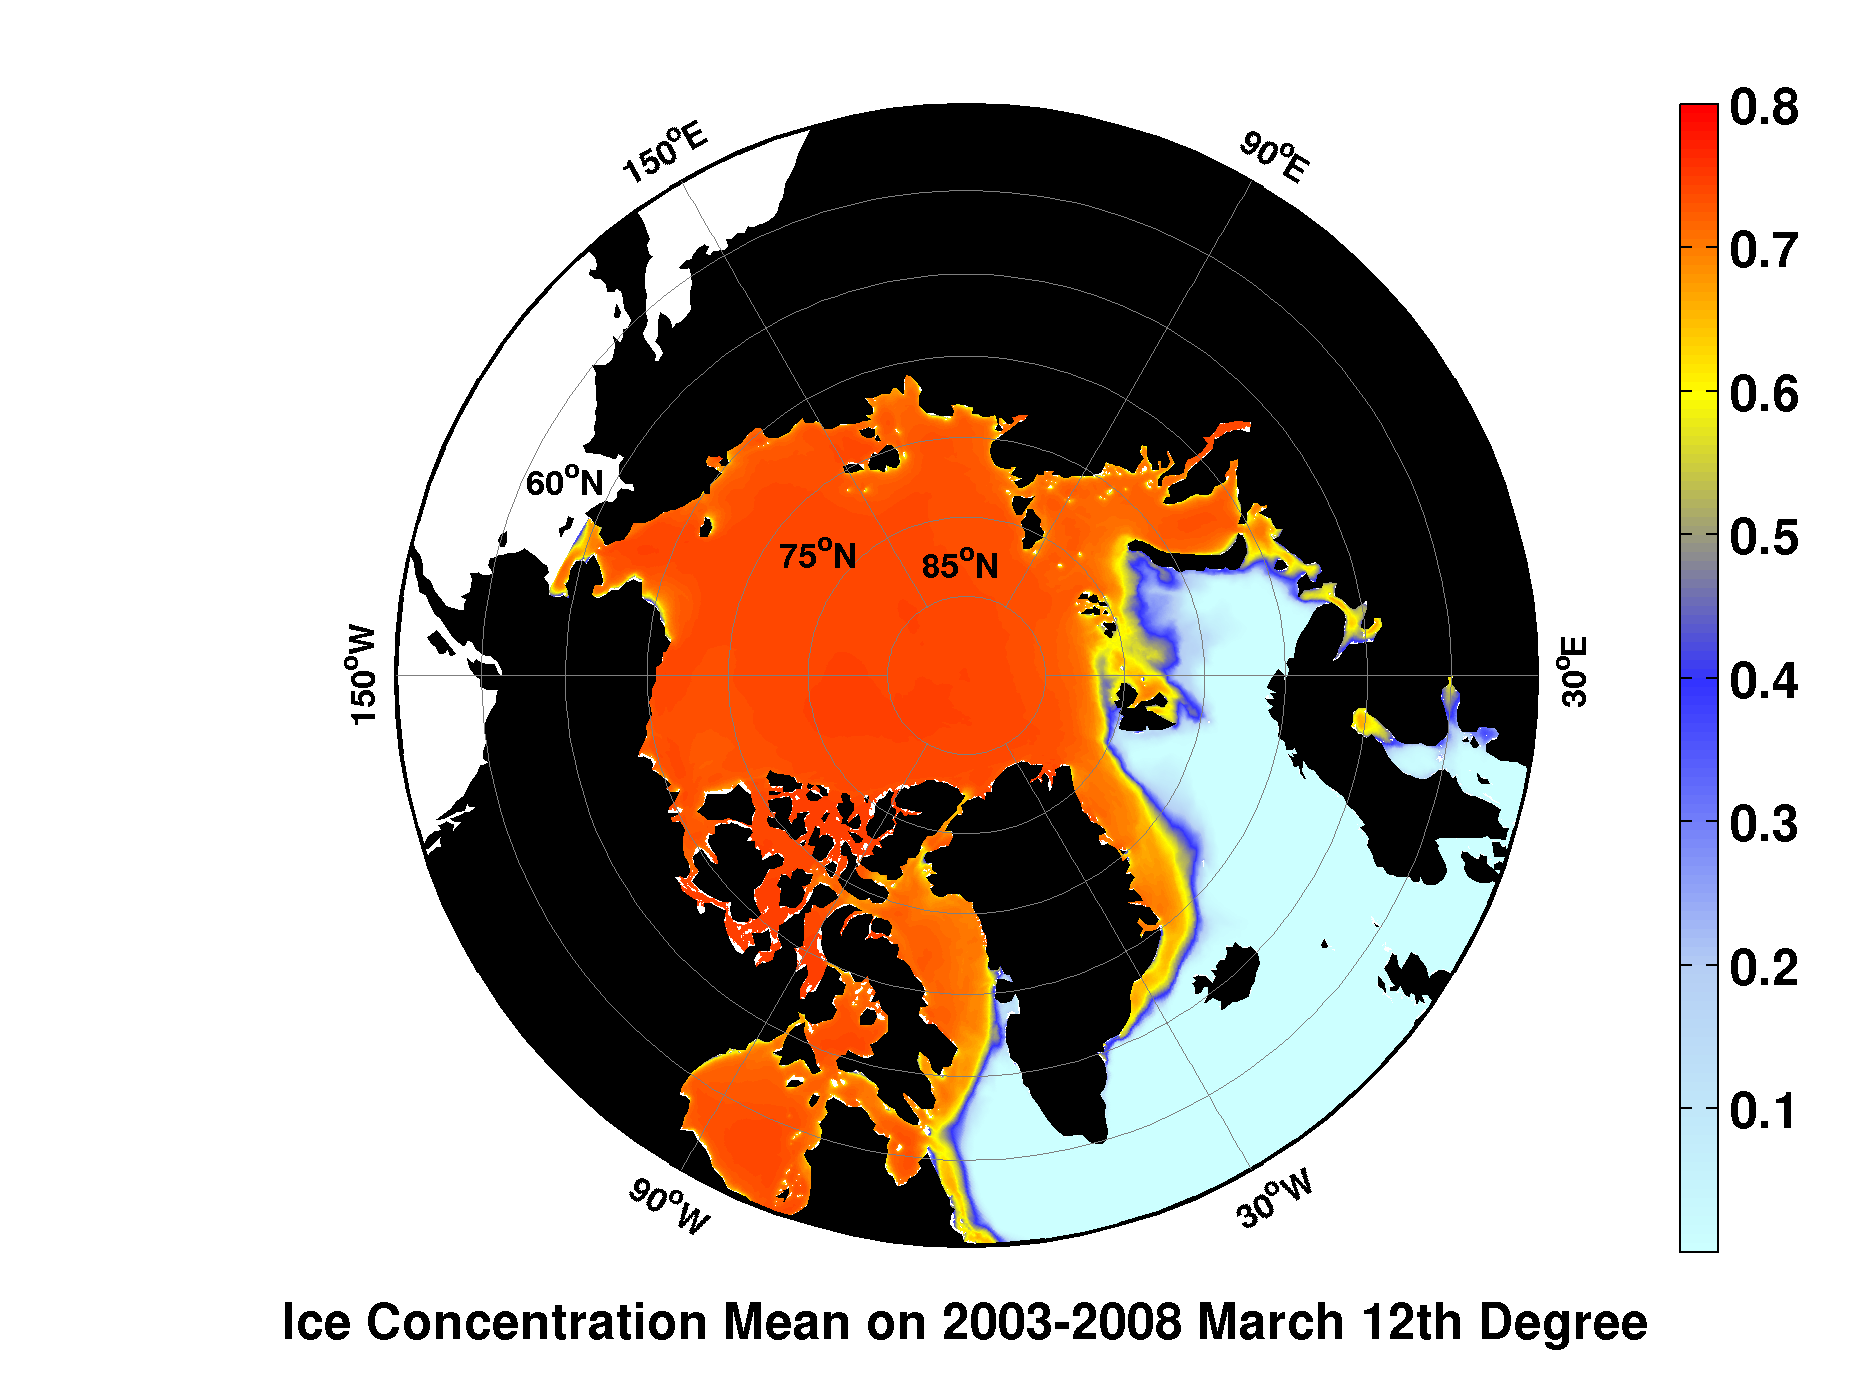
\includegraphics[width=\linewidth]{/home/jingfan/Desktop/Step1/1/Ice_Concentration_mean_2003-2008_March_12th_Degree.png}
\end{column}
\end{columns}

\end{frame}

\begin{frame}
\frametitle{Mean Sea-Ice Concentration Difference(ANHA12-ANHA4)}

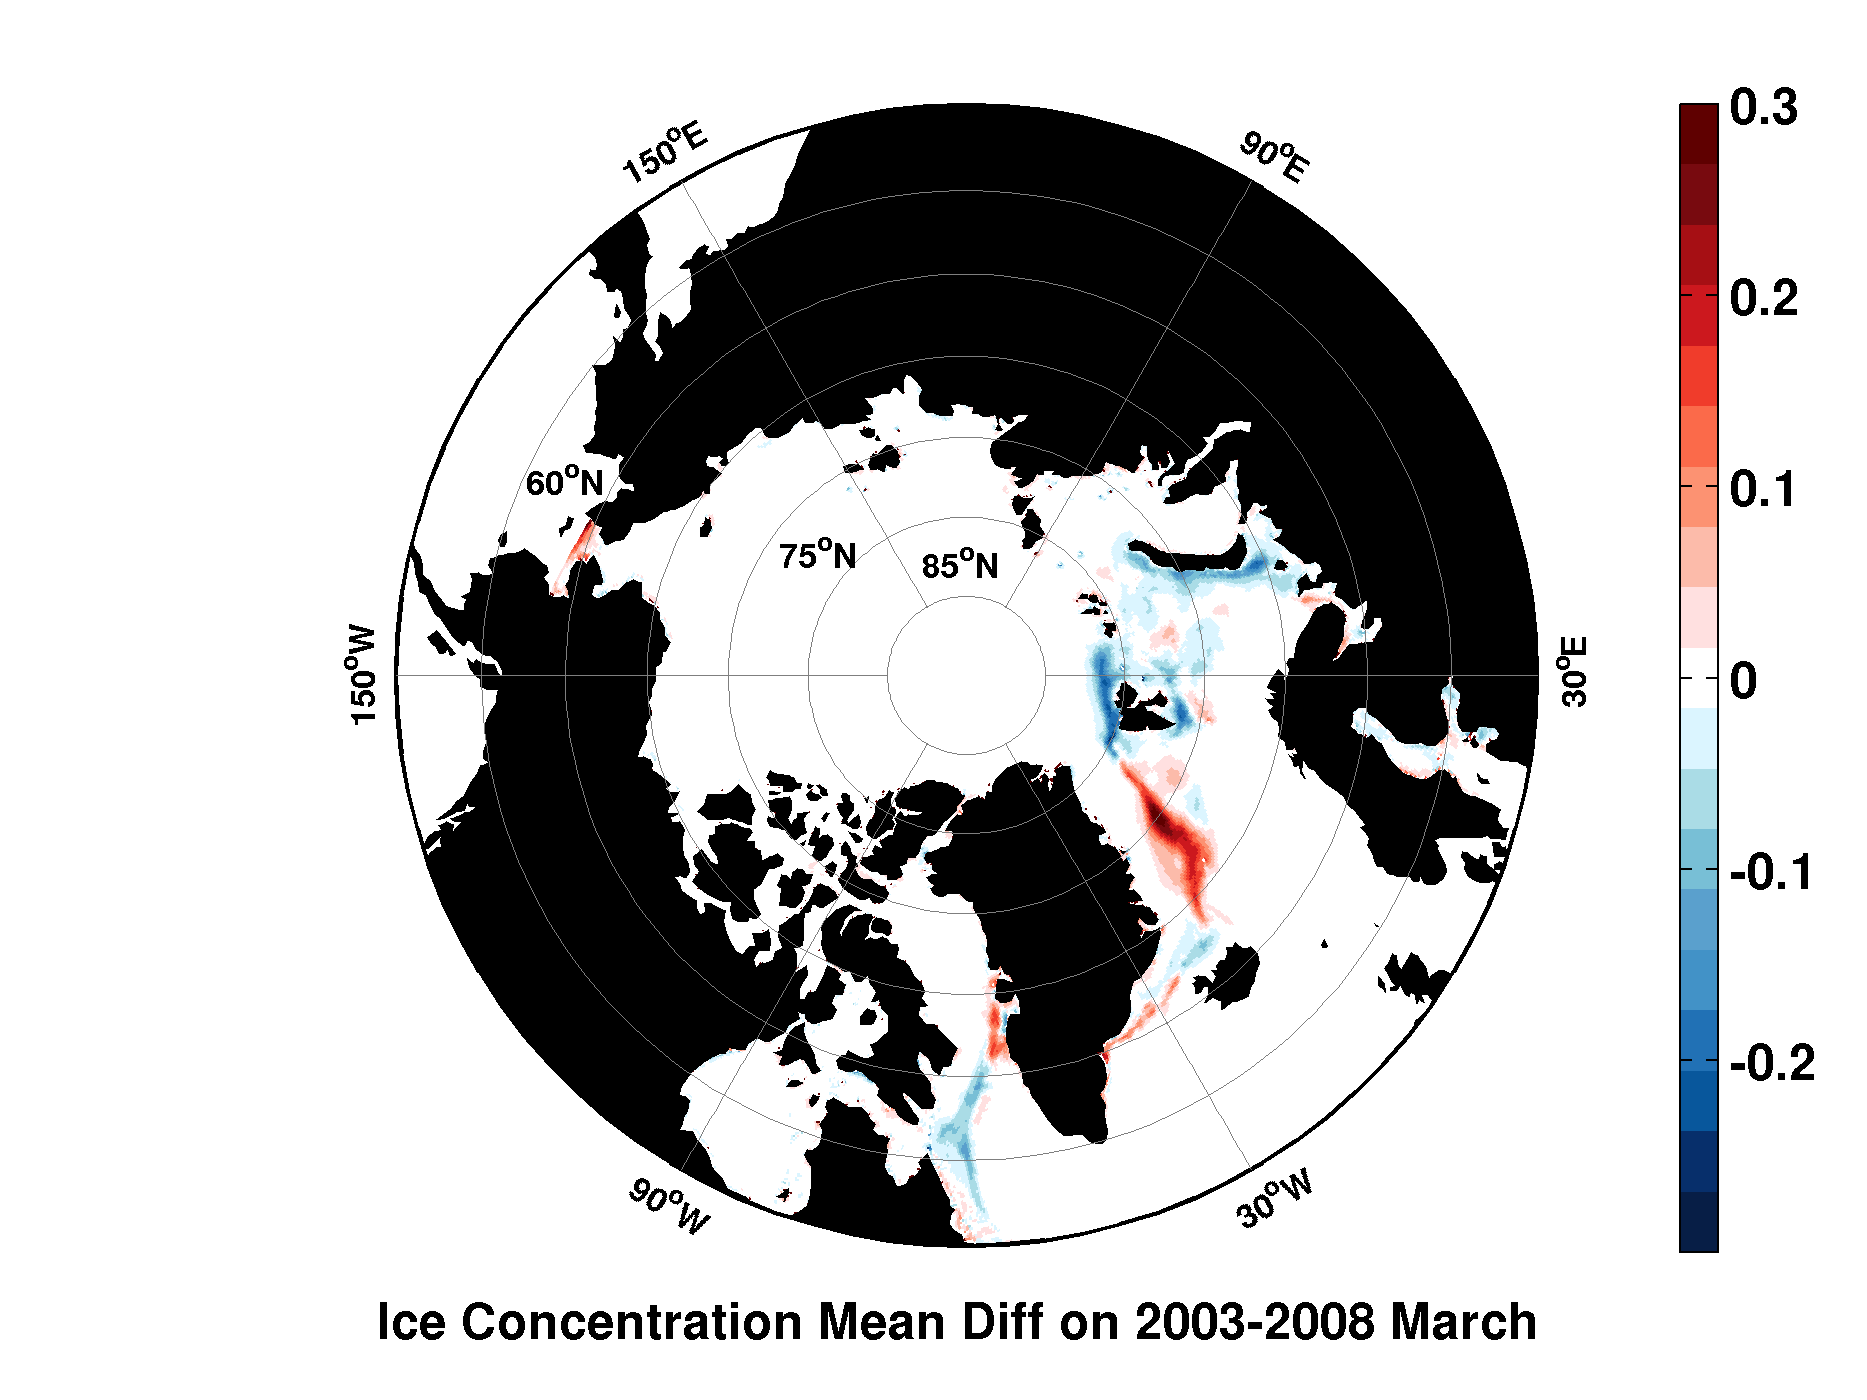
\includegraphics[width=0.9\linewidth]{/home/jingfan/Desktop/Step1/1/Ice_Concentration_mean_Diff_2003-2008_March.png}

\end{frame}

\begin{frame}
\frametitle{Mean Sea-Ice Concentration}

\begin{columns}
\begin{column}[t]{0.5\linewidth}
\centering
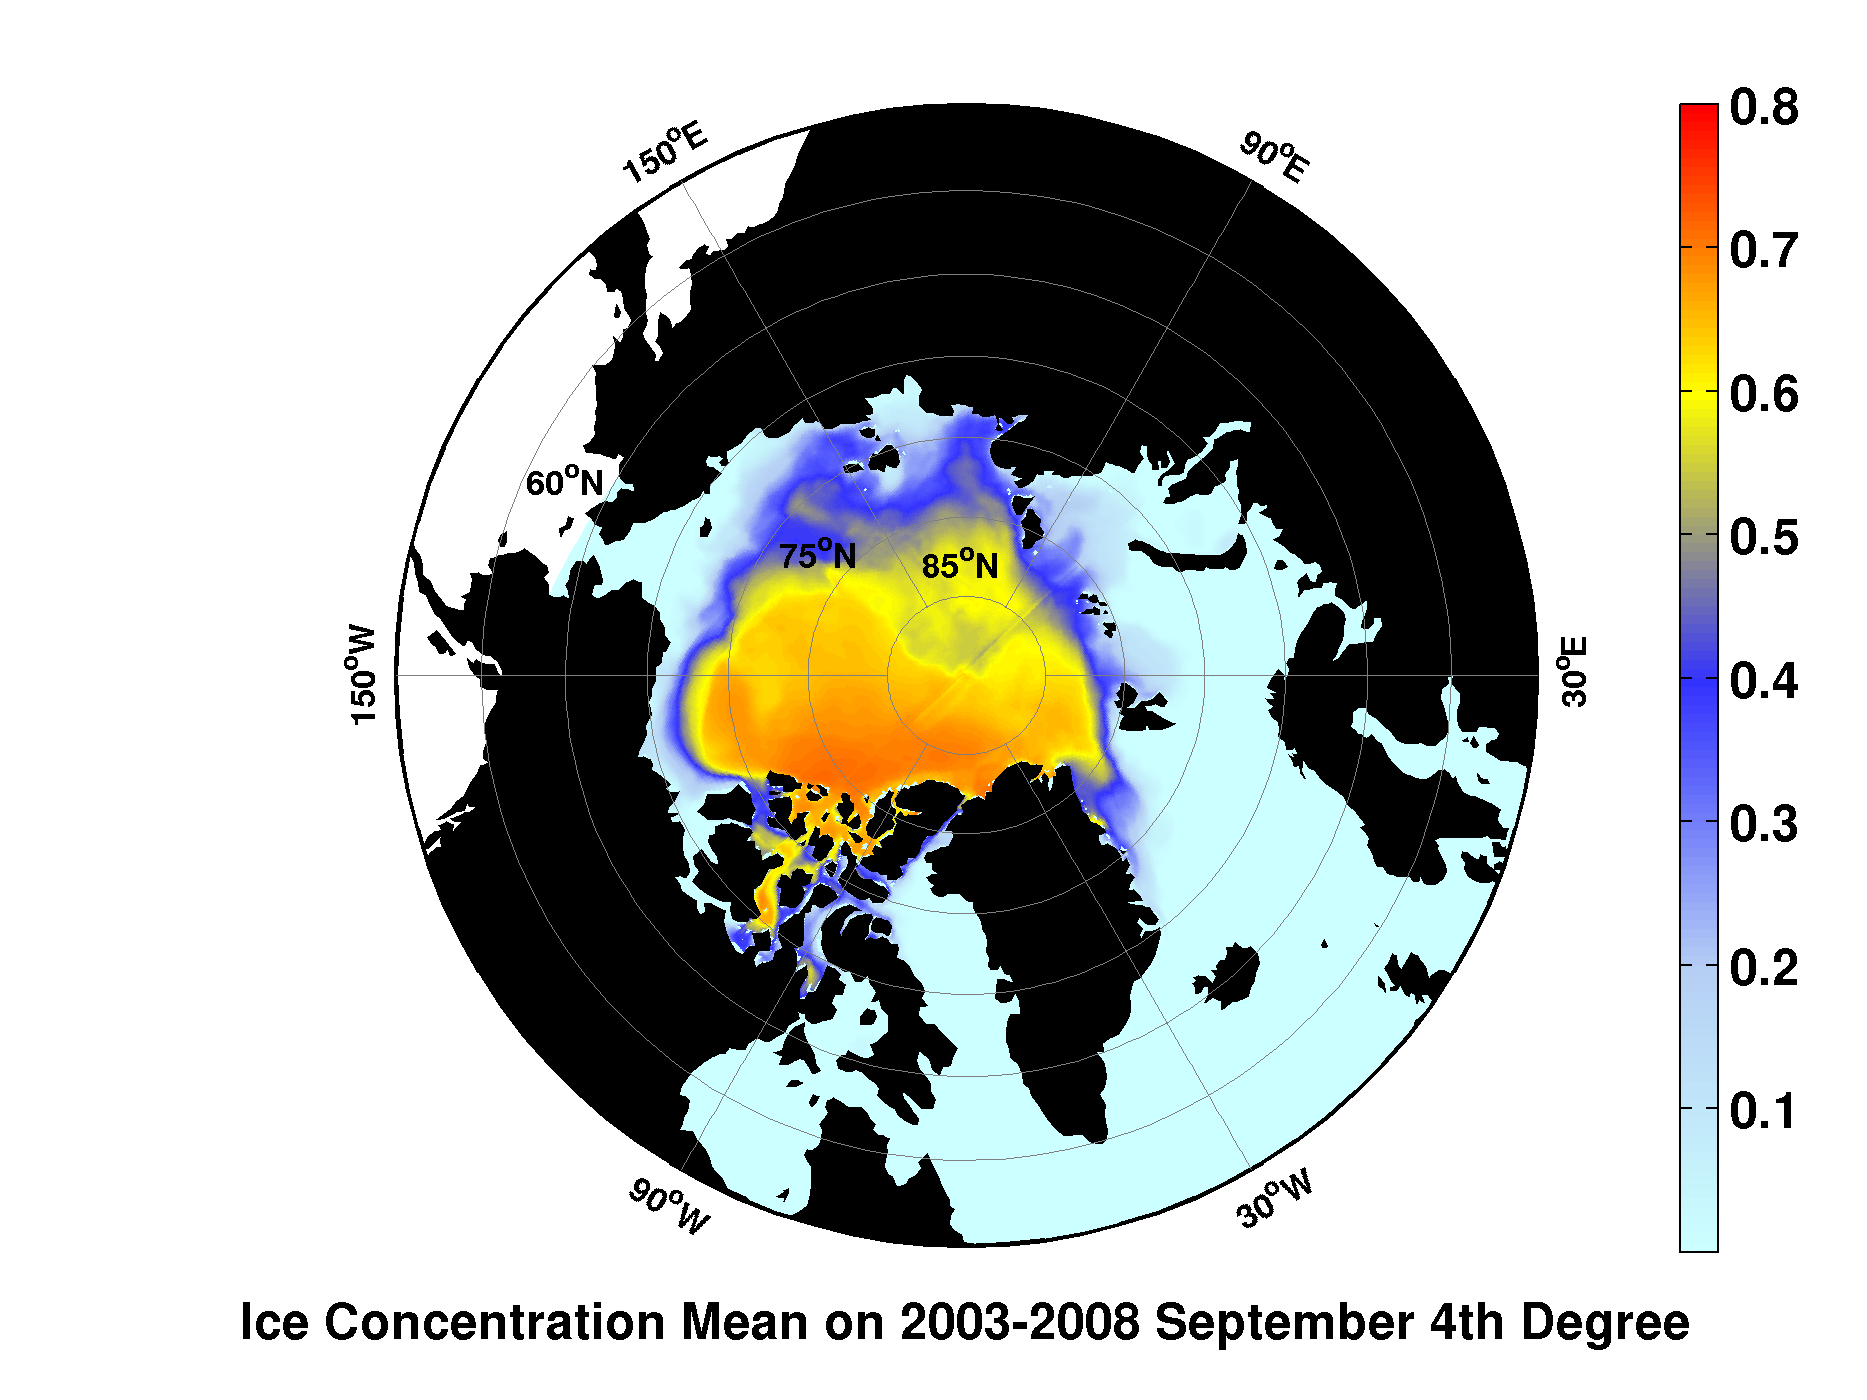
\includegraphics[width=\linewidth]{/home/jingfan/Desktop/Step1/1/Ice_Concentration_mean_2003-2008_September_4th_Degree.png}
\end{column}
\begin{column}[t]{0.5\linewidth}
\centering
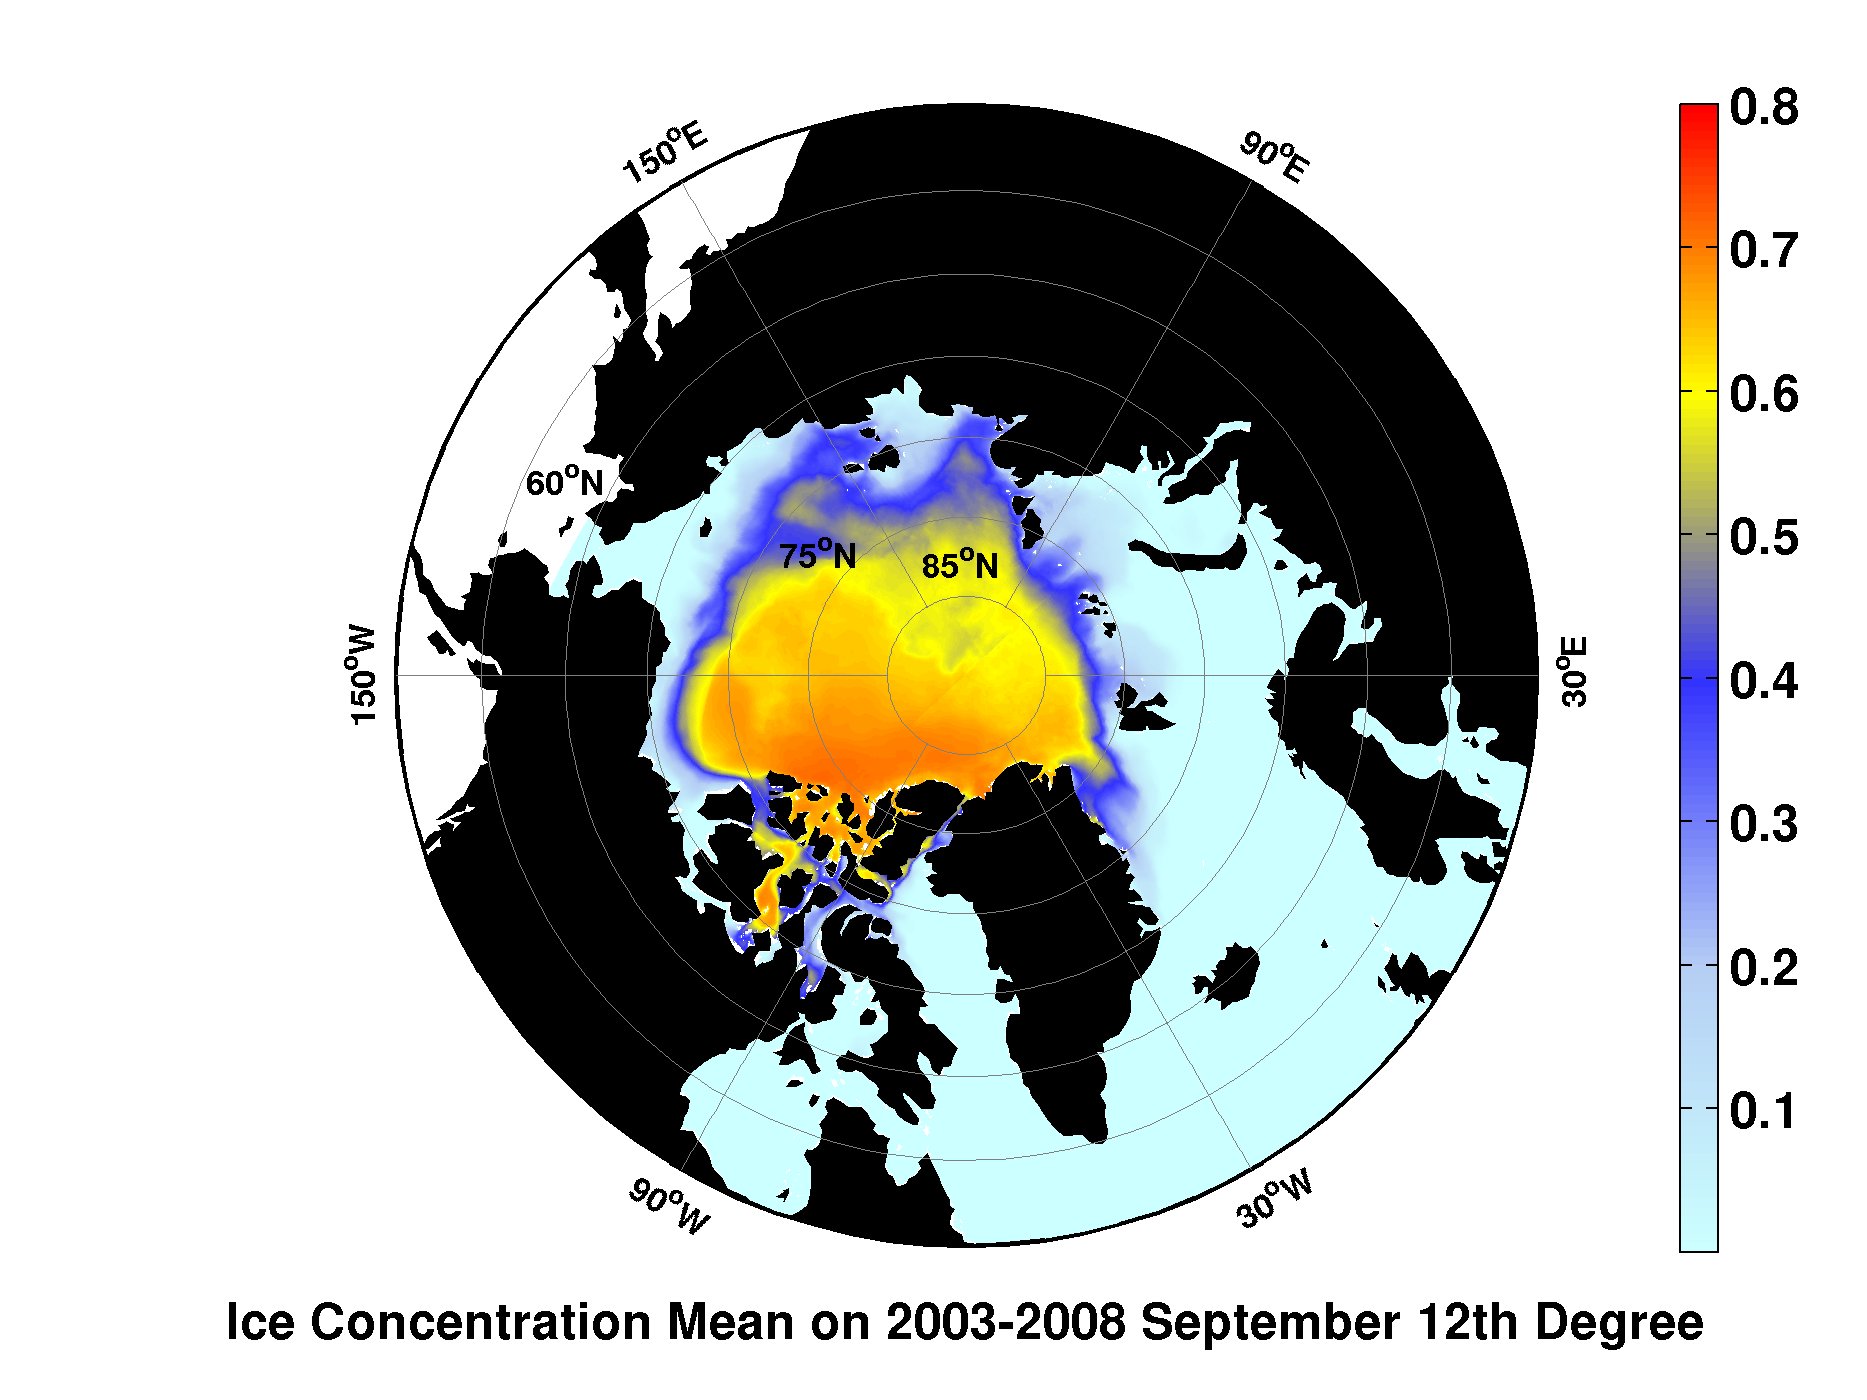
\includegraphics[width=\linewidth]{/home/jingfan/Desktop/Step1/1/Ice_Concentration_mean_2003-2008_September_12th_Degree.png}
\end{column}
\end{columns}

\end{frame}

\begin{frame}
\frametitle{Mean Sea-Ice Concentration Difference(ANHA12-ANHA4)}

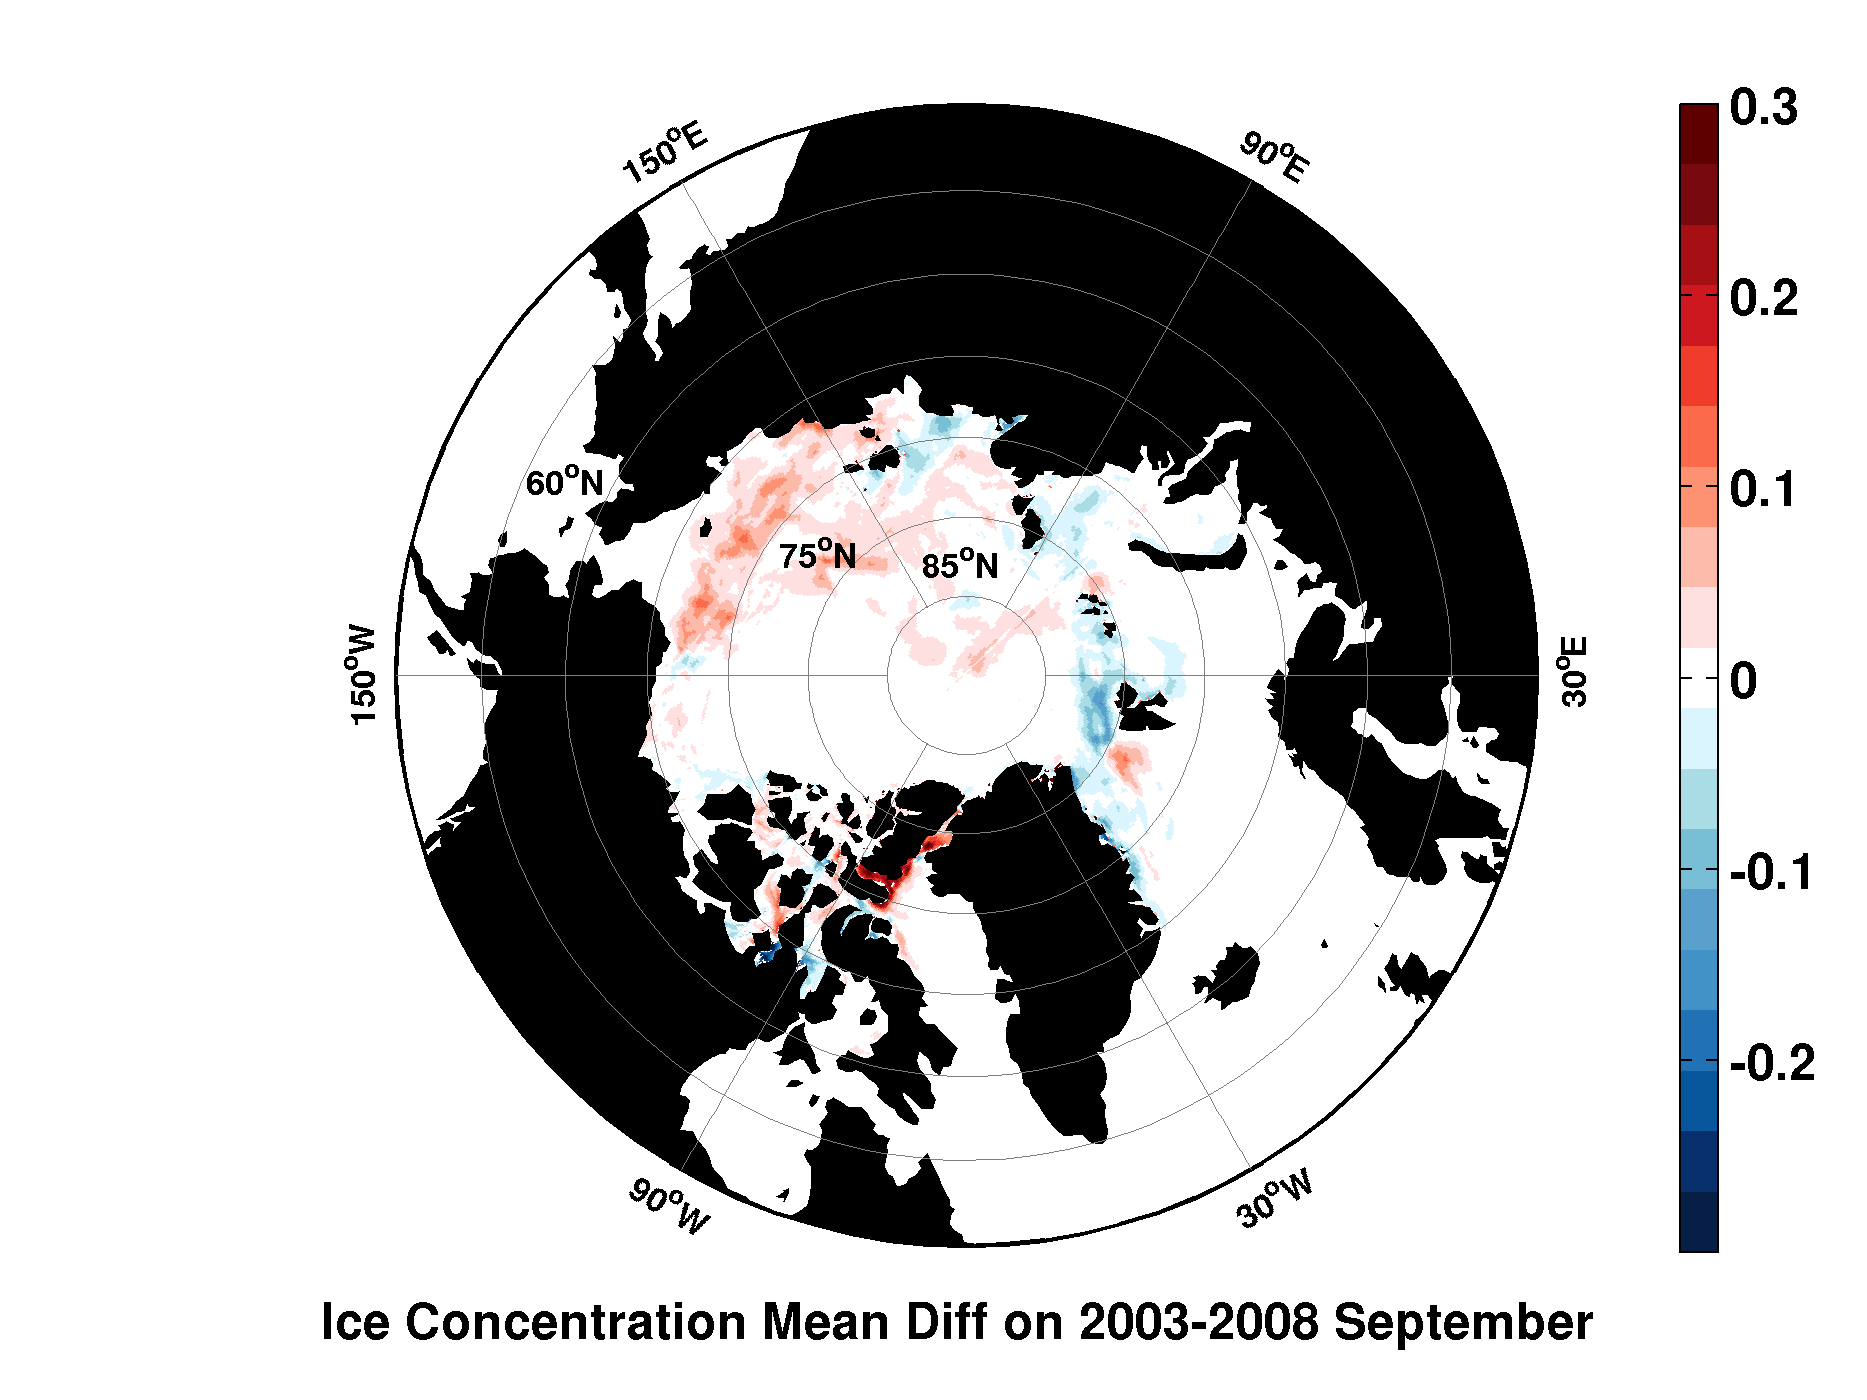
\includegraphics[width=0.9\linewidth]{/home/jingfan/Desktop/Step1/1/Ice_Concentration_mean_Diff_2003-2008_September.png}

\end{frame}

%%%%%%%%%%%%%%%%%%%%%%%%%%%%%%%%%%%%%%%%%%%%%%%%%%%%%%%%%%%%%
\begin{frame}
\frametitle{Sea-Ice Concentration Standard Deviation}
I calculate the standard deviation on each grid point from 2003-2008 with following equation: $$ STD = \sqrt{\frac{1}{N-1}\sum^N_{i=1}(x_i-\mu)^2} $$
The sample for each grid point is a vector of 6 numbers.
\end{frame}

\begin{frame}
\frametitle{Sea-Ice Concentration Standard Deviation}

\begin{columns}
\begin{column}[t]{0.5\linewidth}
\centering
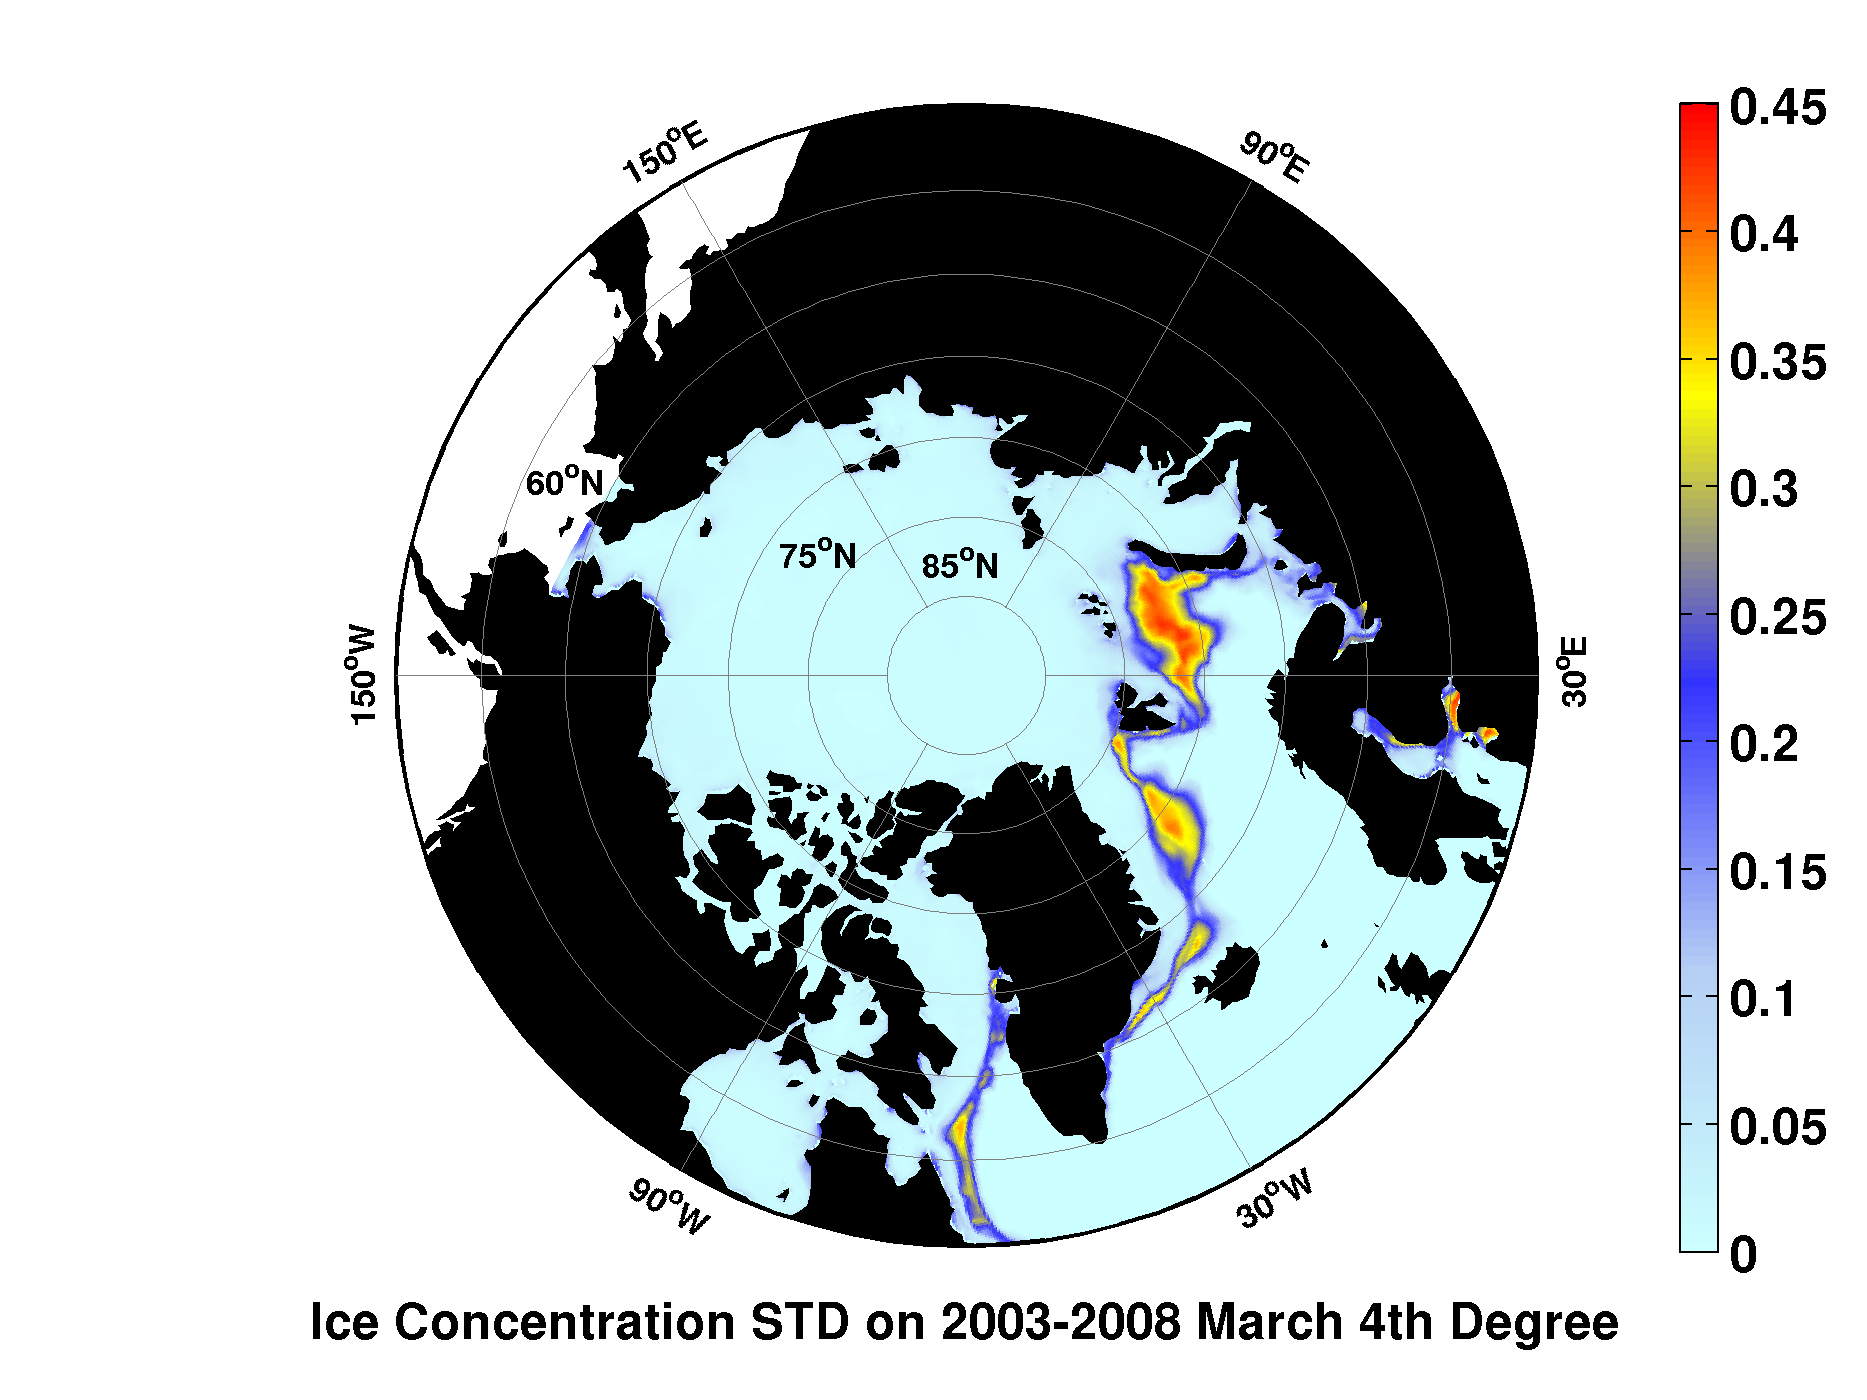
\includegraphics[width=\linewidth]{/home/jingfan/Desktop/Step1/2/Ice_Cocnentration_STD_2003-2008_March_4th_Degree.png}
\end{column}
\begin{column}[t]{0.5\linewidth}
\centering
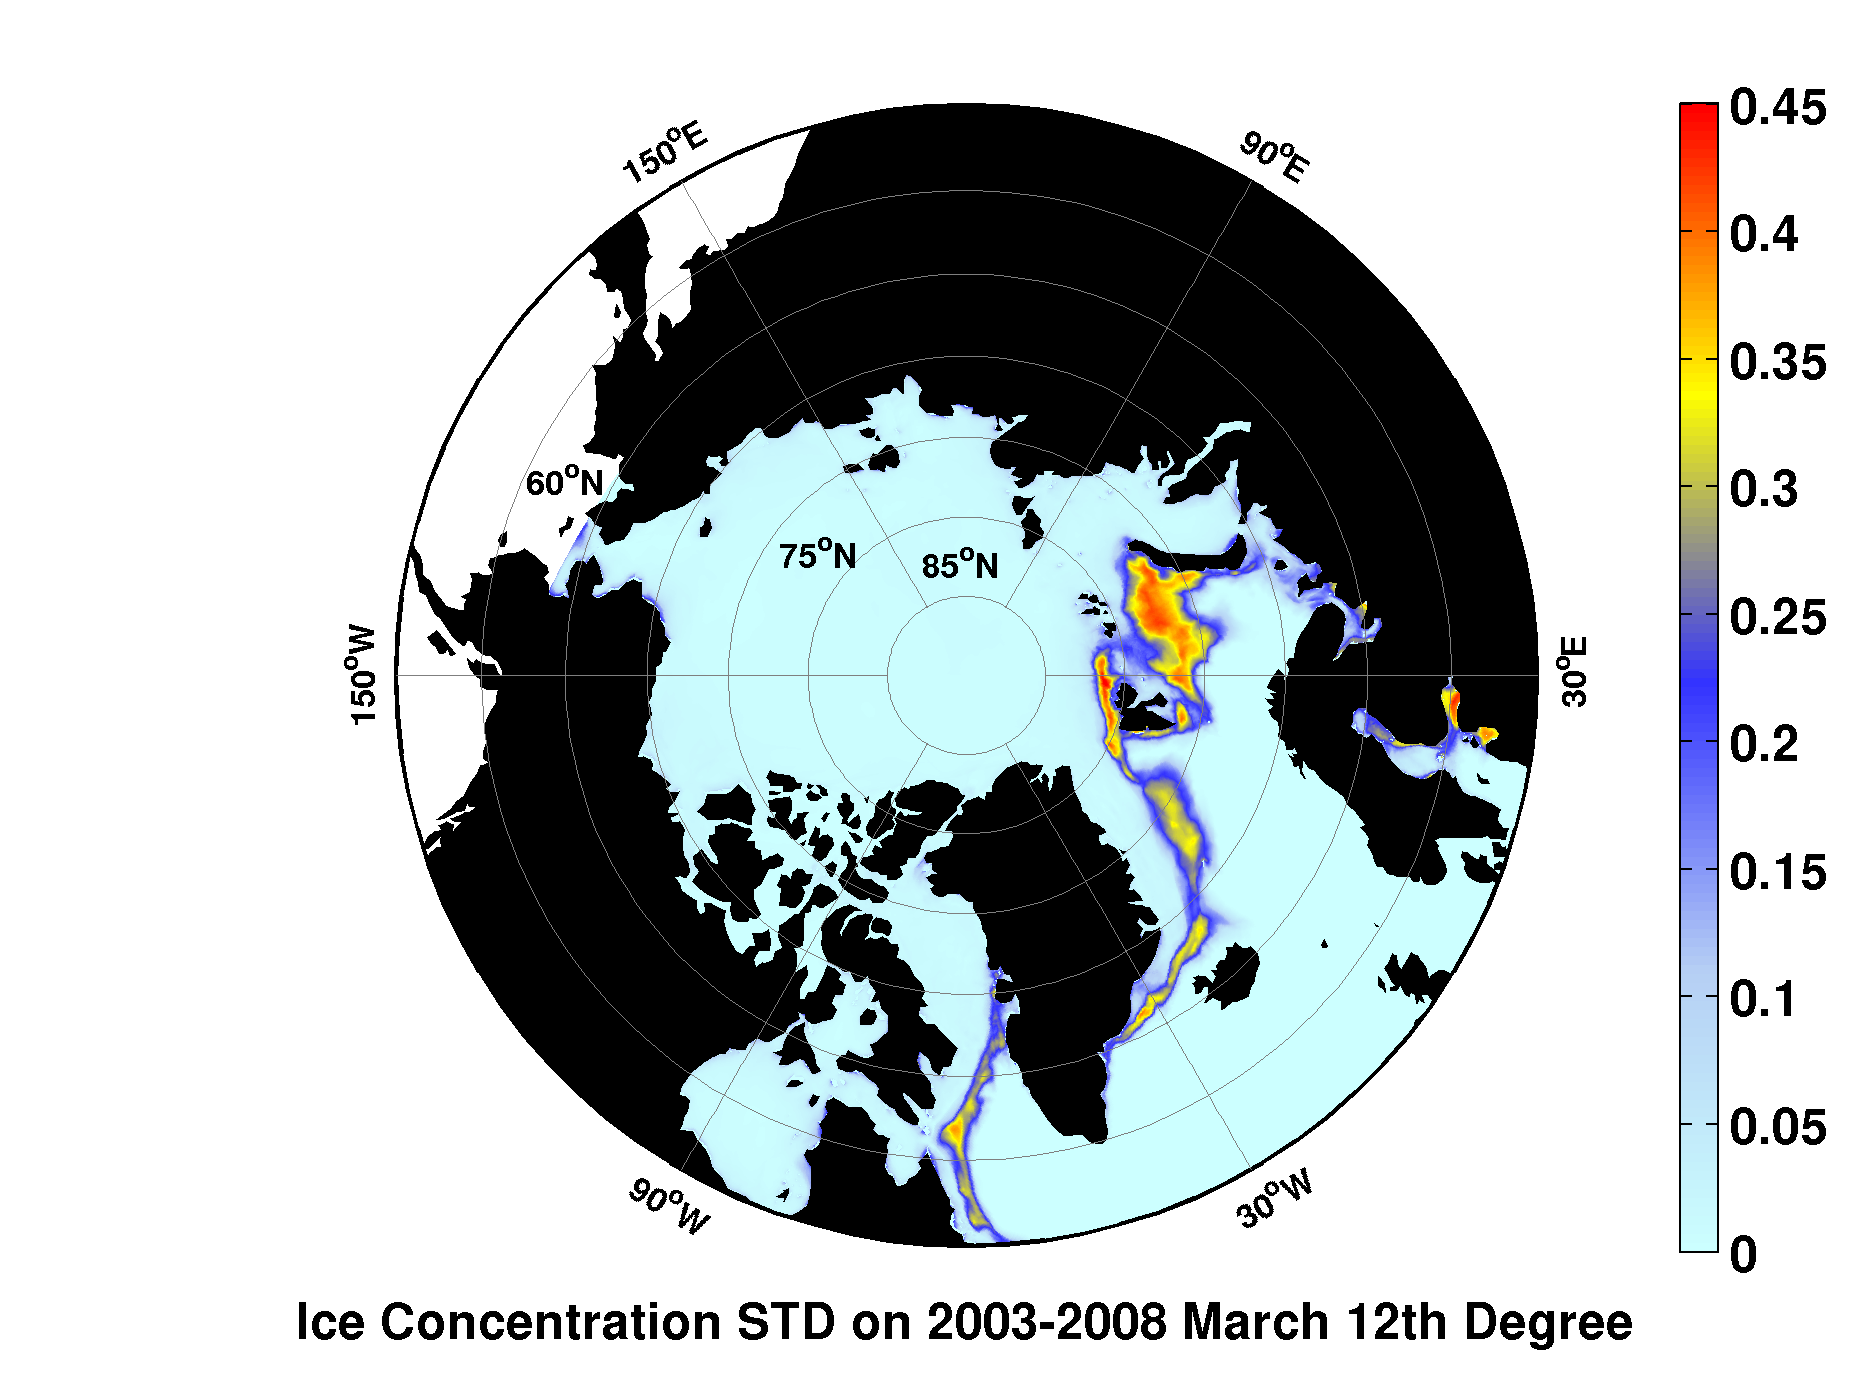
\includegraphics[width=\linewidth]{/home/jingfan/Desktop/Step1/2/Ice_Concentration_STD_2003-2008_March_12th_Degree.png}
\end{column}
\end{columns}

\end{frame}

\begin{frame}
\frametitle{Sea-Ice Concentration Standard Deviation Difference(ANHA12-ANHA4)}

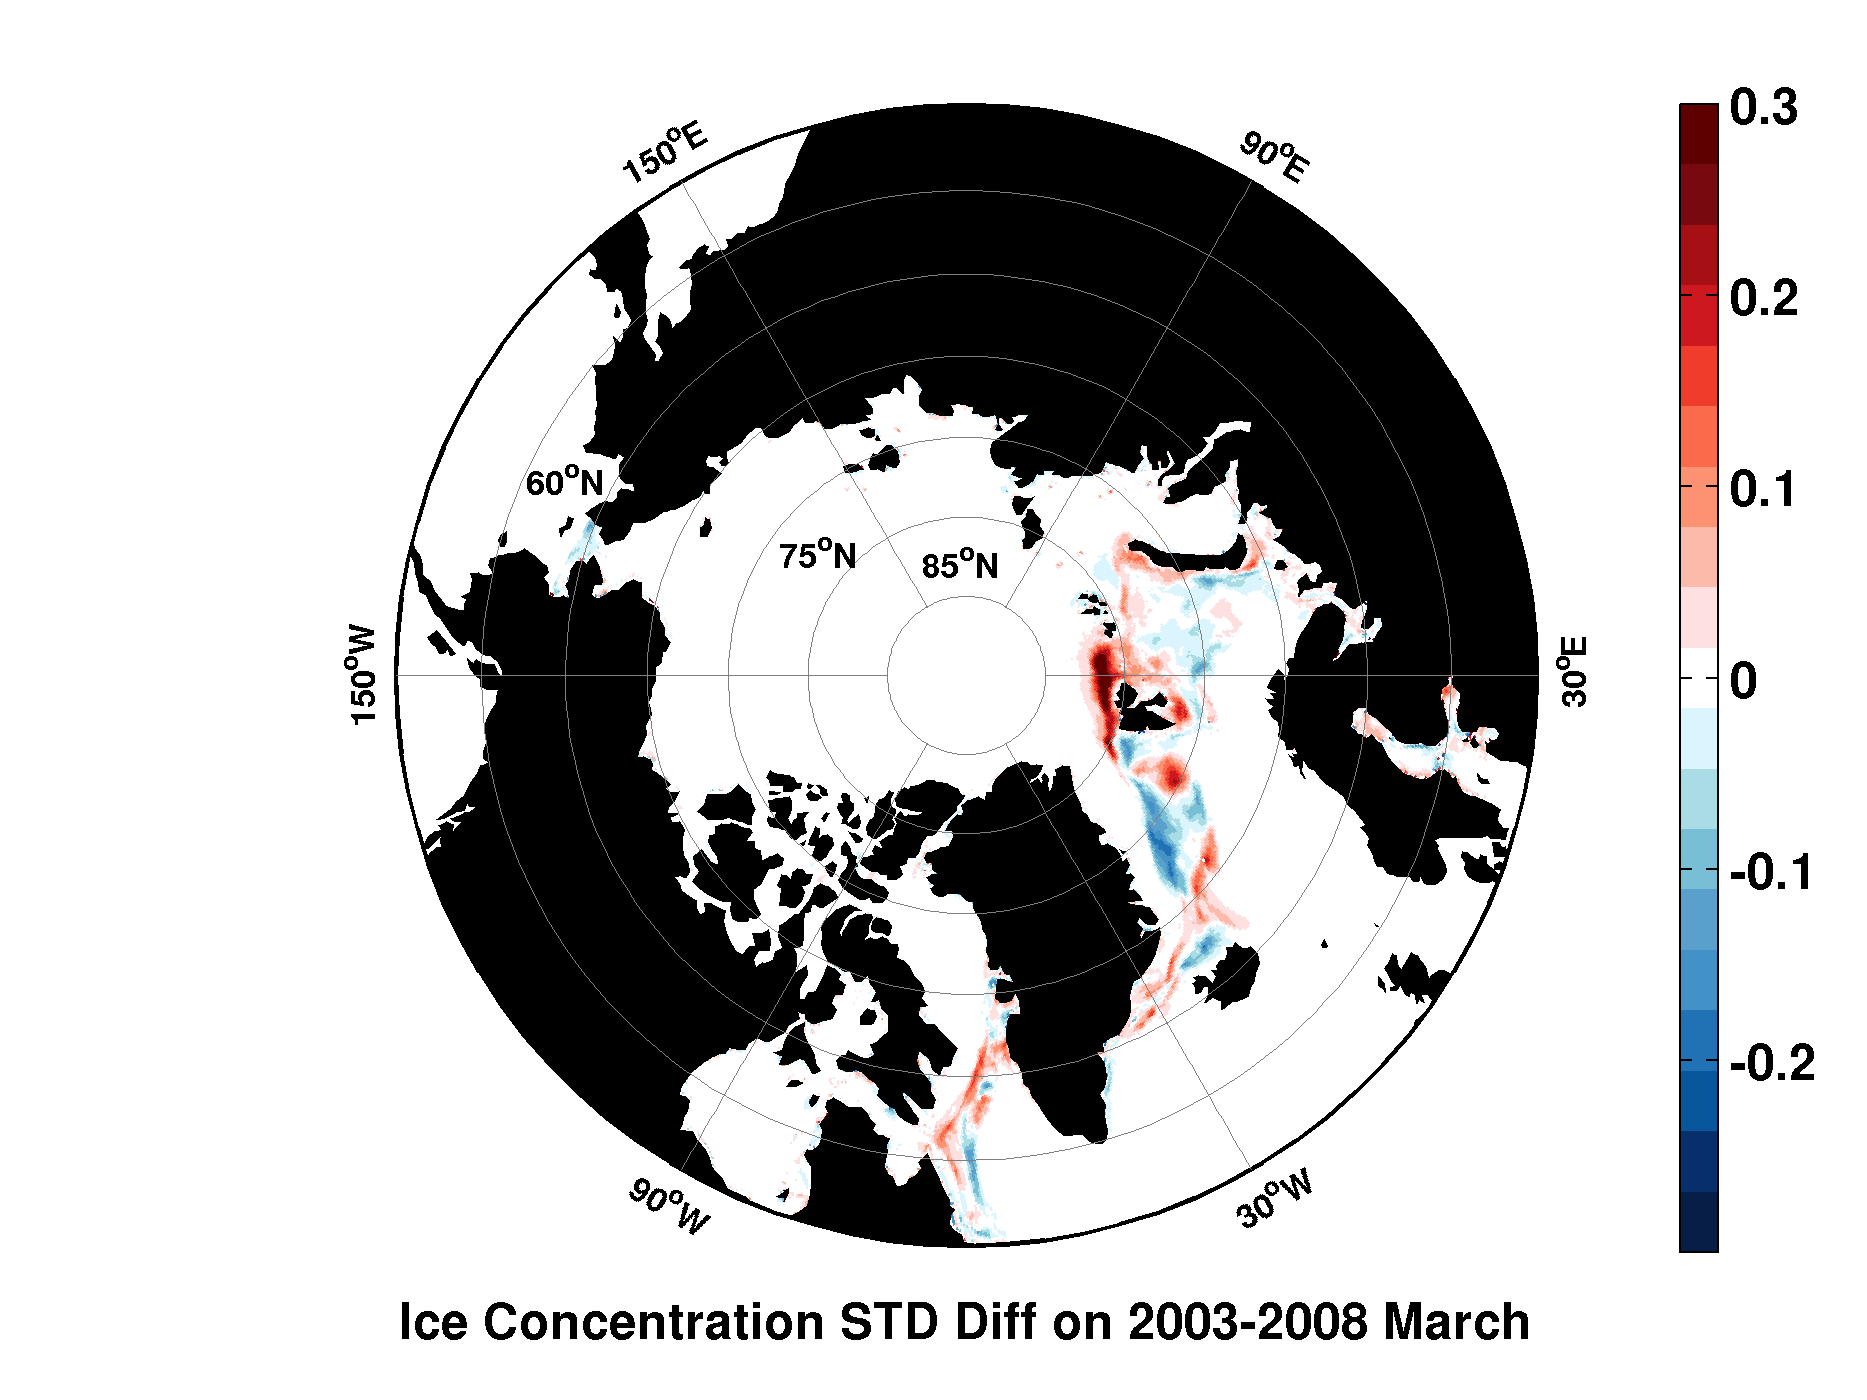
\includegraphics[width=0.9\linewidth]{/home/jingfan/Desktop/Step1/2/Ice_Concentration_STD_Diff_2003-2008_March.png}

\end{frame}

\begin{frame}
\frametitle{Sea-Ice Concentration Standard Deviation}

\begin{columns}
\begin{column}[t]{0.5\linewidth}
\centering
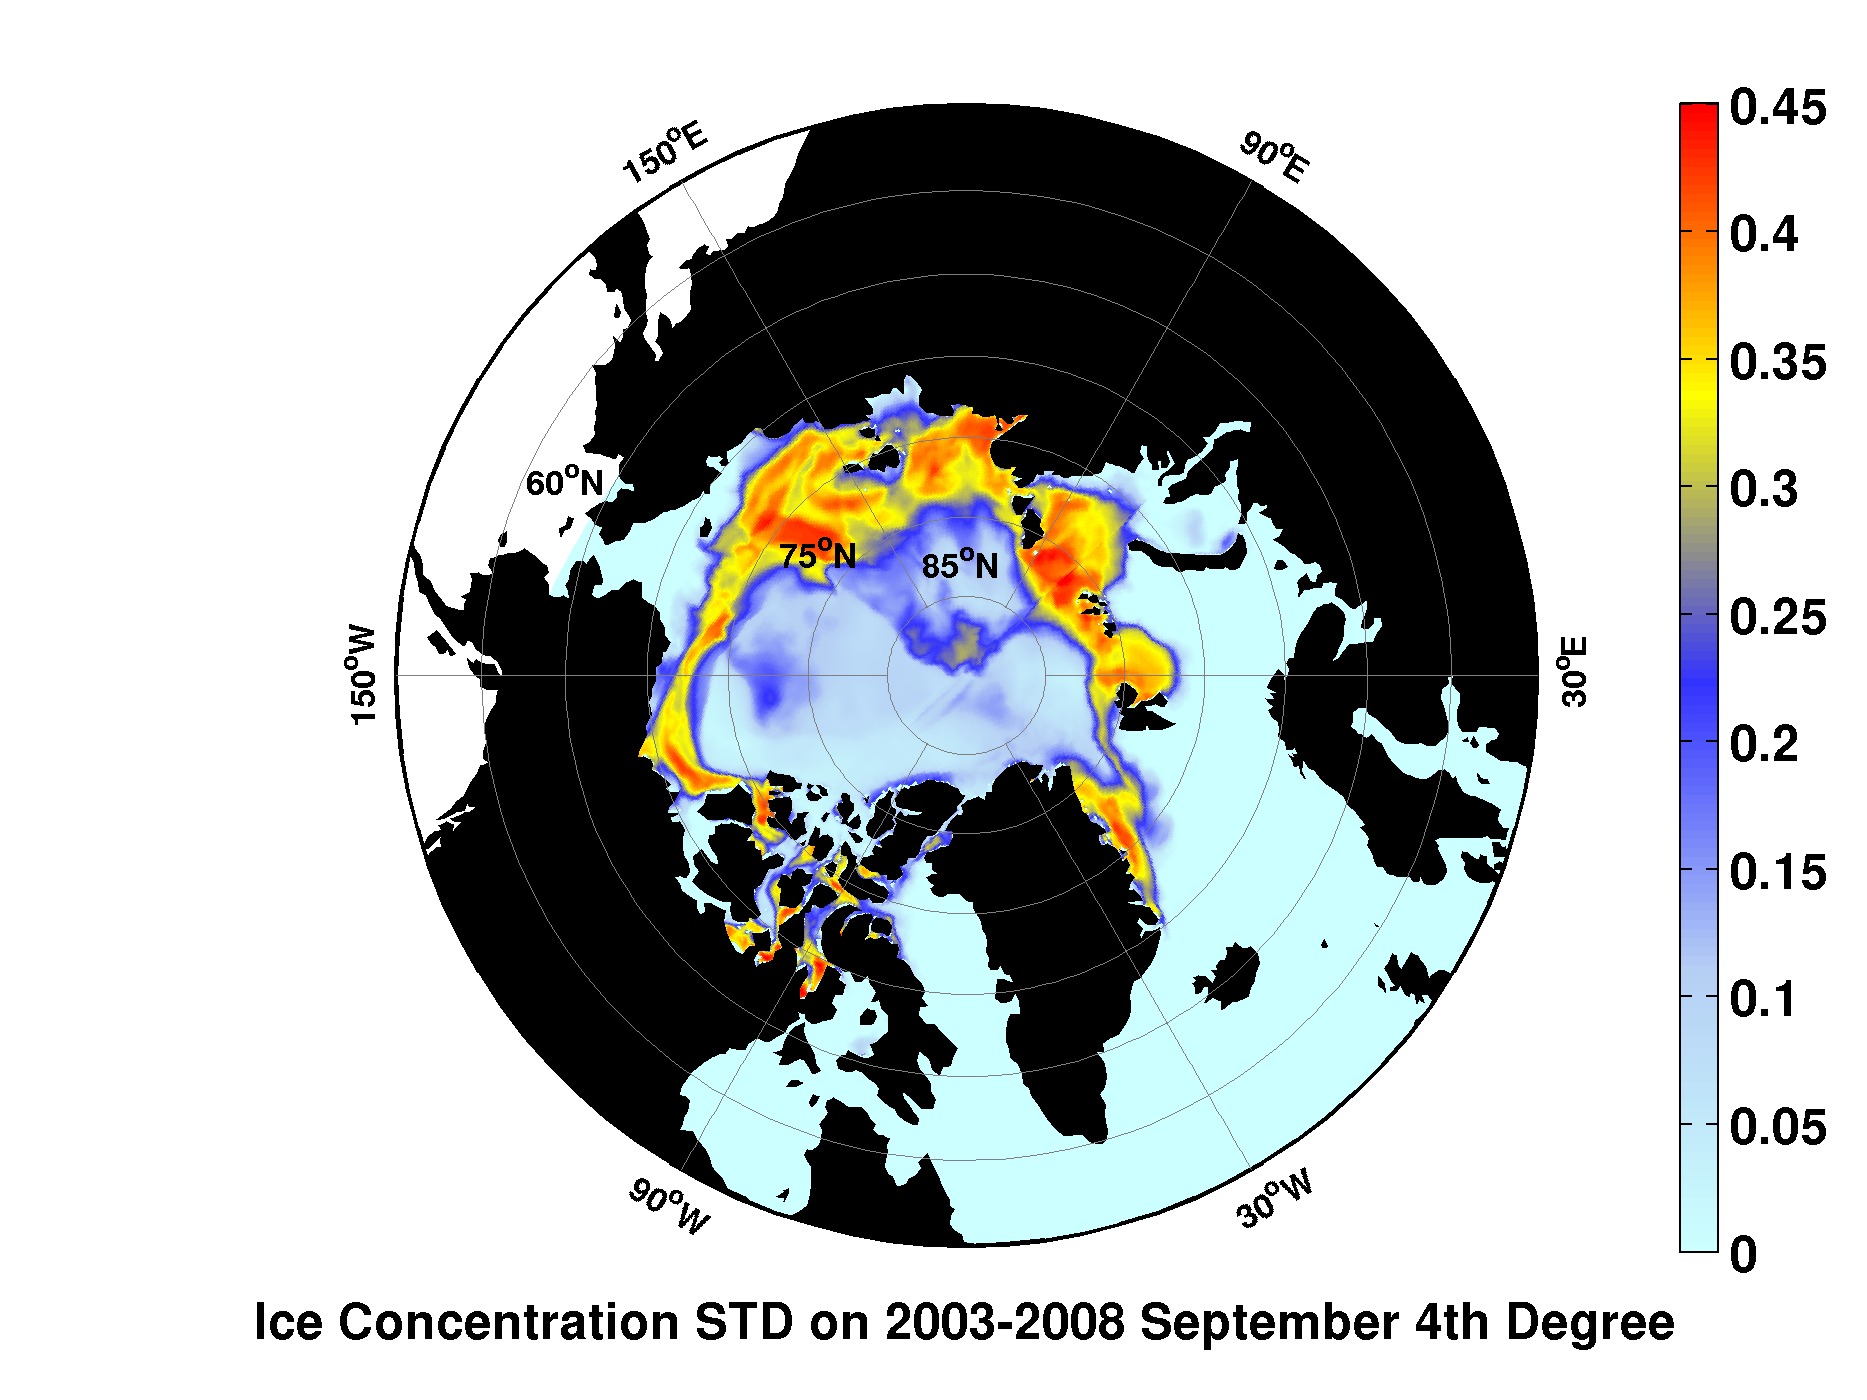
\includegraphics[width=\linewidth]{/home/jingfan/Desktop/Step1/2/Ice_Cocnentration_STD_2003-2008_September_4th_Degree.png}
\end{column}
\begin{column}[t]{0.5\linewidth}
\centering
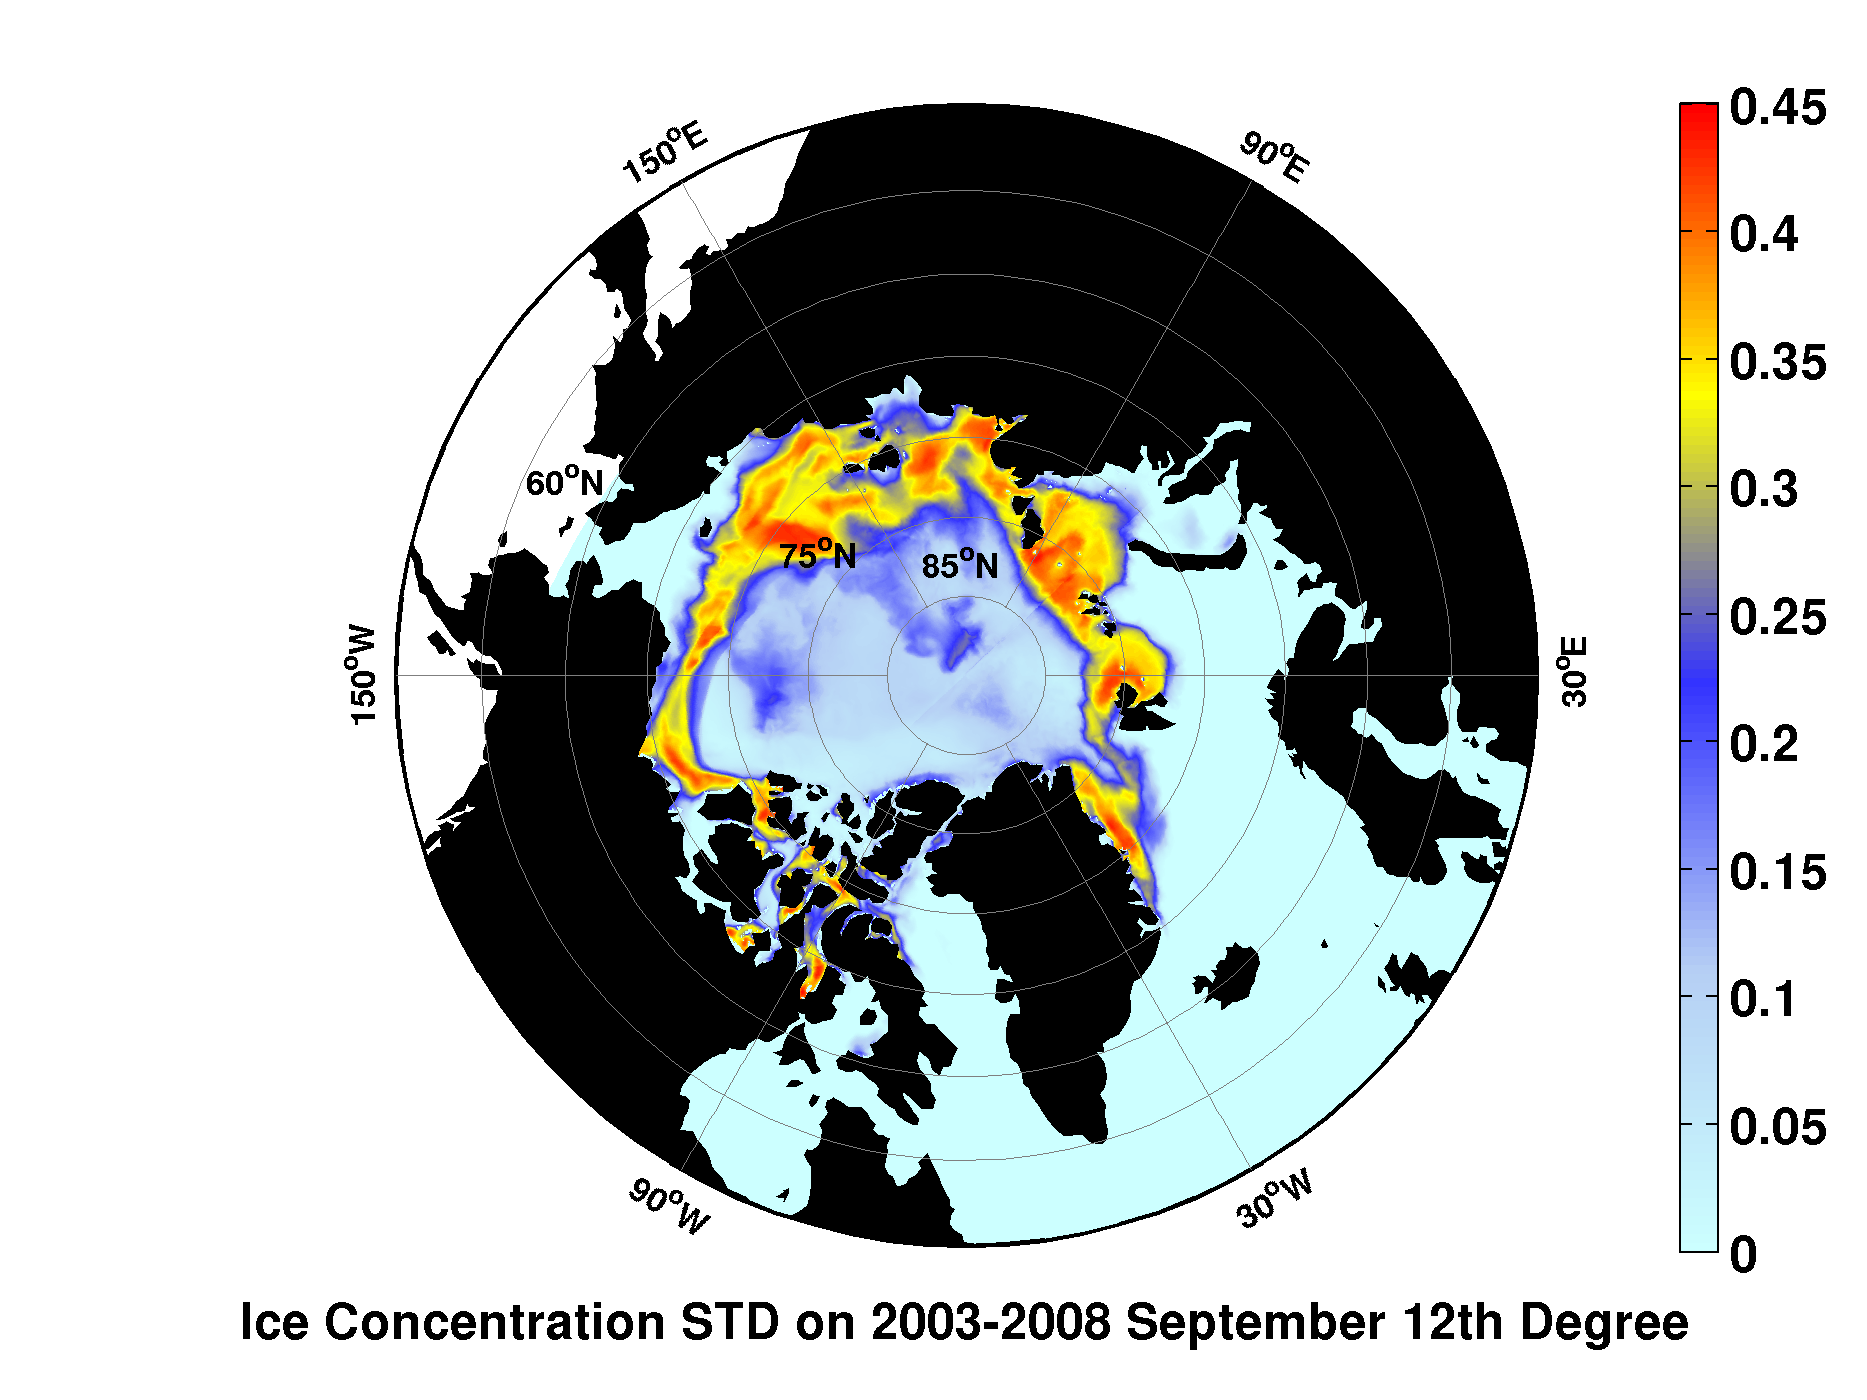
\includegraphics[width=\linewidth]{/home/jingfan/Desktop/Step1/2/Ice_Concentration_STD_2003-2008_September_12th_Degree.png}
\end{column}
\end{columns}

\end{frame}

\begin{frame}
\frametitle{Sea-Ice Concentration Standard Deviation Difference(ANHA12-ANHA4)}

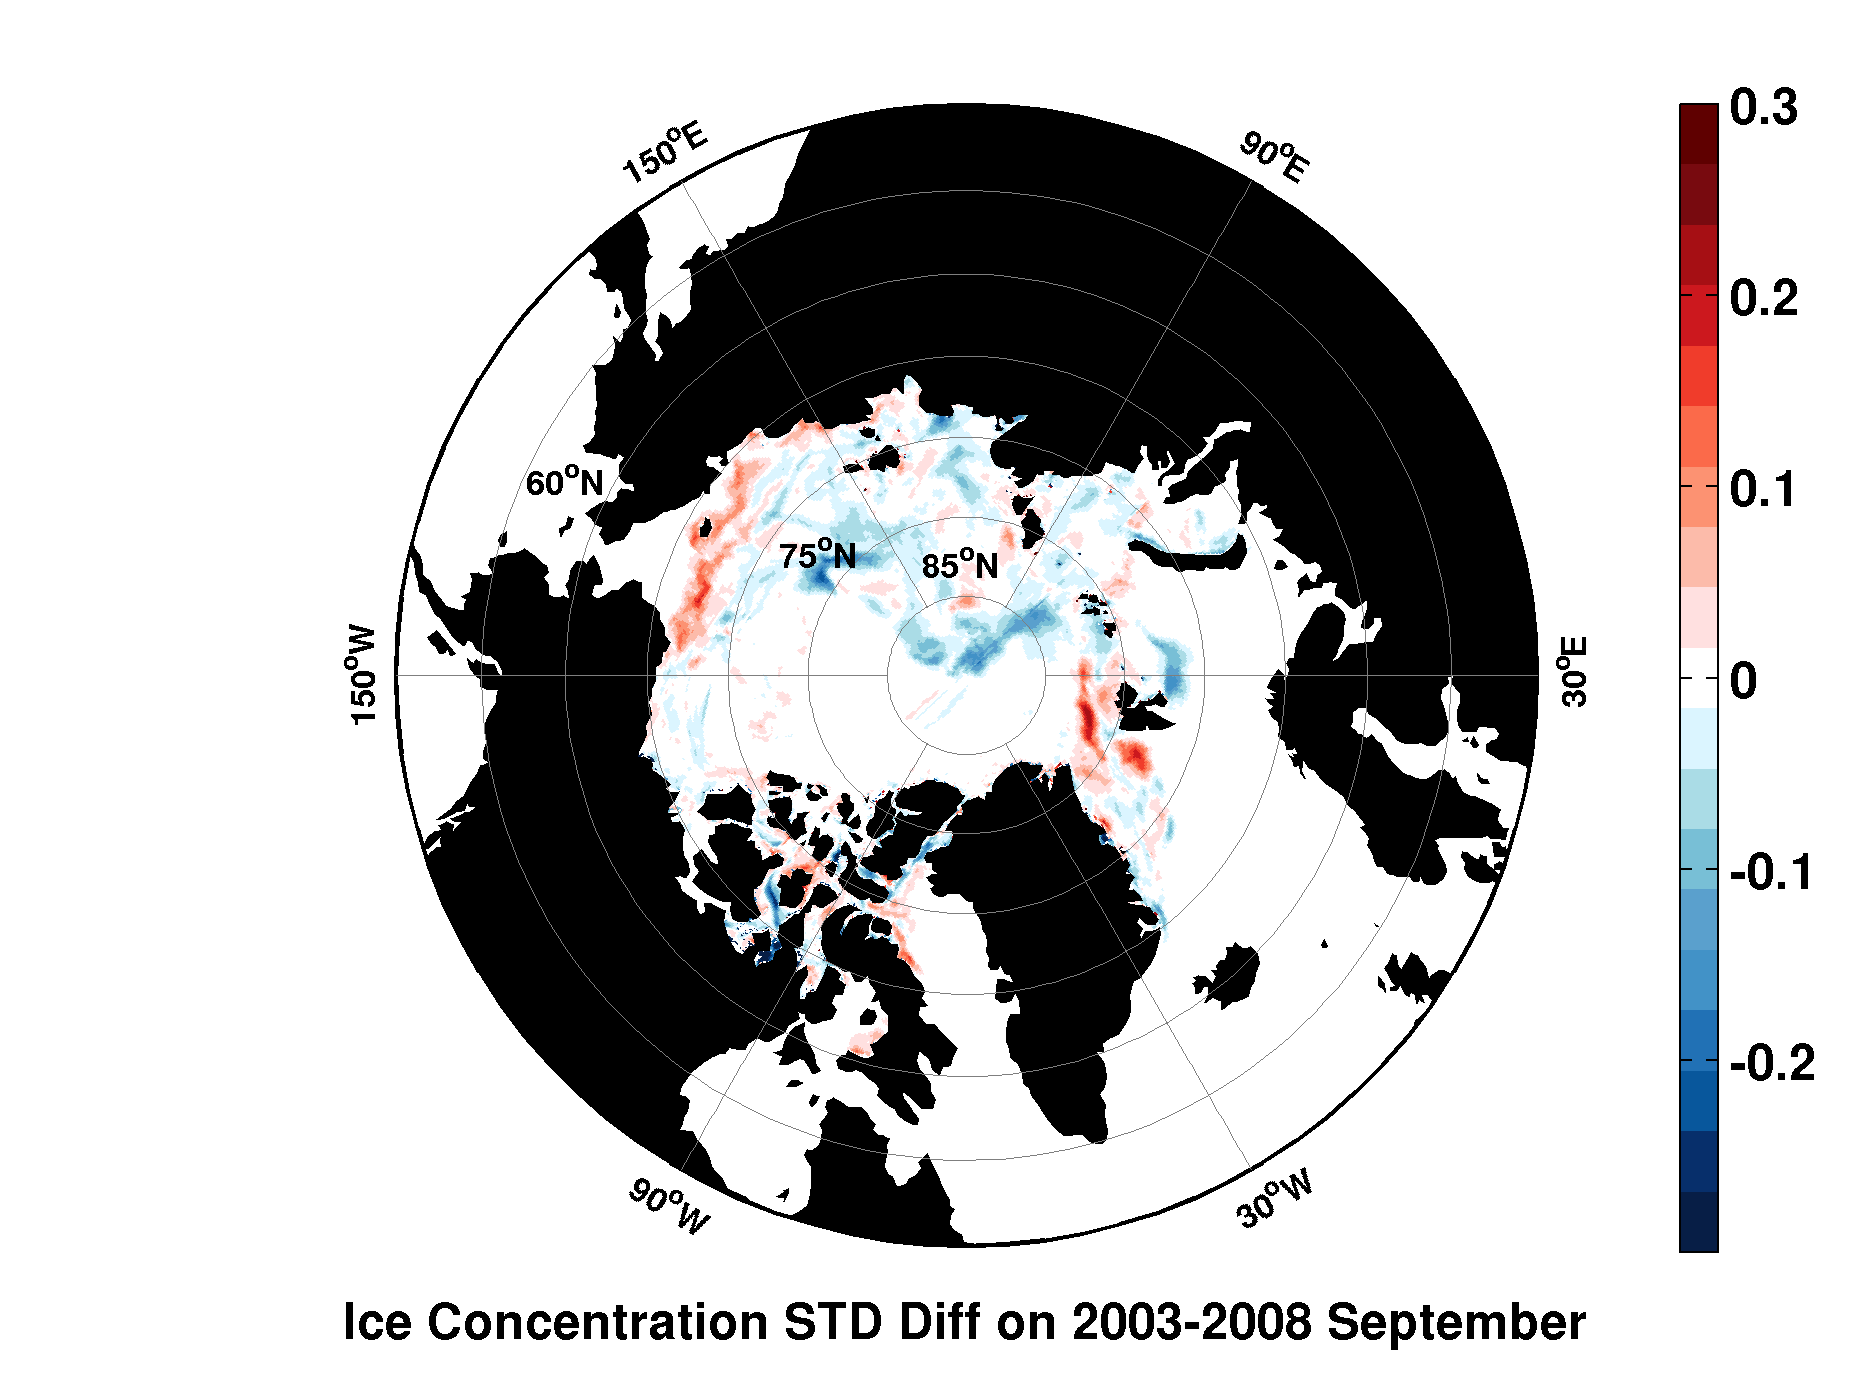
\includegraphics[width=0.9\linewidth]{/home/jingfan/Desktop/Step1/2/Ice_Concentration_STD_Diff_2003-2008_September.png}

\end{frame}

%%%%%%%%%%%%%%%%%%%%%%%%%%%%%%%%%%%%%%%%%%%%%%%%%%%%%%%%%%%%%
\begin{frame}
\frametitle{Sea-Ice Concentration September 2007}
Simply plot Sea-Ice Concentration on each day in September 2007 along with difference plots of different configuration.
\end{frame}

\begin{frame}
\frametitle{Sea-Ice Concentration September 2007}

\begin{columns}
\begin{column}[t]{0.5\linewidth}
\centering
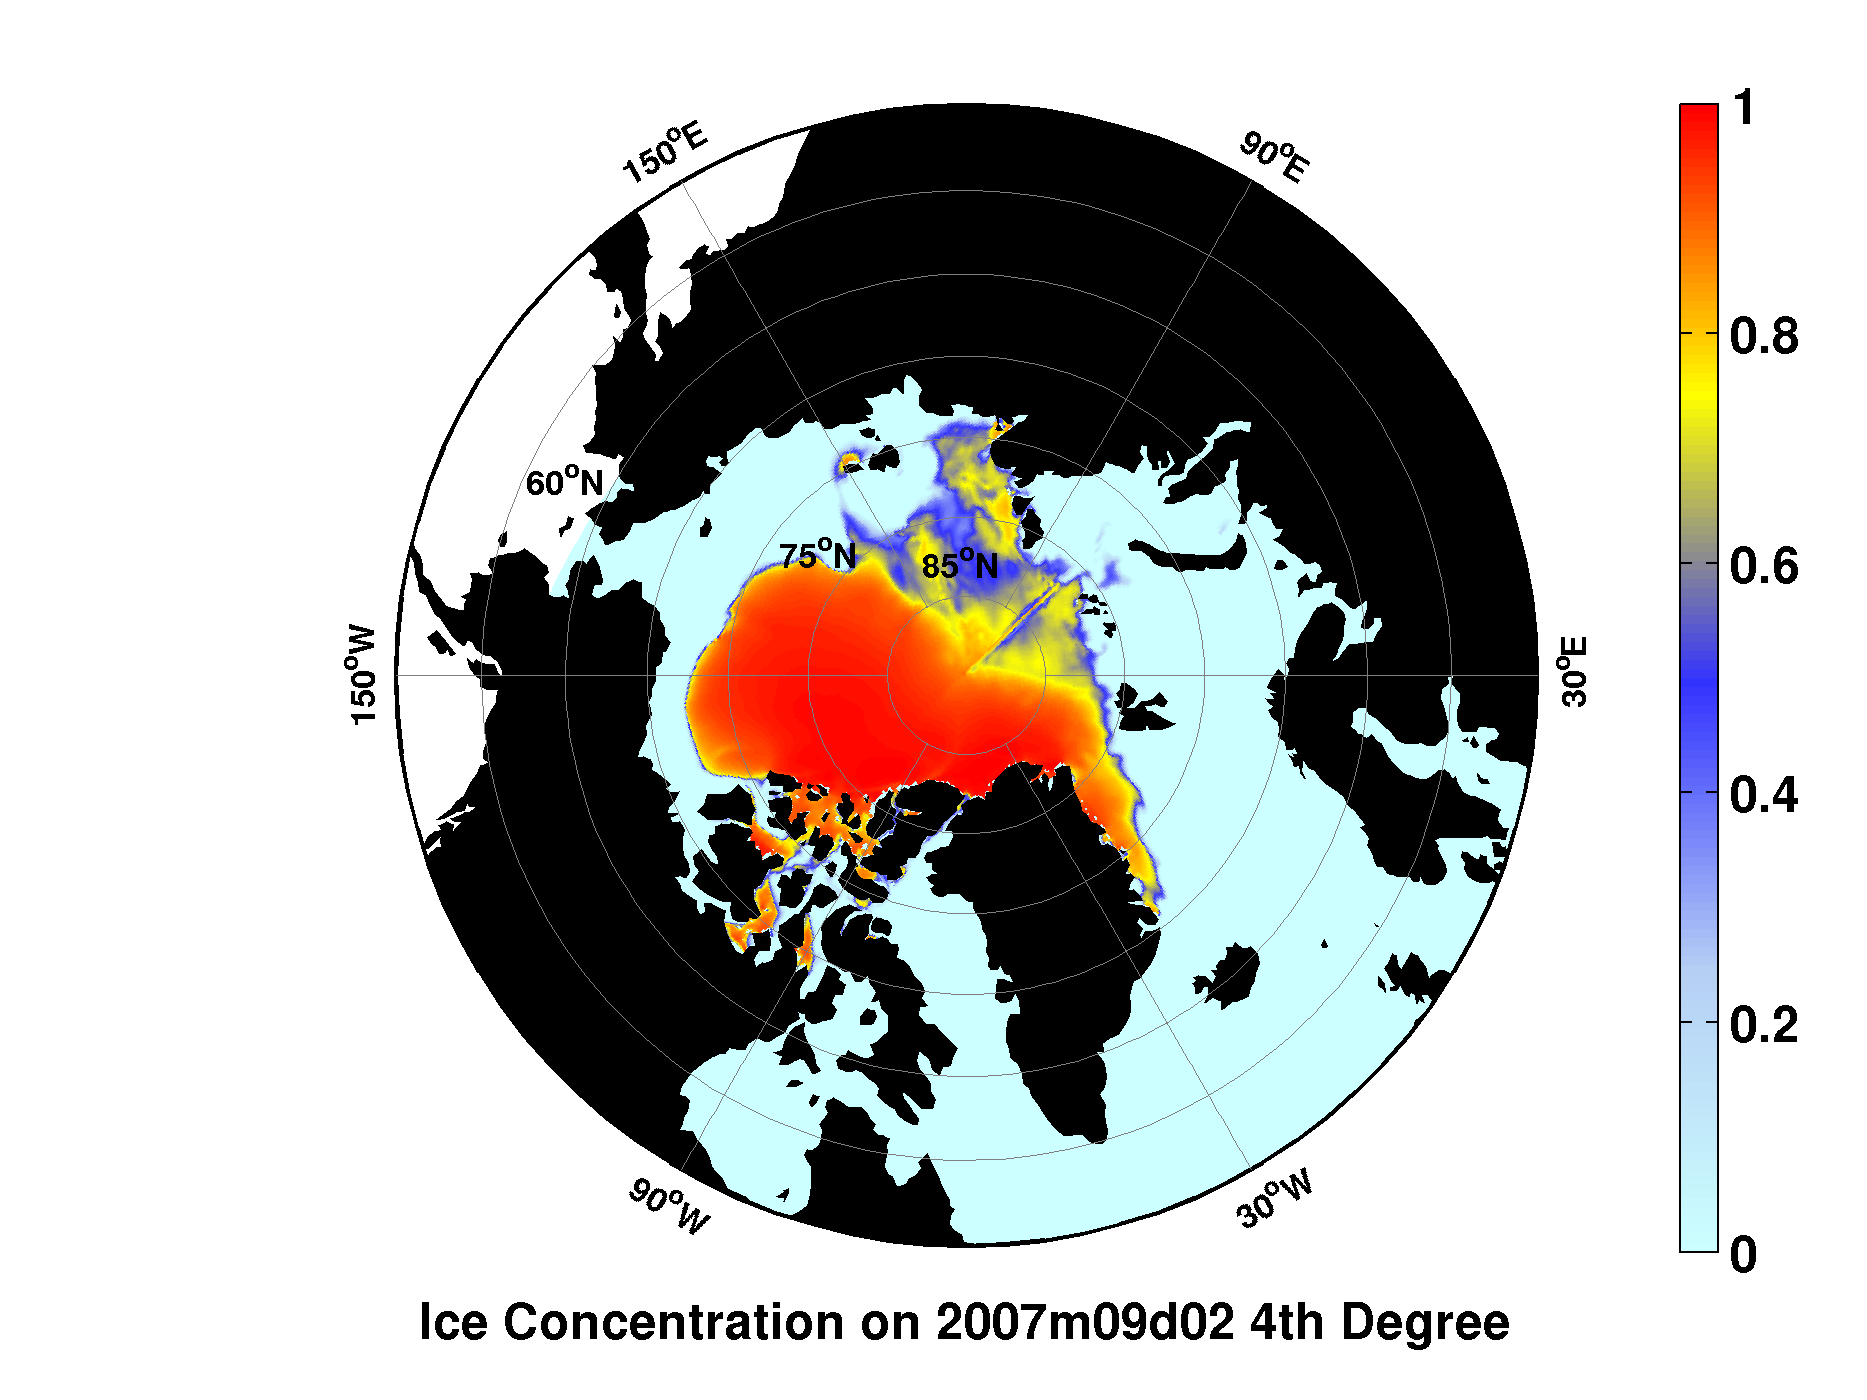
\includegraphics[width=\linewidth]{/home/jingfan/Desktop/Step1/3/Ice_Concentration_2007m09d02_4th_Degree.png}
\end{column}
\begin{column}[t]{0.5\linewidth}
\centering
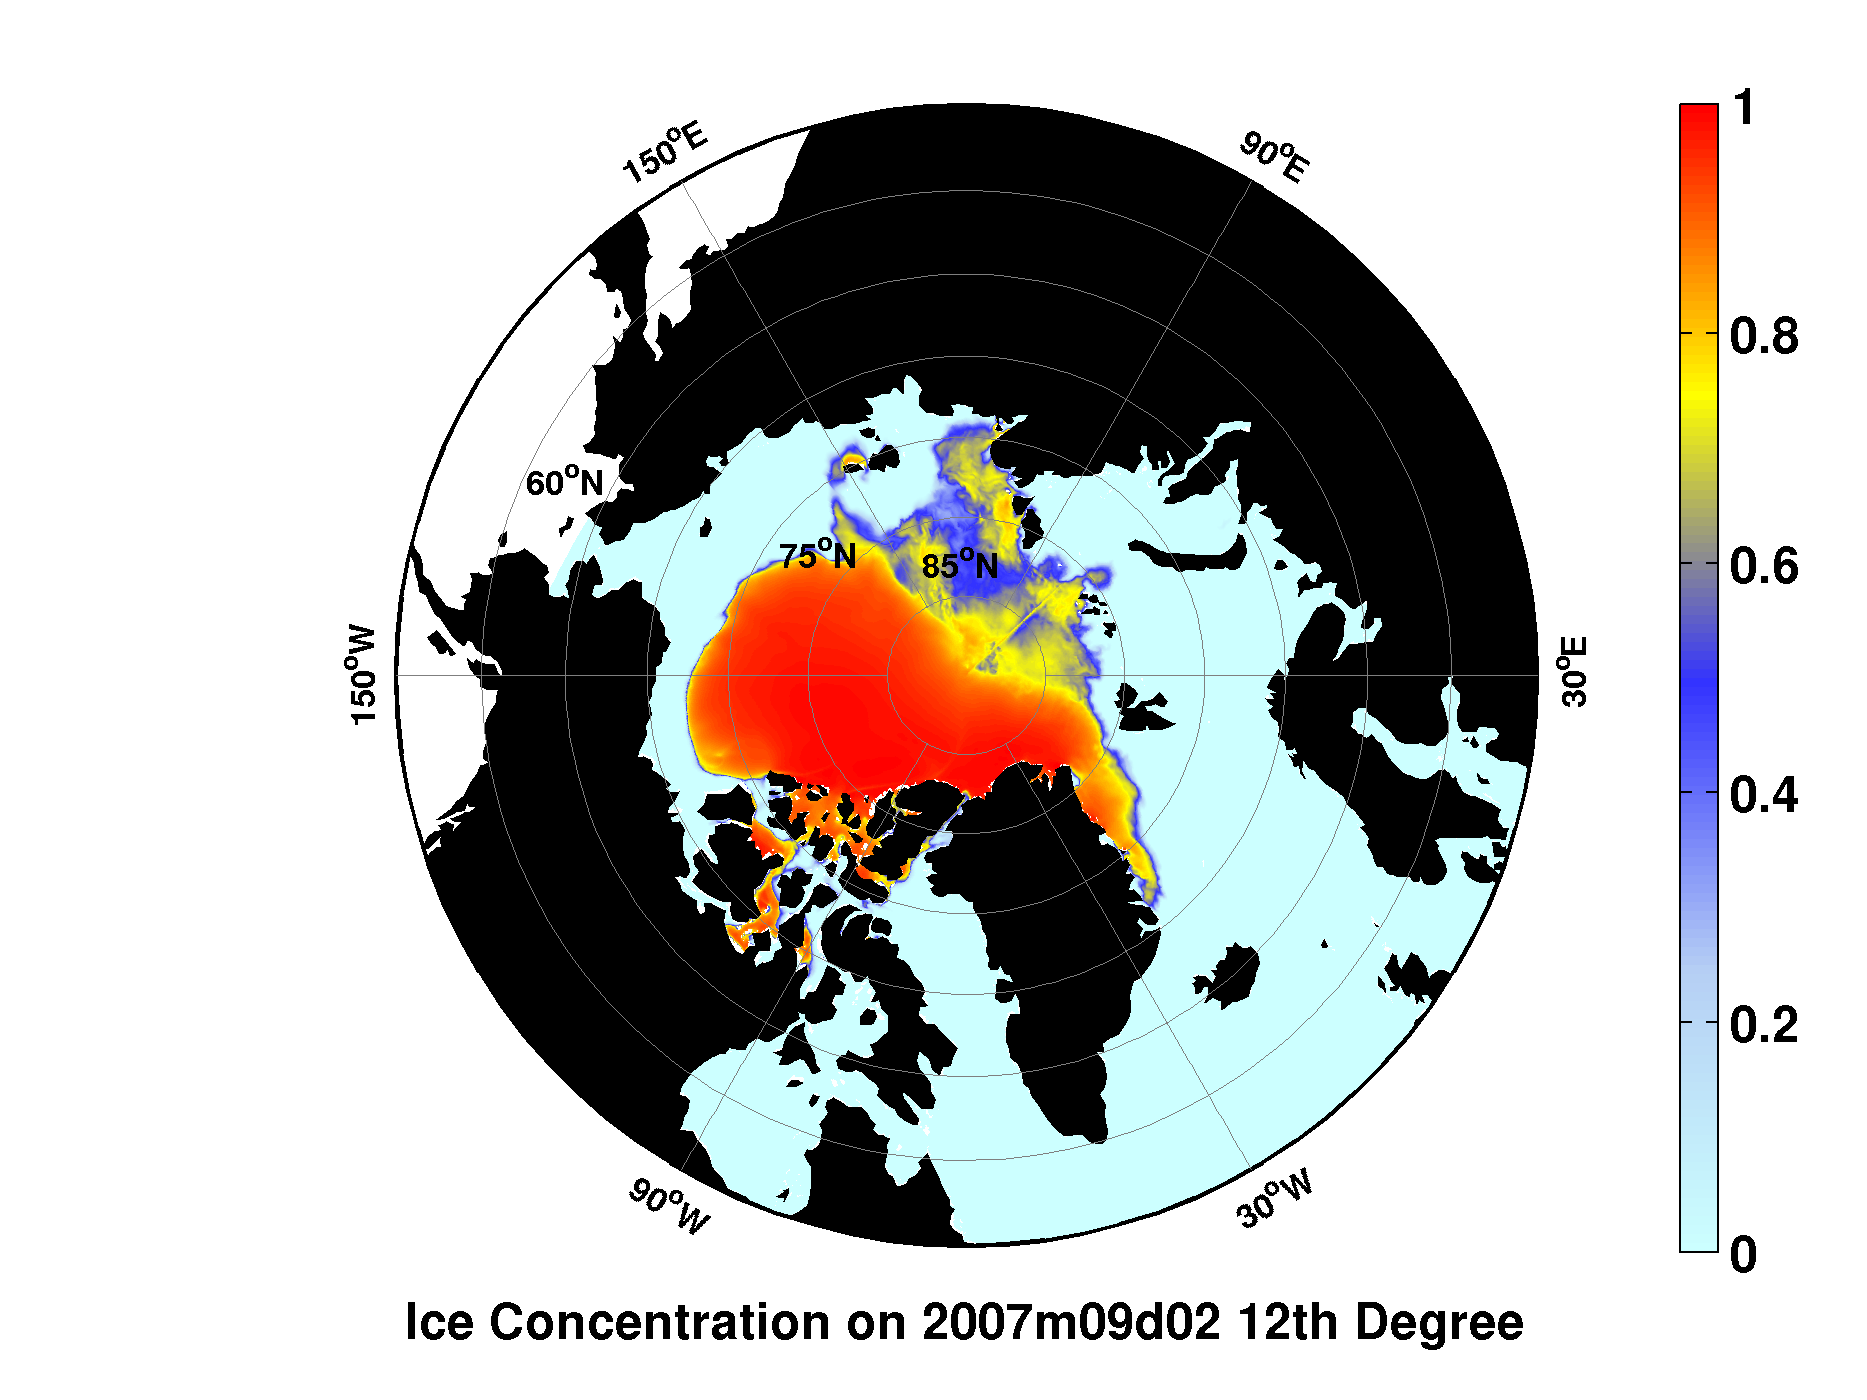
\includegraphics[width=\linewidth]{/home/jingfan/Desktop/Step1/3/Ice_Concentration_2007m09d02_12th_Degree.png}
\end{column}
\end{columns}

\end{frame}

\begin{frame}
\frametitle{Sea-Ice Concentration September 2007 Difference(ANHA12-ANHA4)}

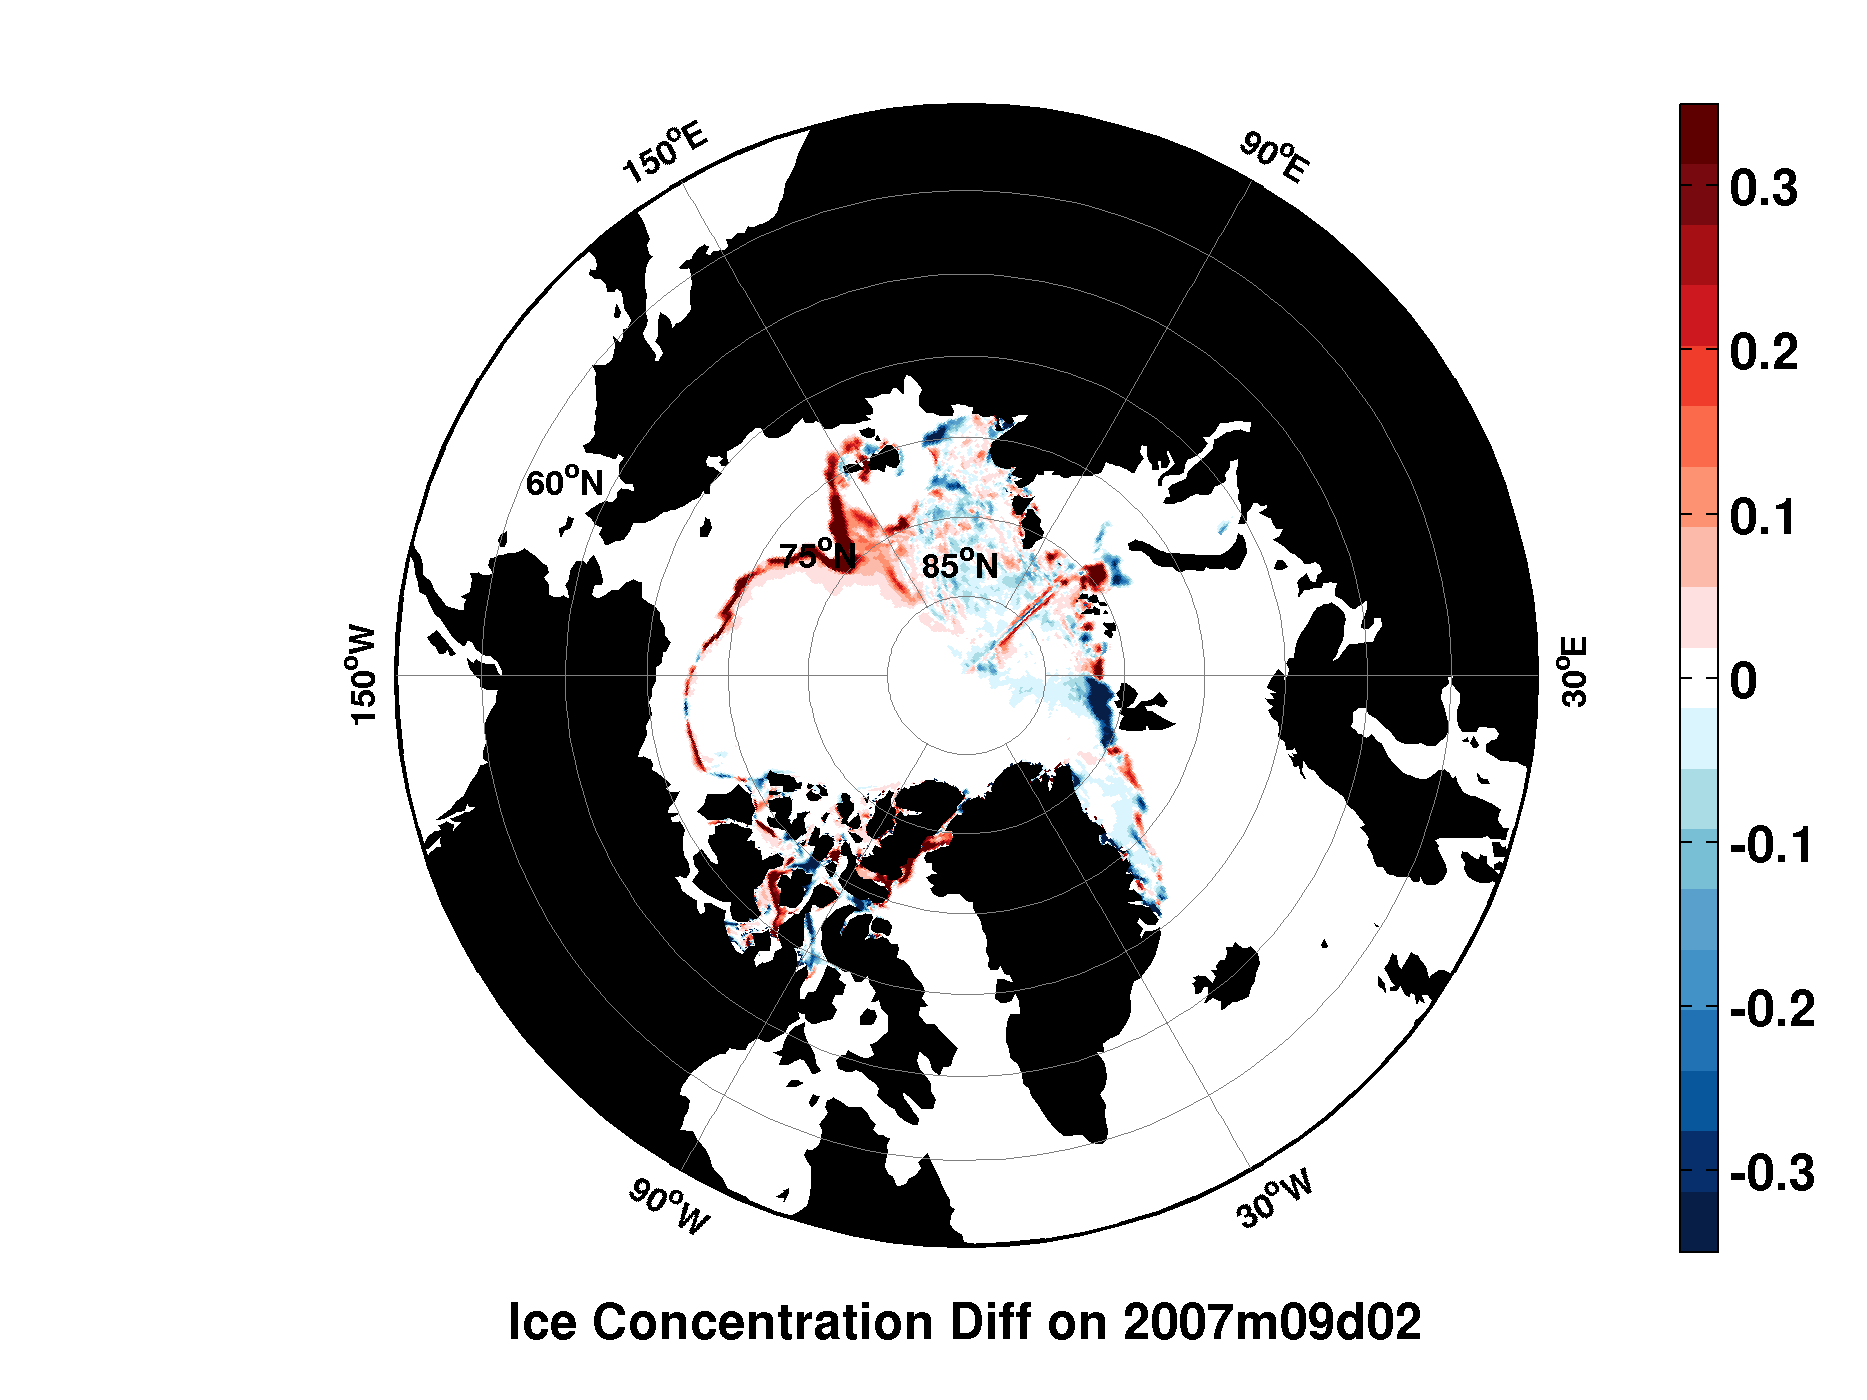
\includegraphics[width=0.9\linewidth]{/home/jingfan/Desktop/Step1/3/Ice_Concentration_Diff_2007m09d02.png}

\end{frame}

\begin{frame}
\frametitle{Sea-Ice Concentration September 2007}

\begin{columns}
\begin{column}[t]{0.5\linewidth}
\centering
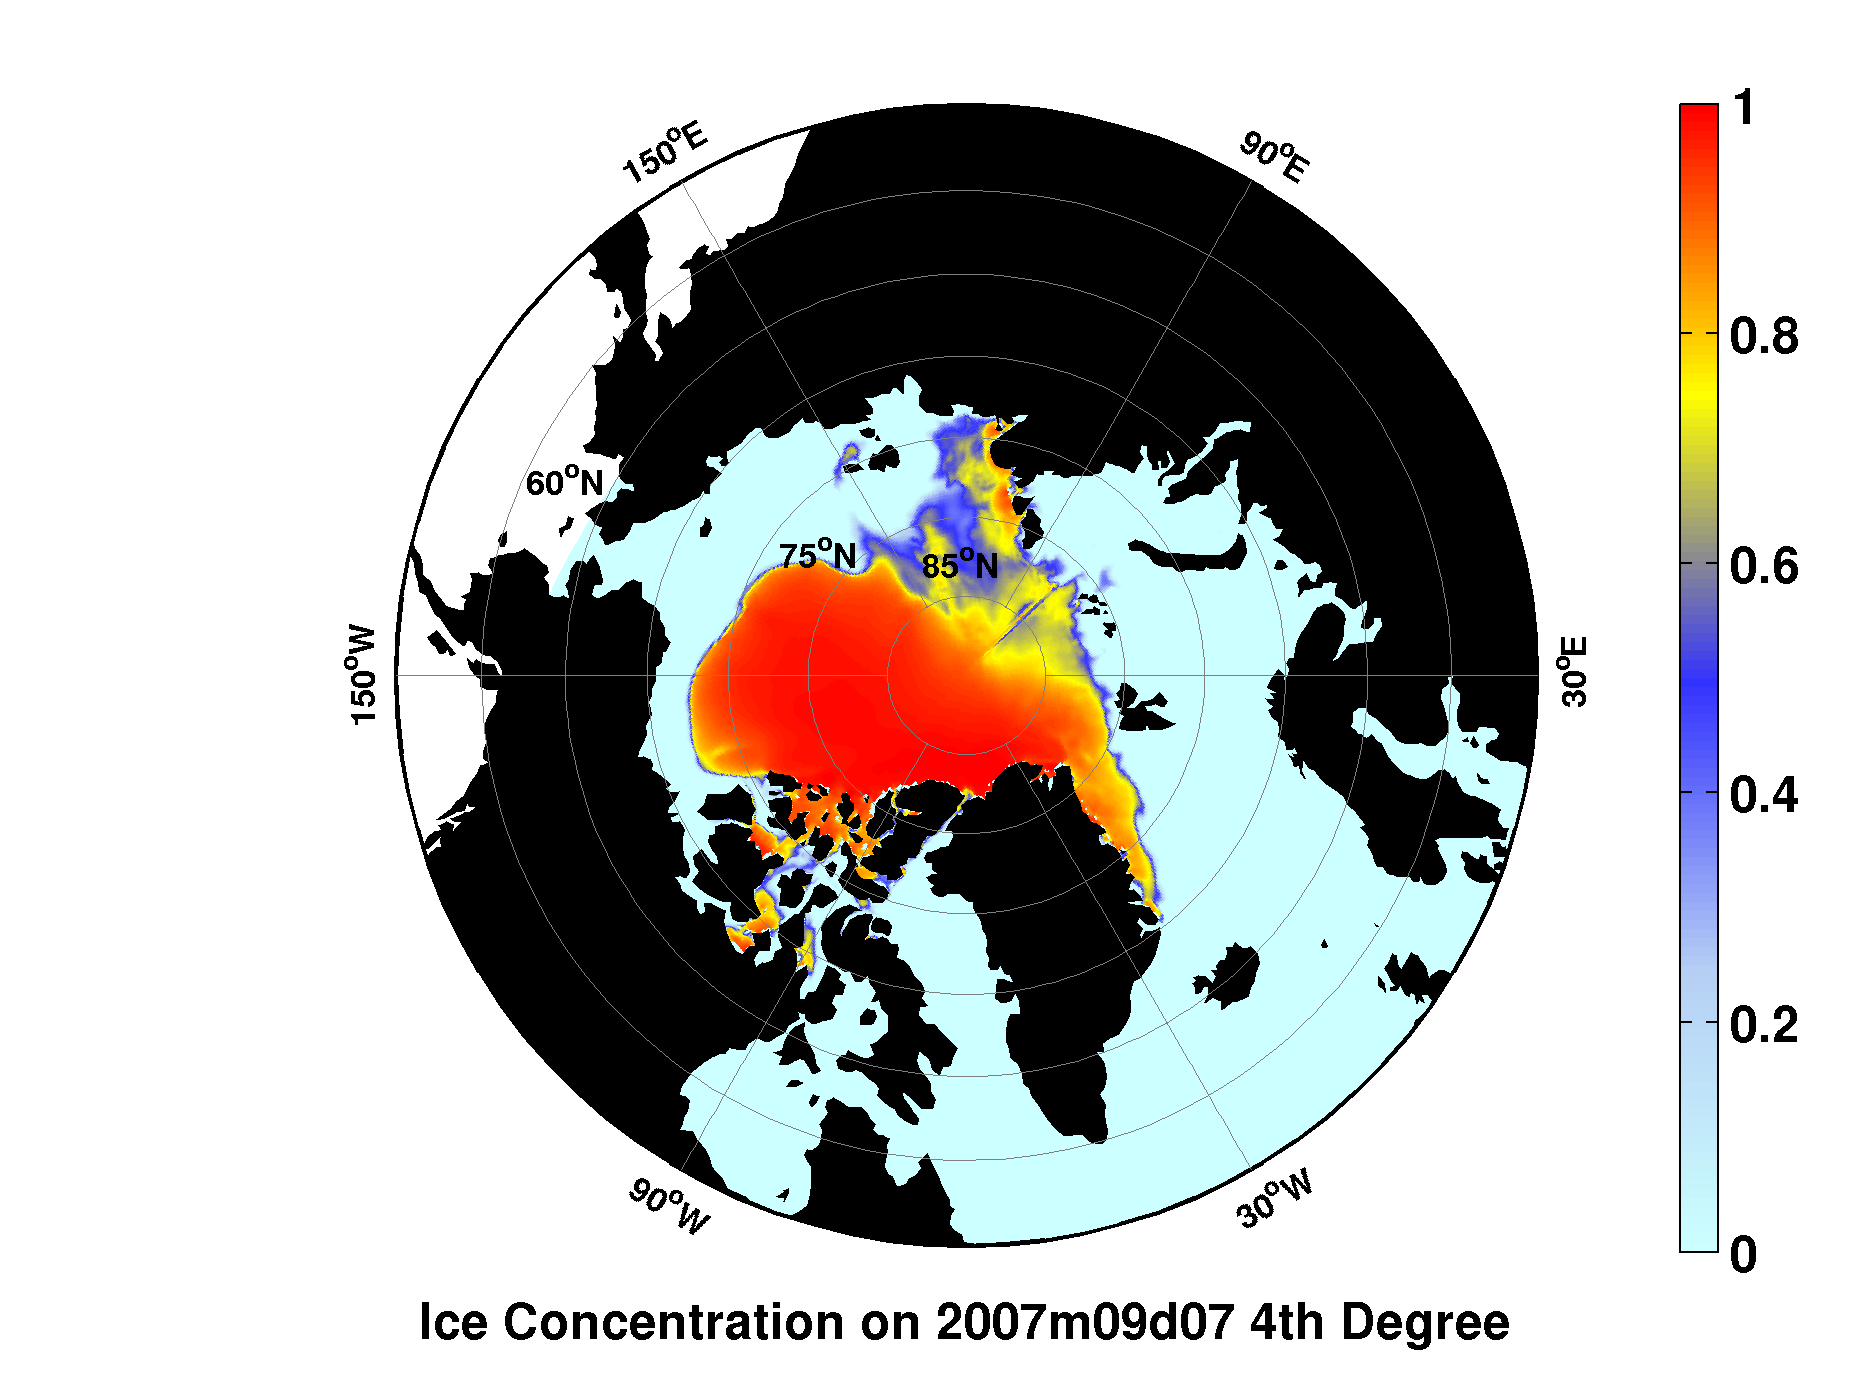
\includegraphics[width=\linewidth]{/home/jingfan/Desktop/Step1/3/Ice_Concentration_2007m09d07_4th_Degree.png}
\end{column}
\begin{column}[t]{0.5\linewidth}
\centering
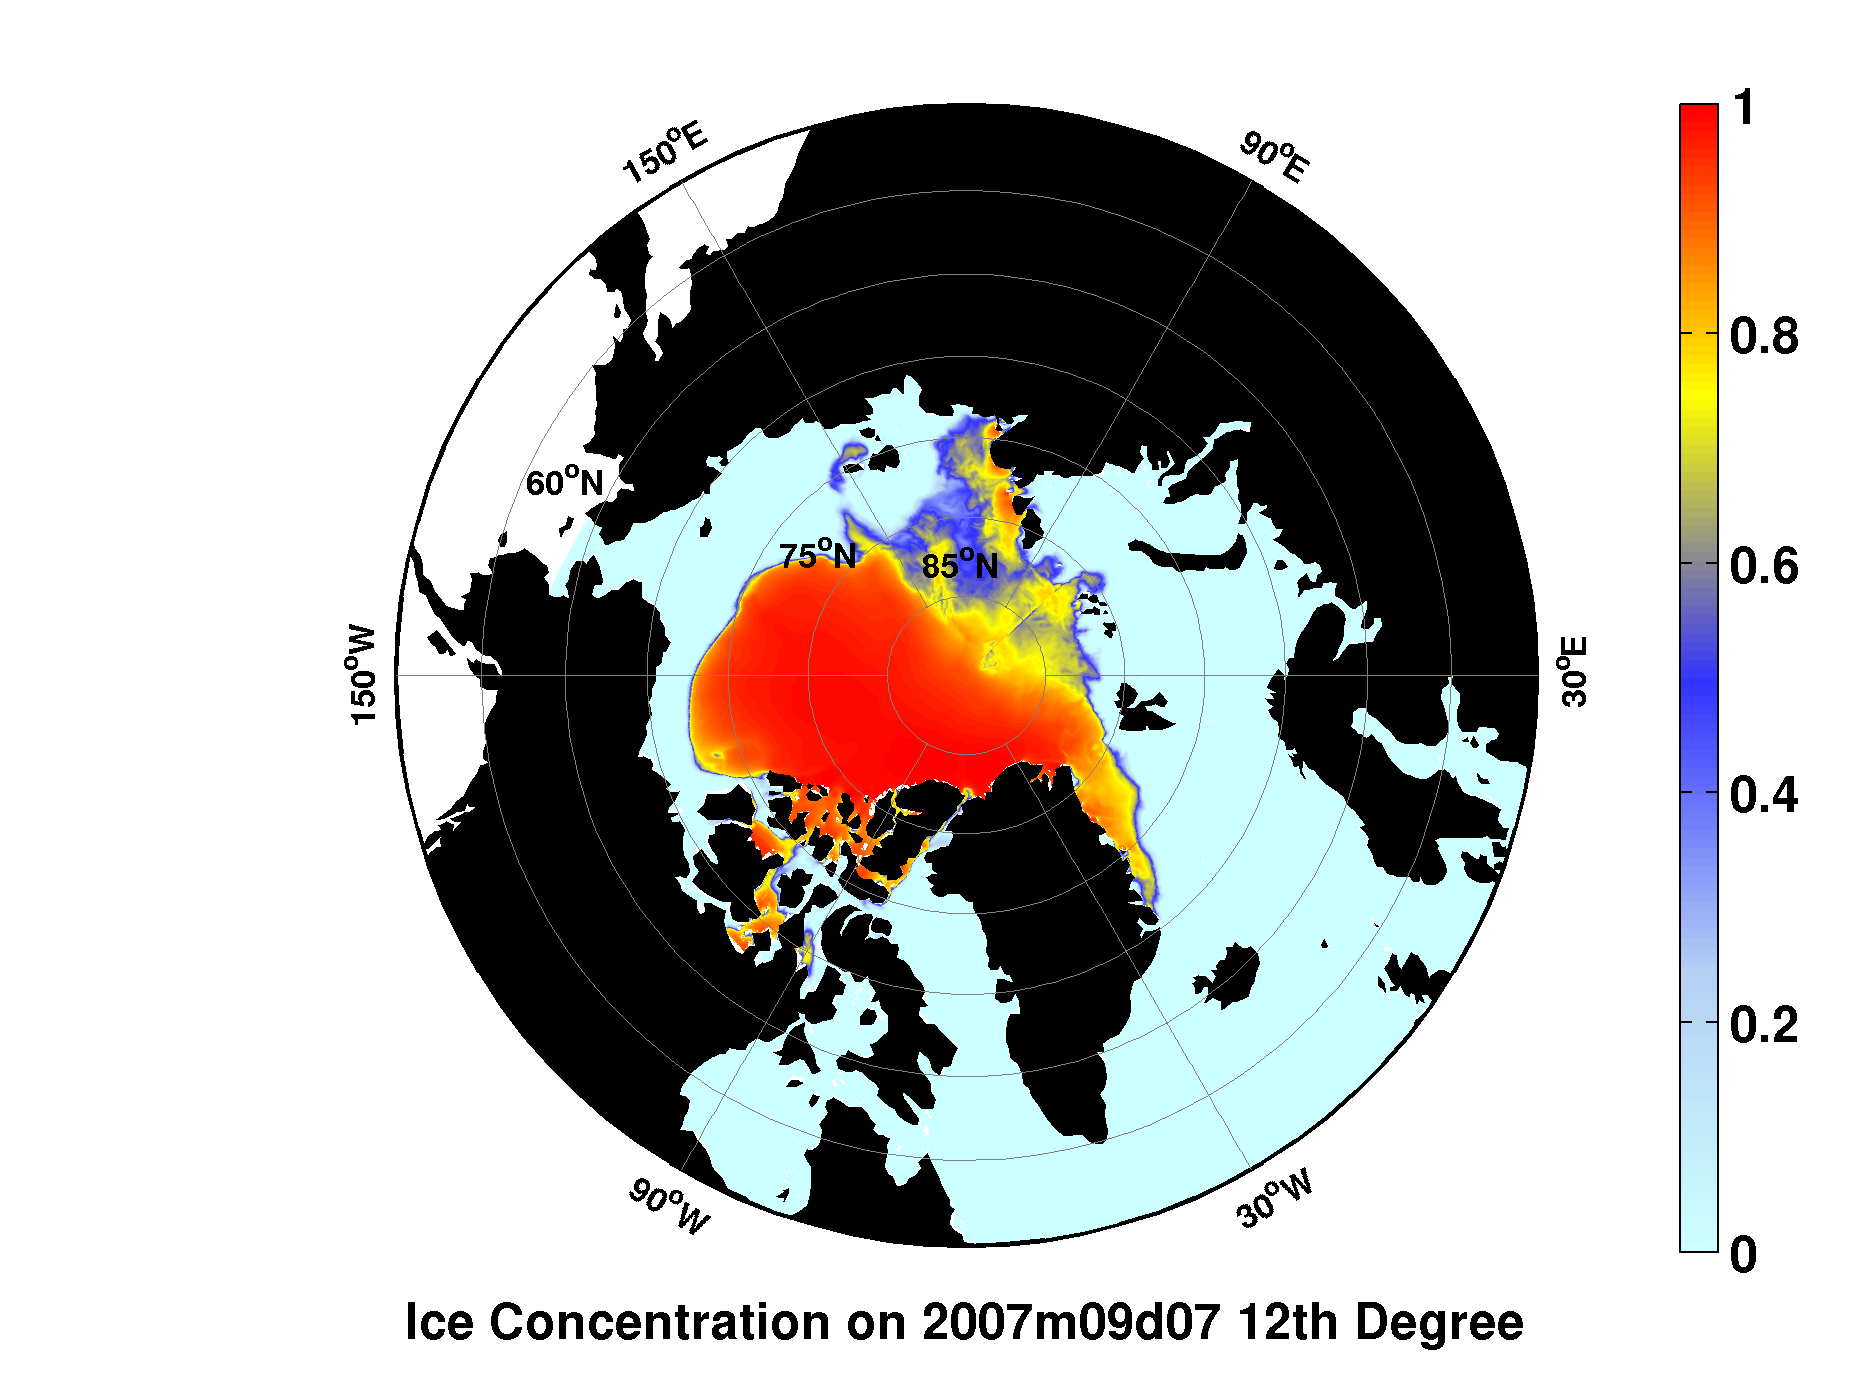
\includegraphics[width=\linewidth]{/home/jingfan/Desktop/Step1/3/Ice_Concentration_2007m09d07_12th_Degree.png}
\end{column}
\end{columns}

\end{frame}

\begin{frame}
\frametitle{Sea-Ice Concentration September 2007 Difference(ANHA12-ANHA4)}

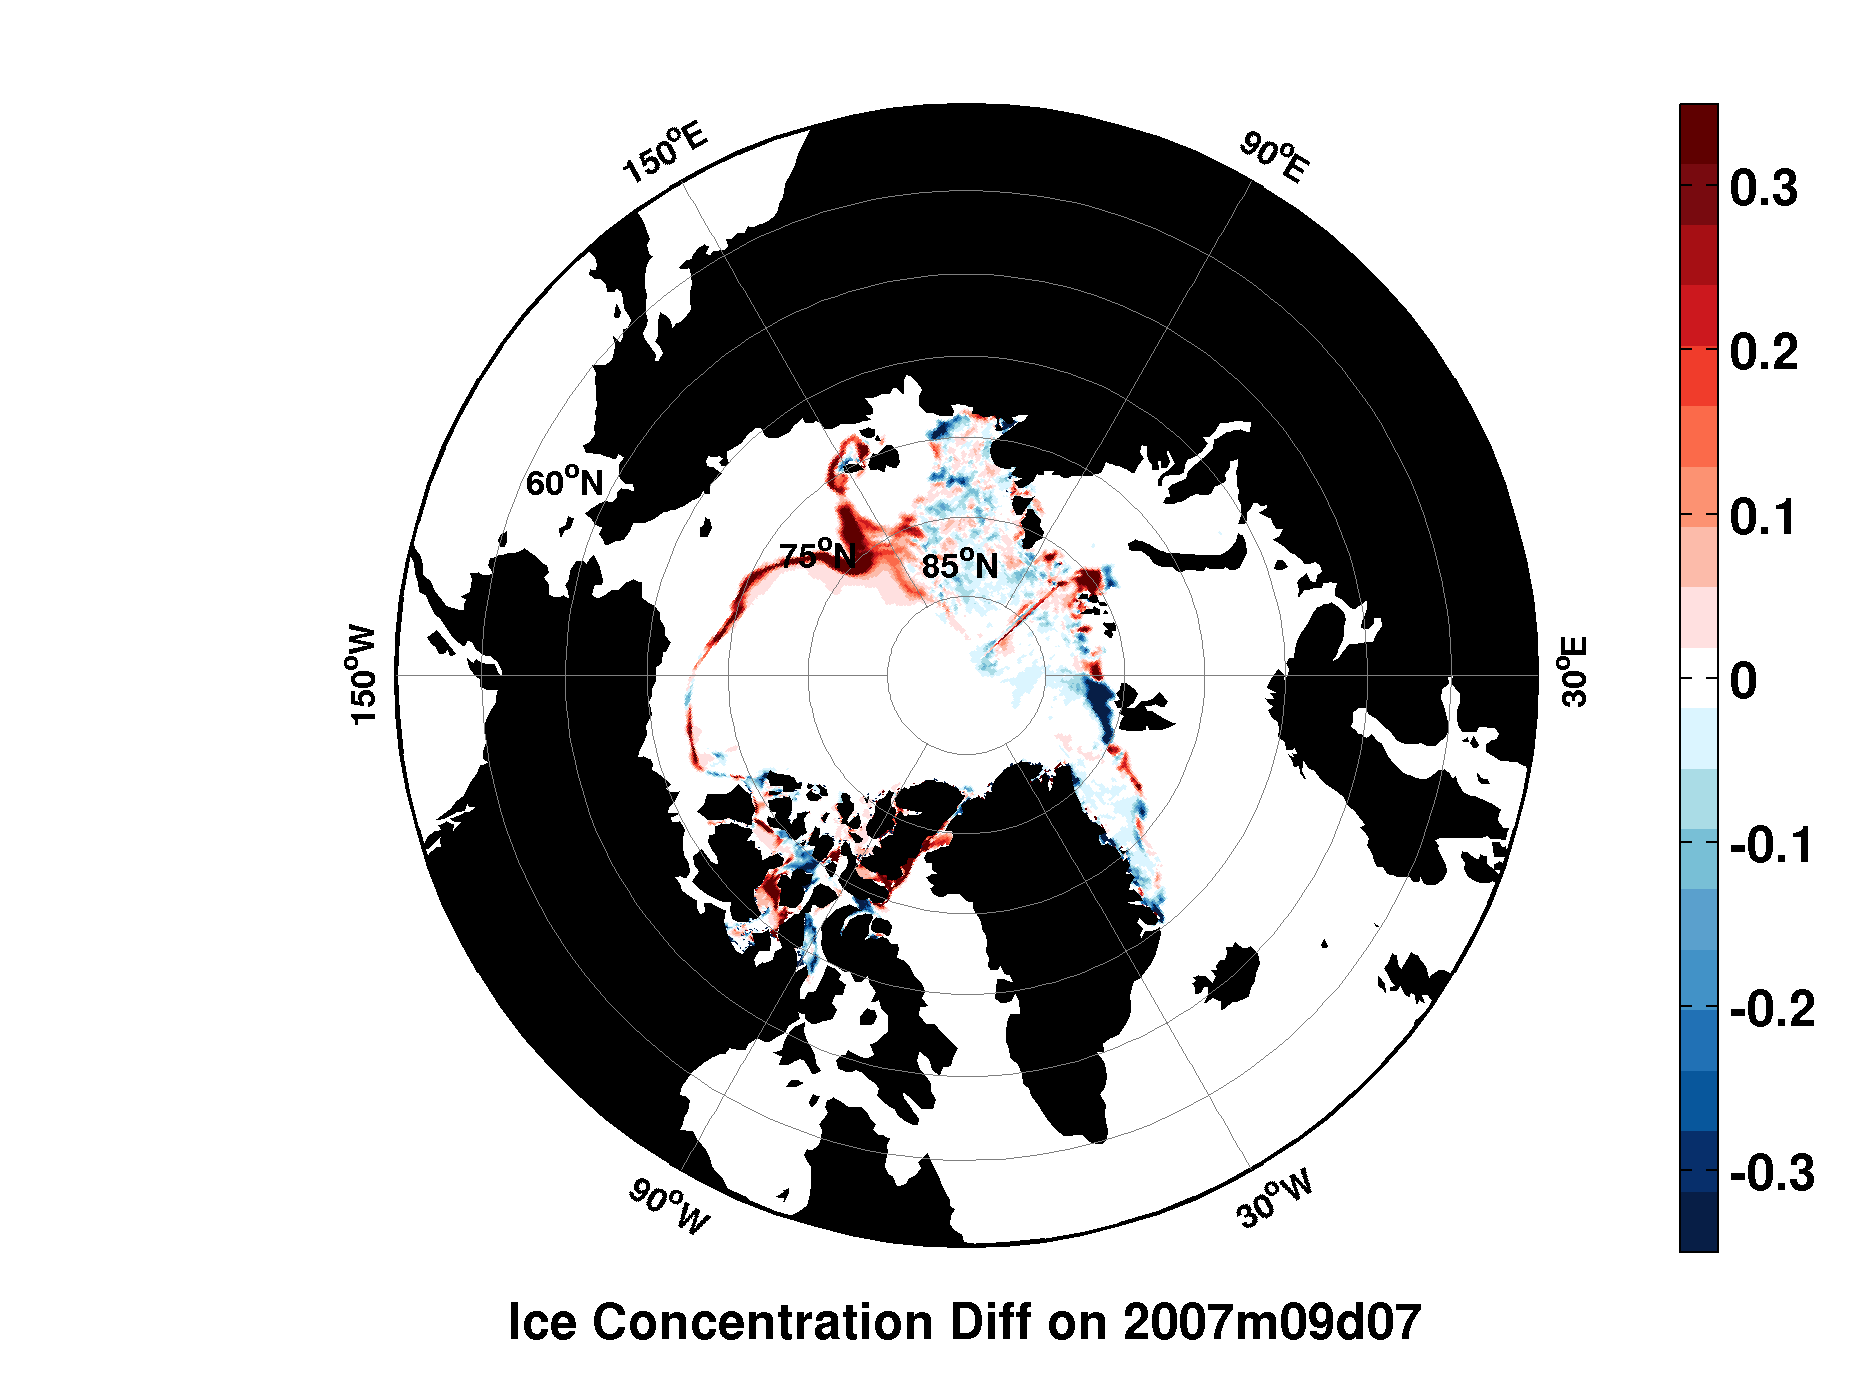
\includegraphics[width=0.9\linewidth]{/home/jingfan/Desktop/Step1/3/Ice_Concentration_Diff_2007m09d07.png}

\end{frame}

\begin{frame}
\frametitle{Sea-Ice Concentration September 2007}

\begin{columns}
\begin{column}[t]{0.5\linewidth}
\centering
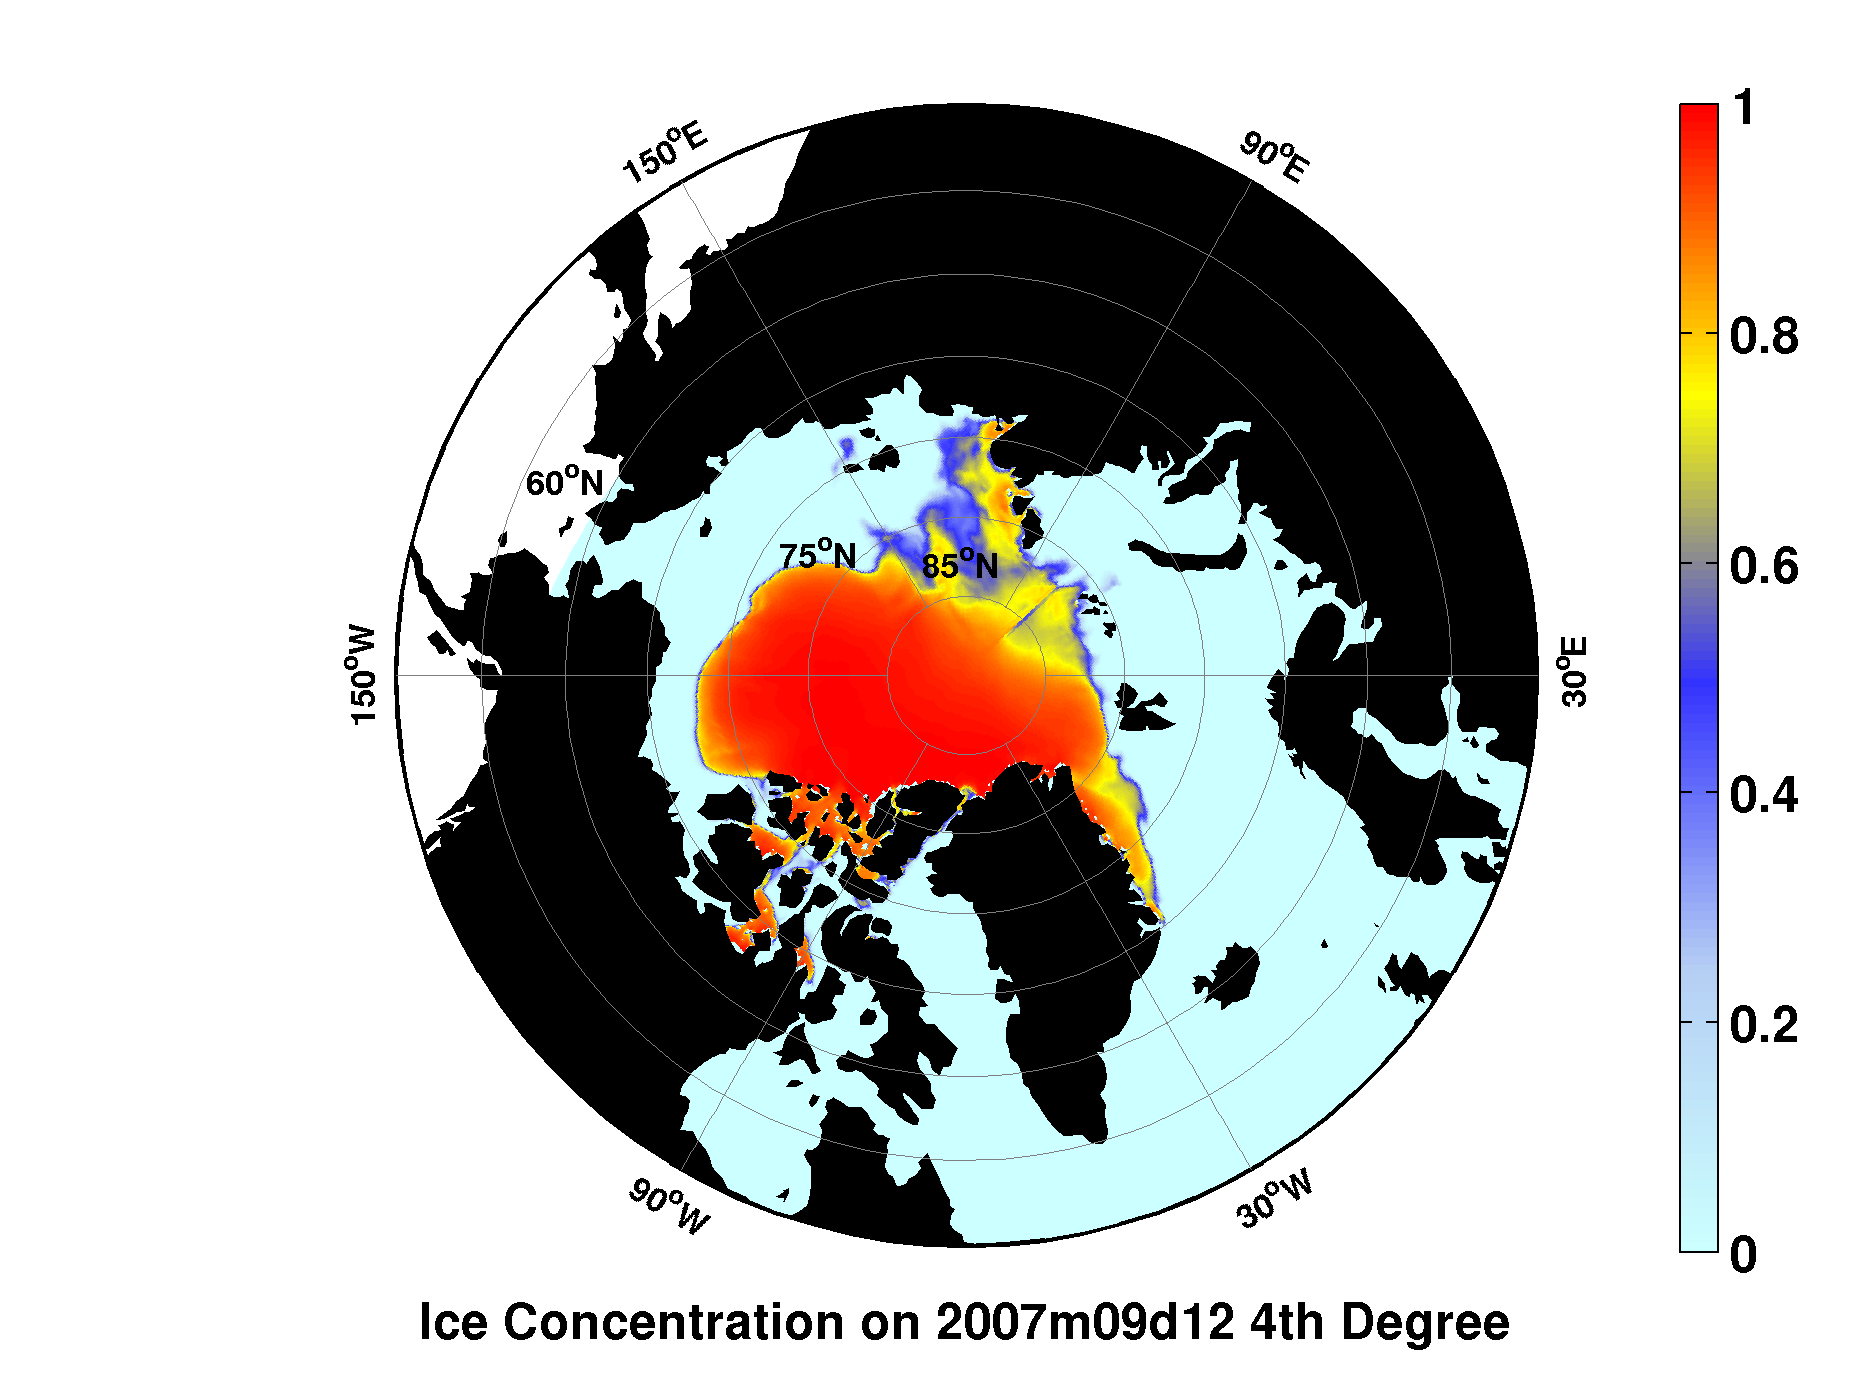
\includegraphics[width=\linewidth]{/home/jingfan/Desktop/Step1/3/Ice_Concentration_2007m09d12_4th_Degree.png}
\end{column}
\begin{column}[t]{0.5\linewidth}
\centering
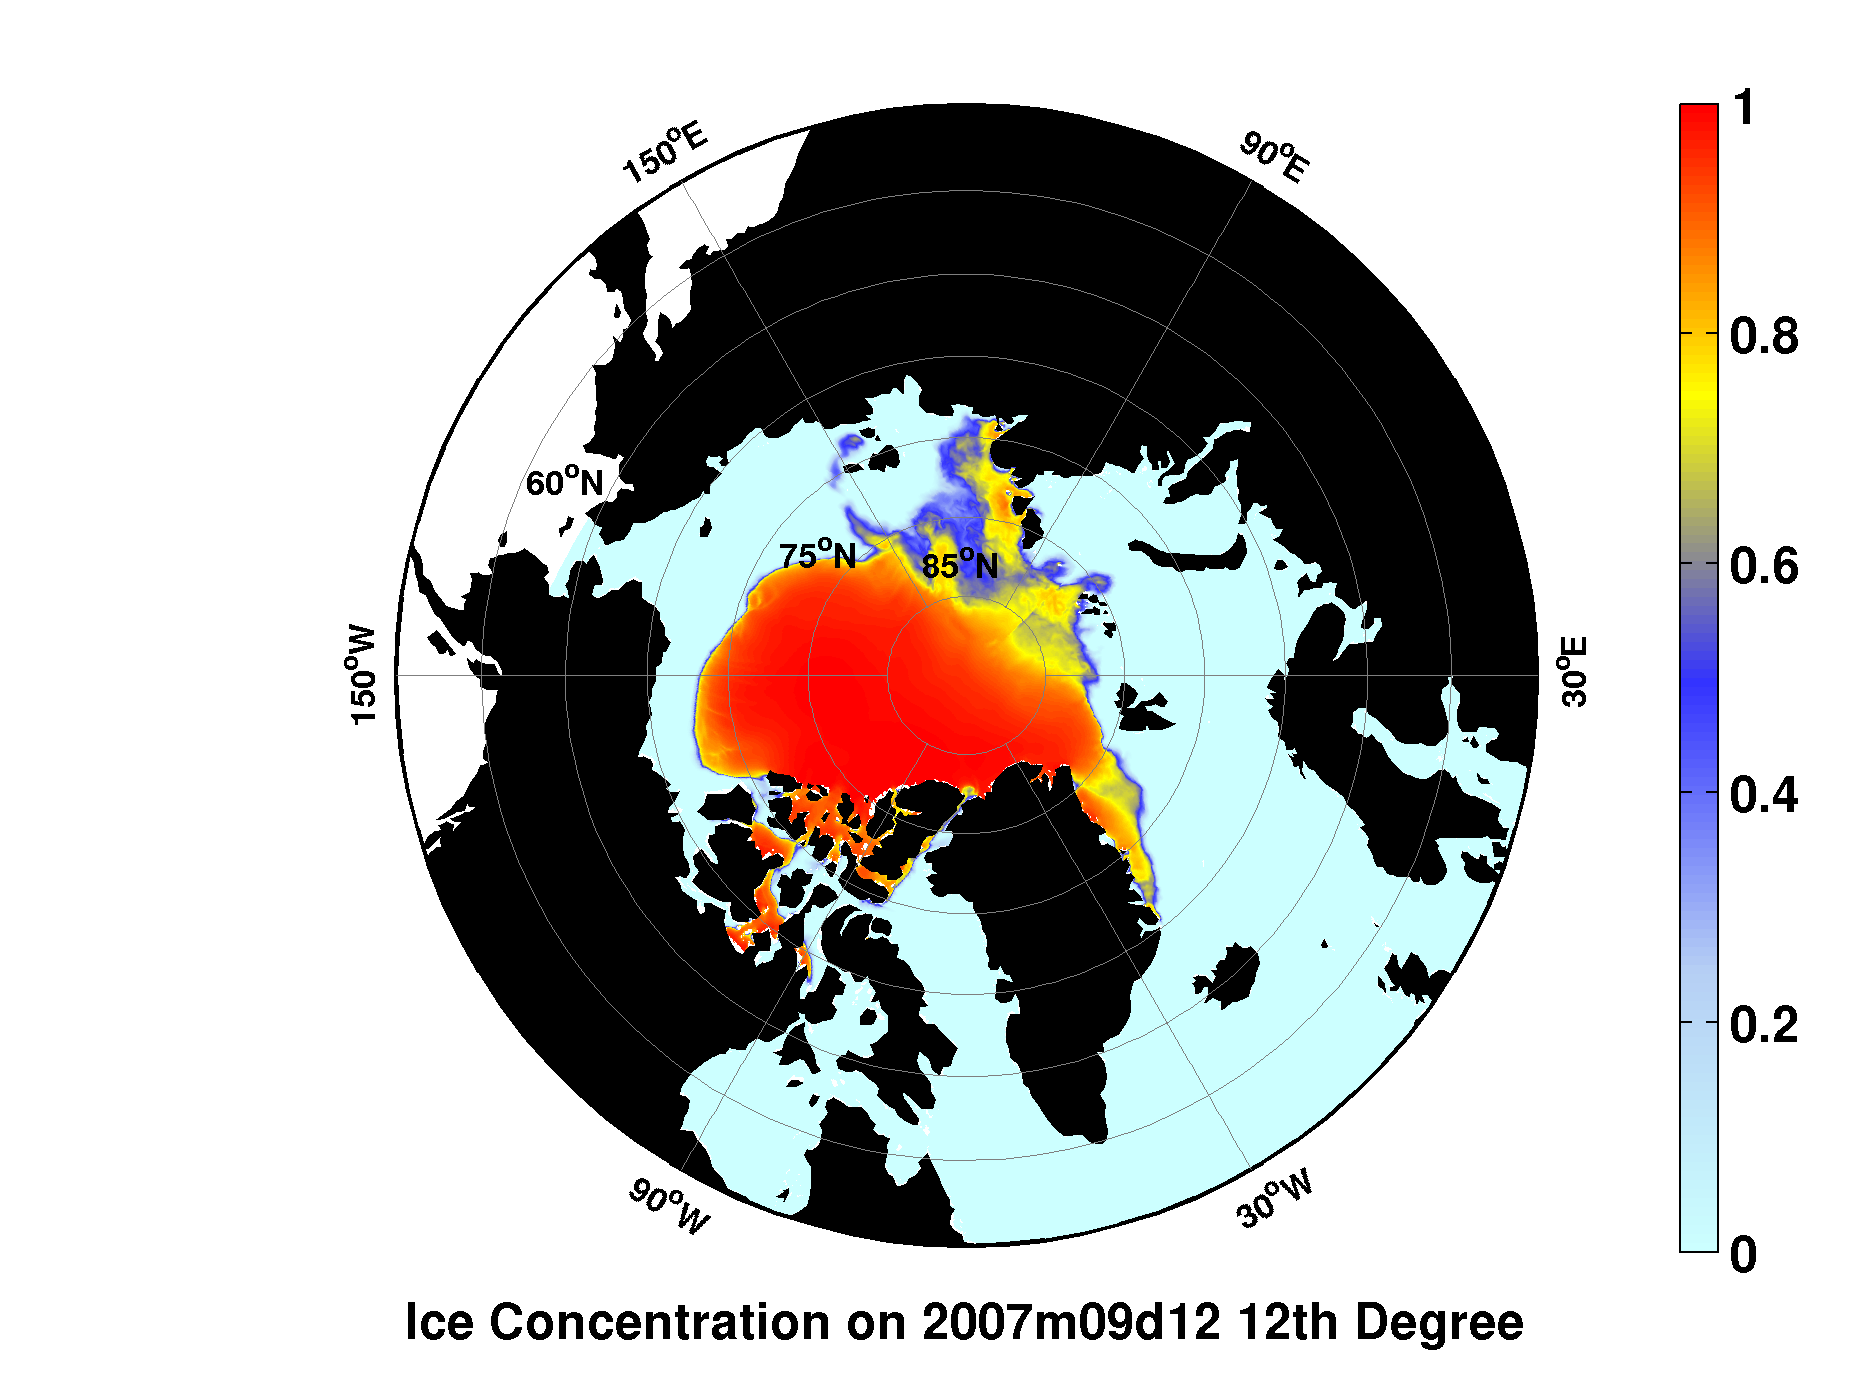
\includegraphics[width=\linewidth]{/home/jingfan/Desktop/Step1/3/Ice_Concentration_2007m09d12_12th_Degree.png}
\end{column}
\end{columns}

\end{frame}

\begin{frame}
\frametitle{Sea-Ice Concentration September 2007 Difference(ANHA12-ANHA4)}

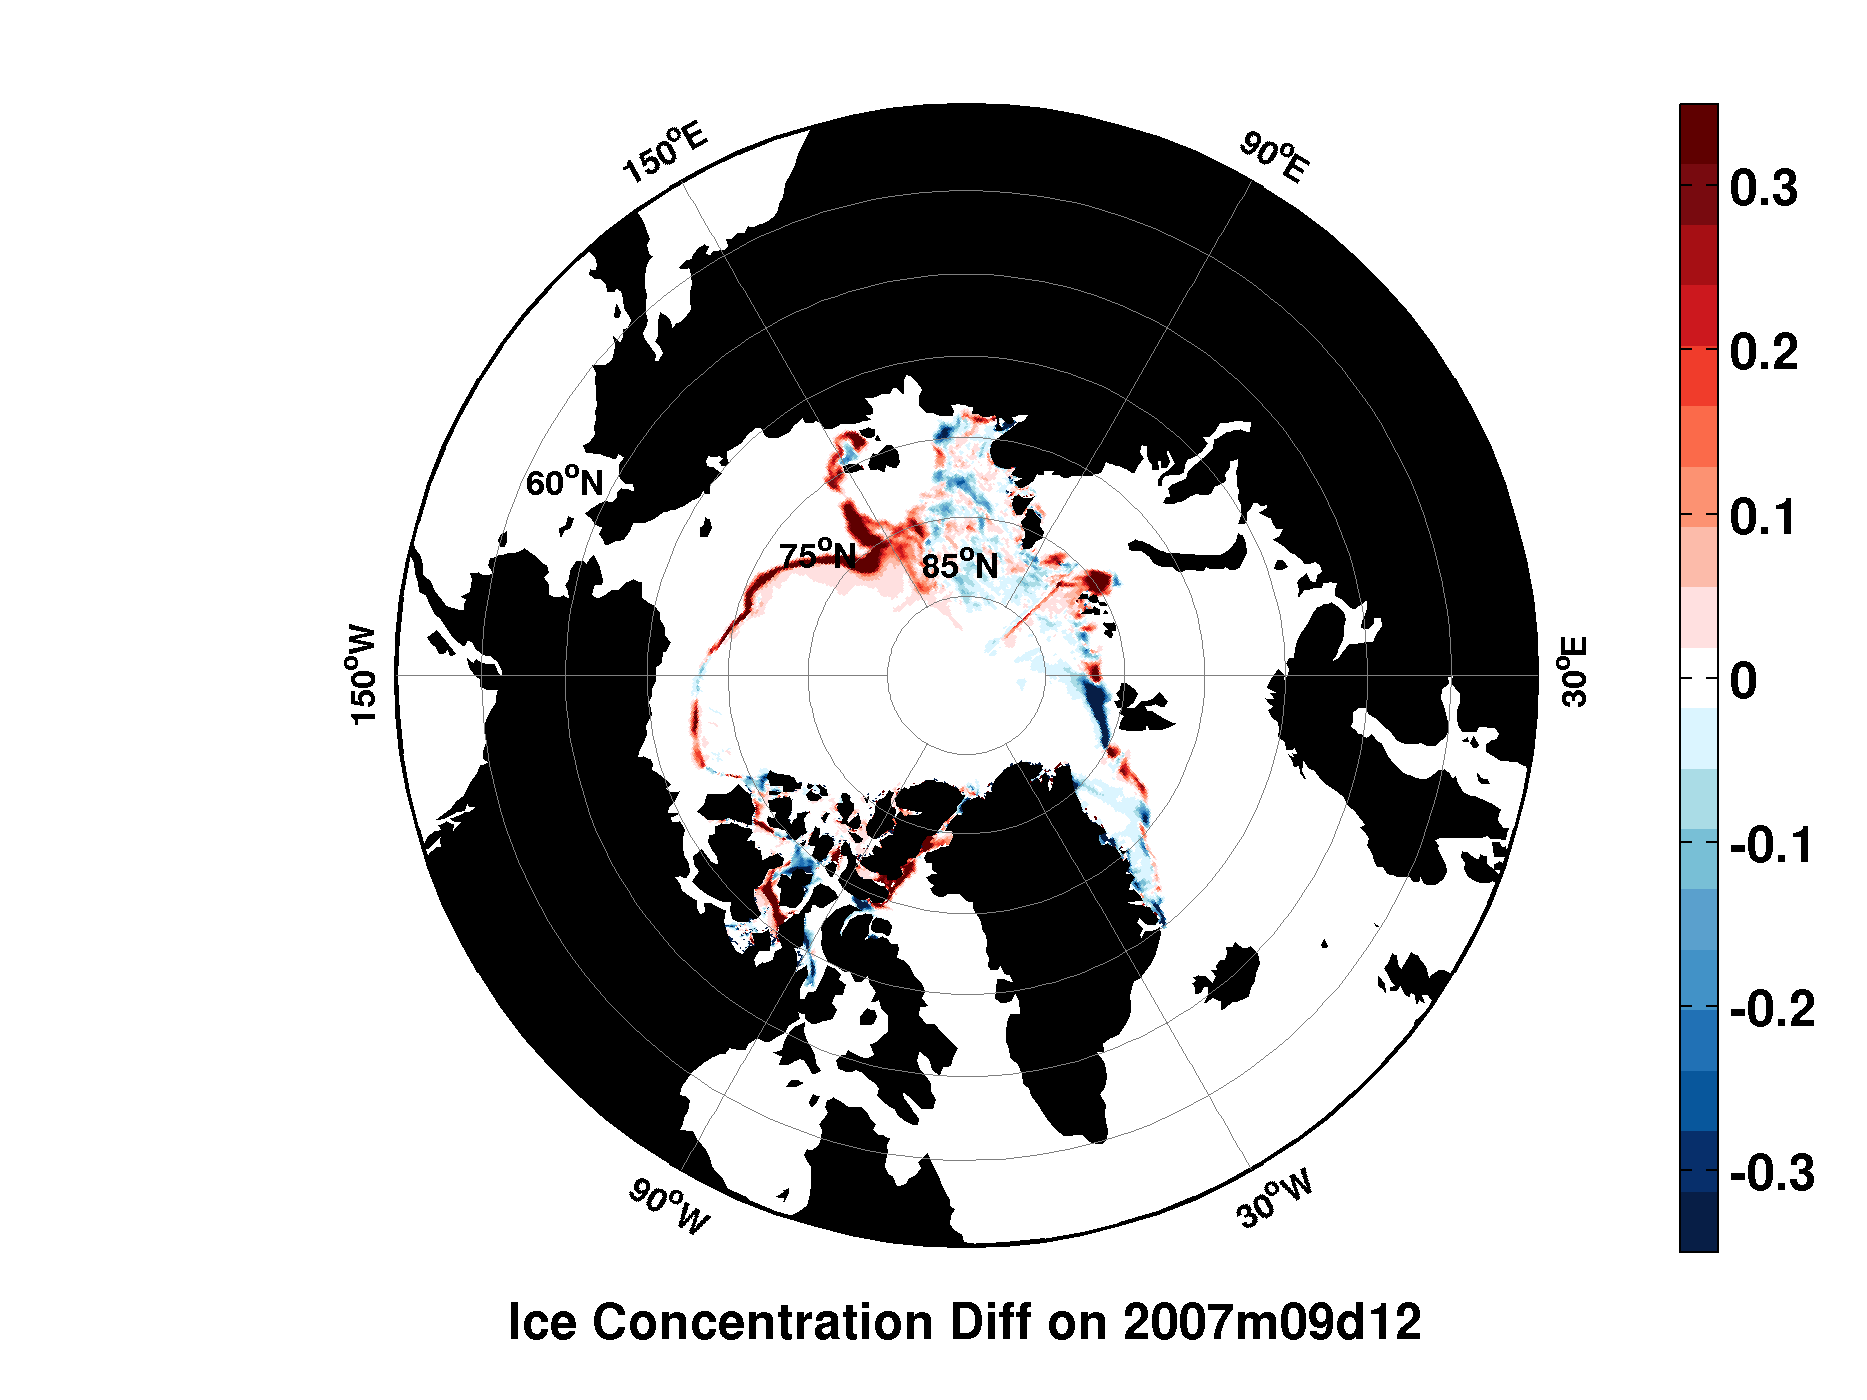
\includegraphics[width=0.9\linewidth]{/home/jingfan/Desktop/Step1/3/Ice_Concentration_Diff_2007m09d12.png}

\end{frame}

\begin{frame}
\frametitle{Sea-Ice Concentration September 2007}

\begin{columns}
\begin{column}[t]{0.5\linewidth}
\centering
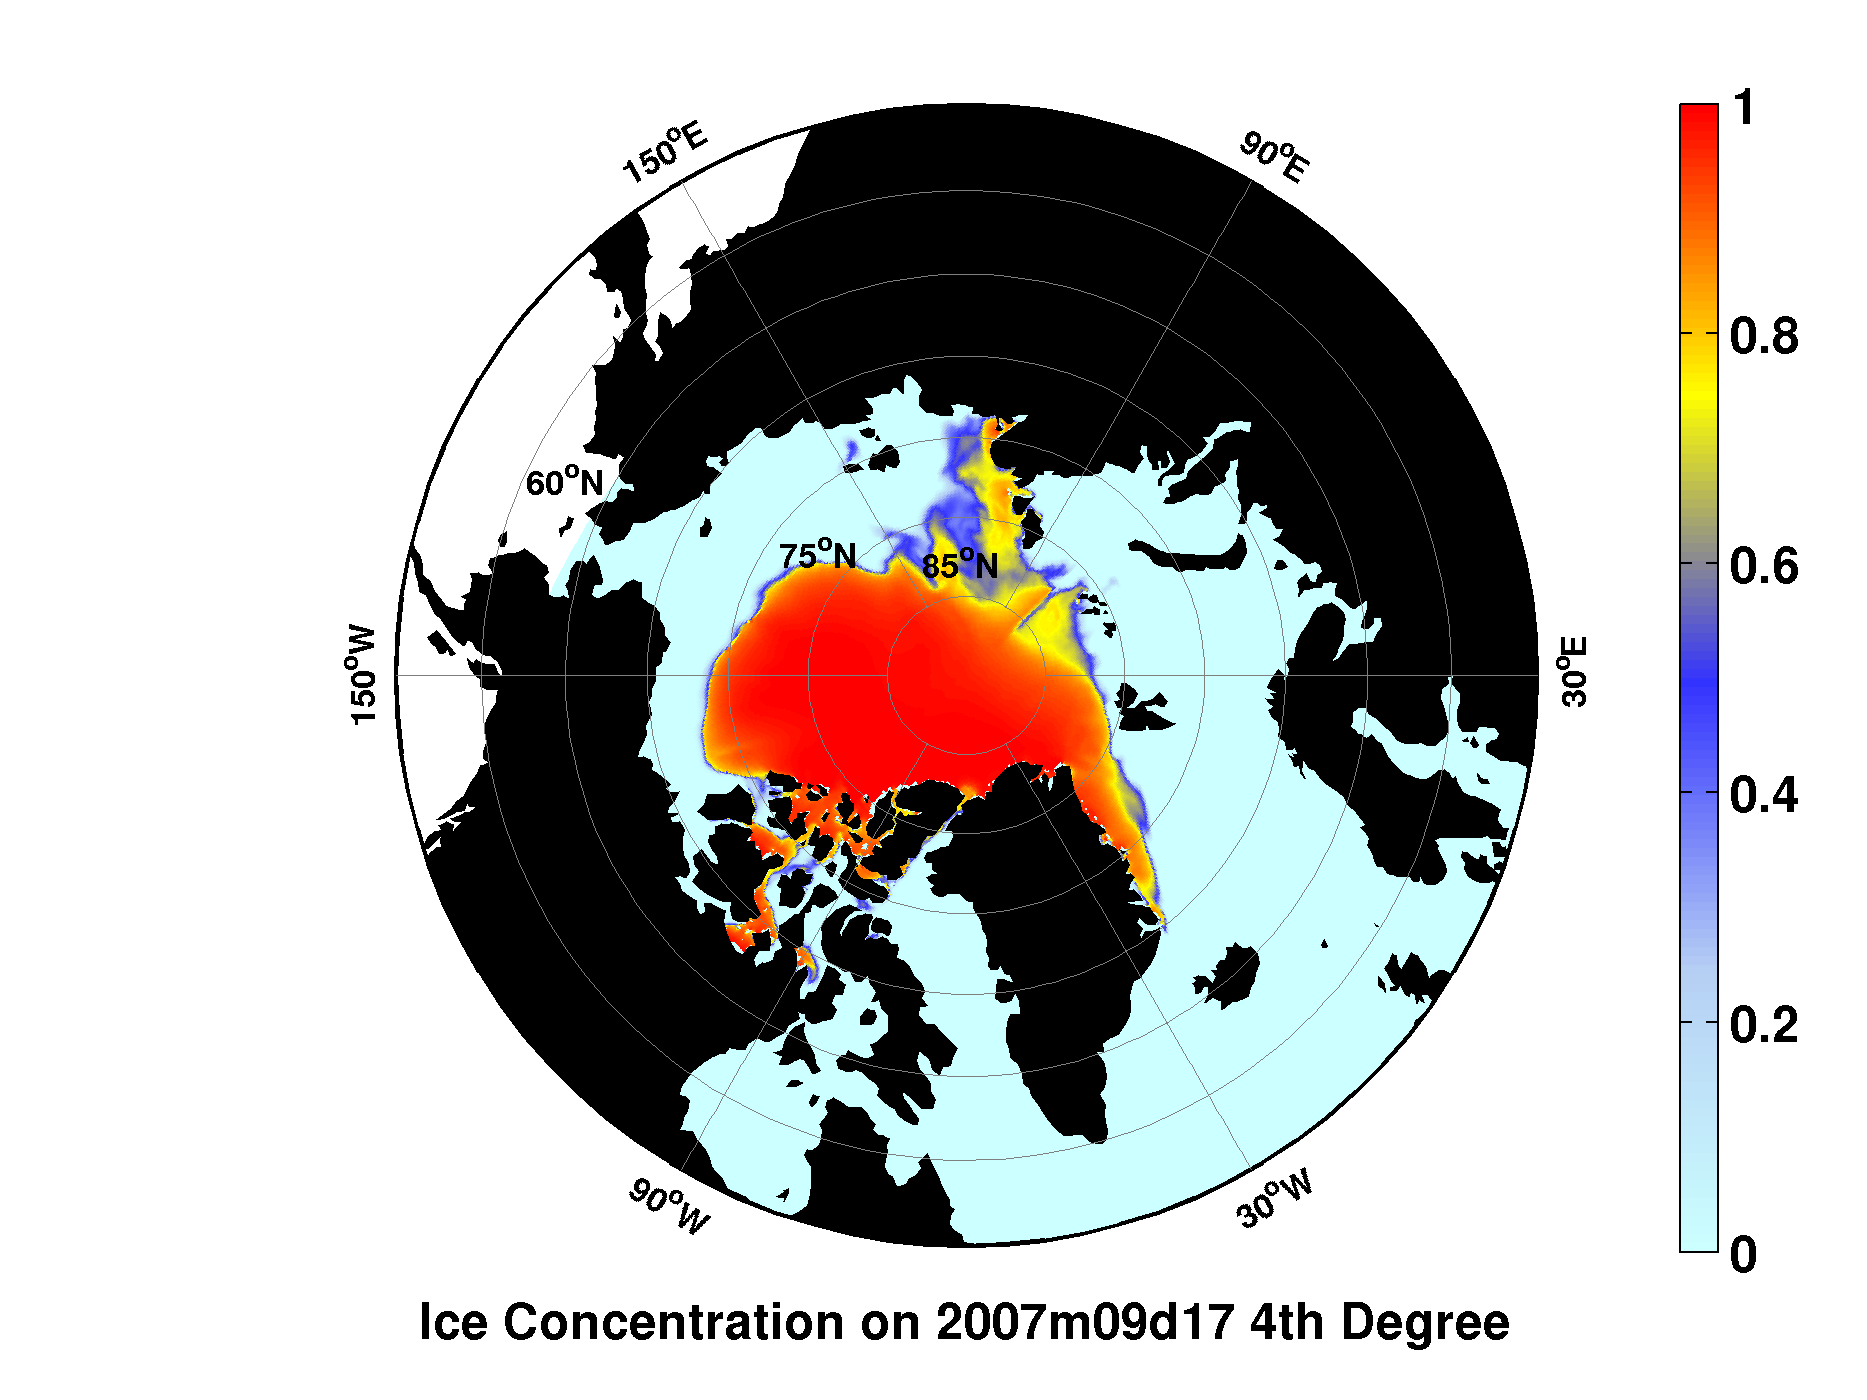
\includegraphics[width=\linewidth]{/home/jingfan/Desktop/Step1/3/Ice_Concentration_2007m09d17_4th_Degree.png}
\end{column}
\begin{column}[t]{0.5\linewidth}
\centering
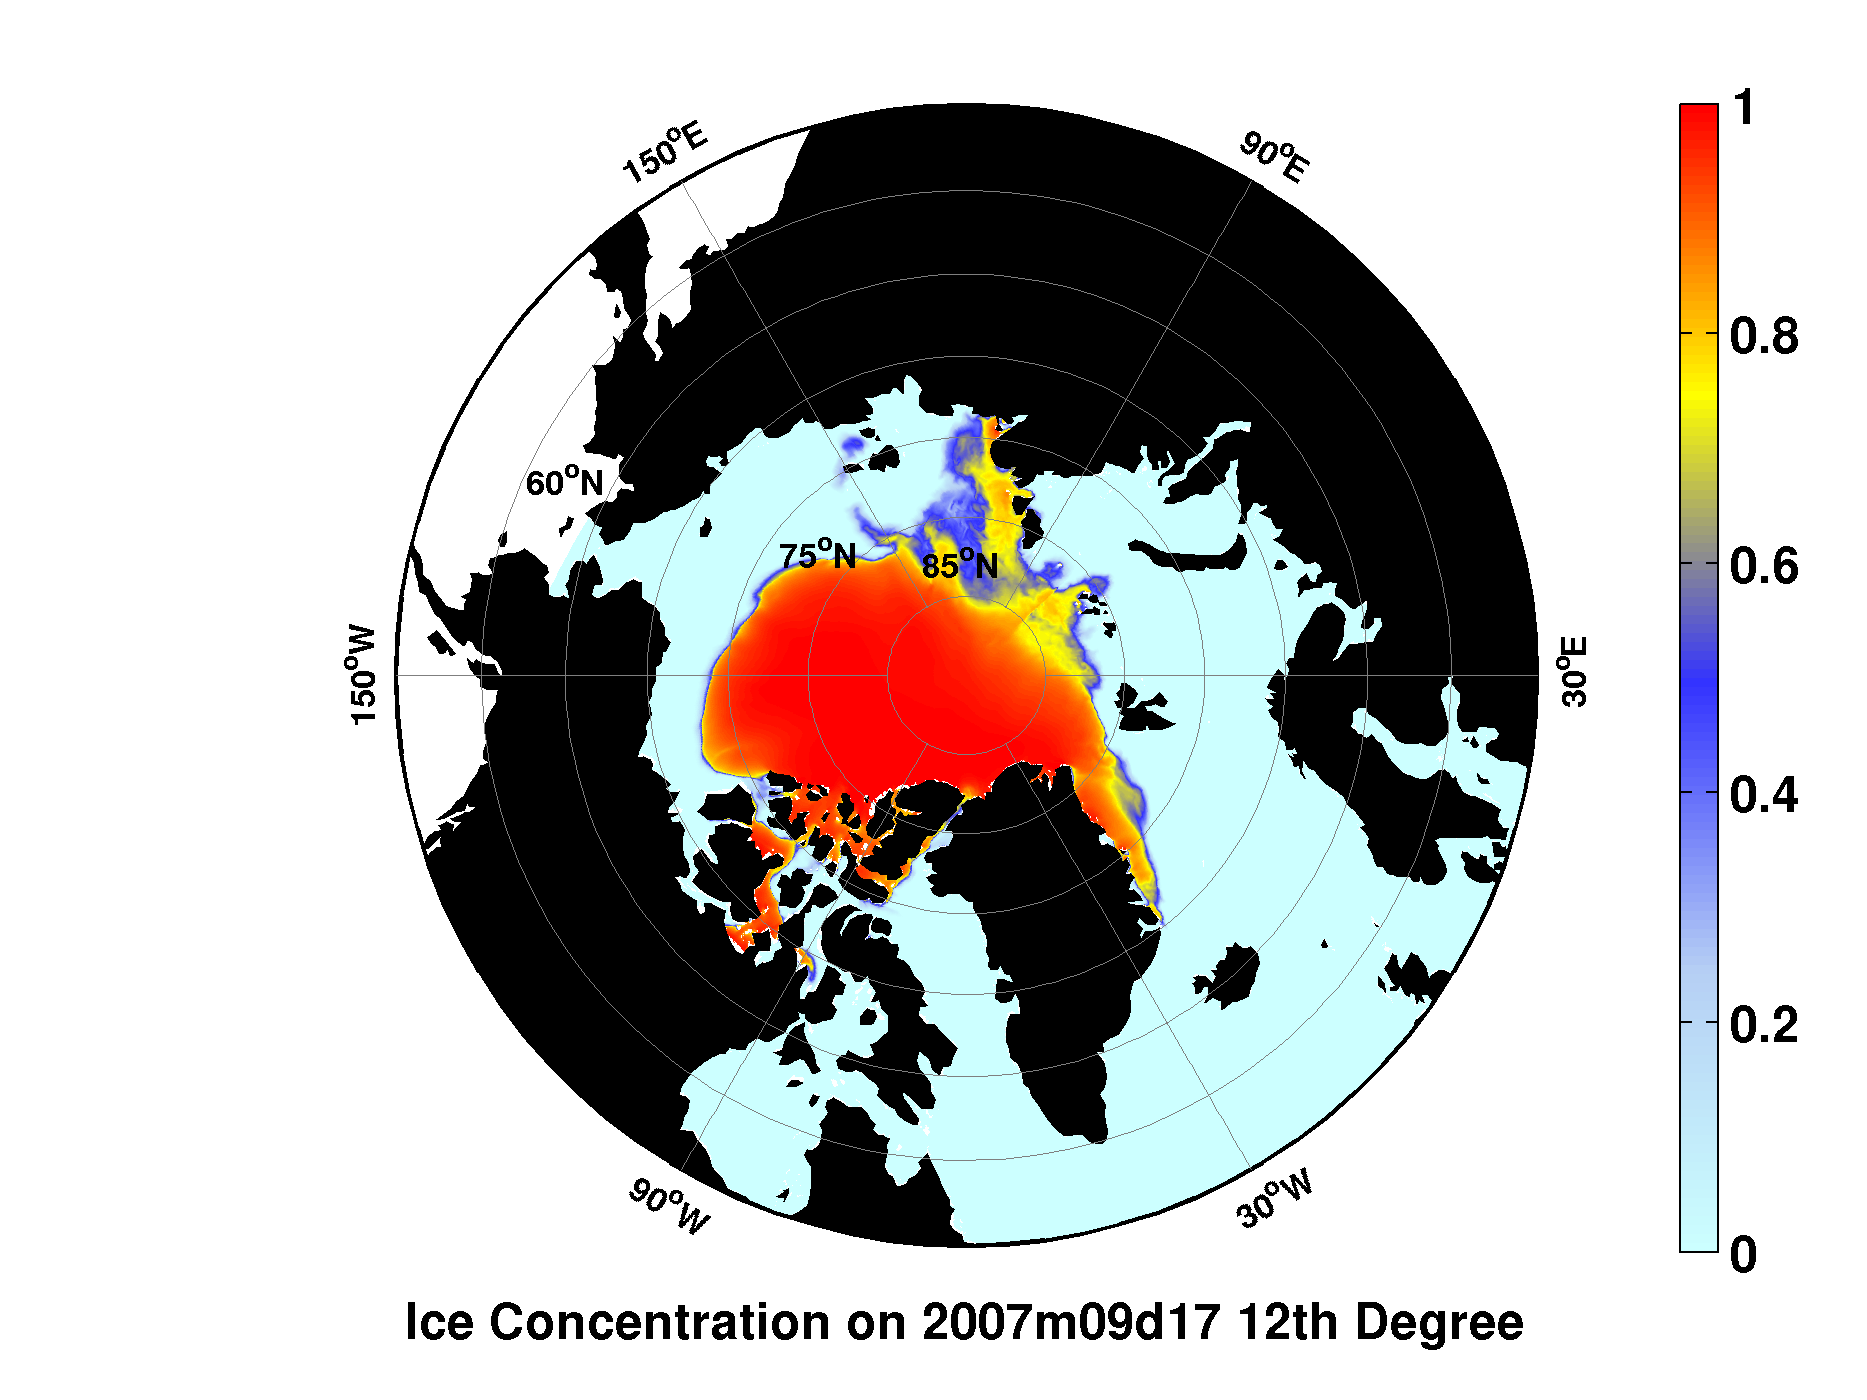
\includegraphics[width=\linewidth]{/home/jingfan/Desktop/Step1/3/Ice_Concentration_2007m09d17_12th_Degree.png}
\end{column}
\end{columns}

\end{frame}

\begin{frame}
\frametitle{Sea-Ice Concentration September 2007 Difference(ANHA12-ANHA4)}

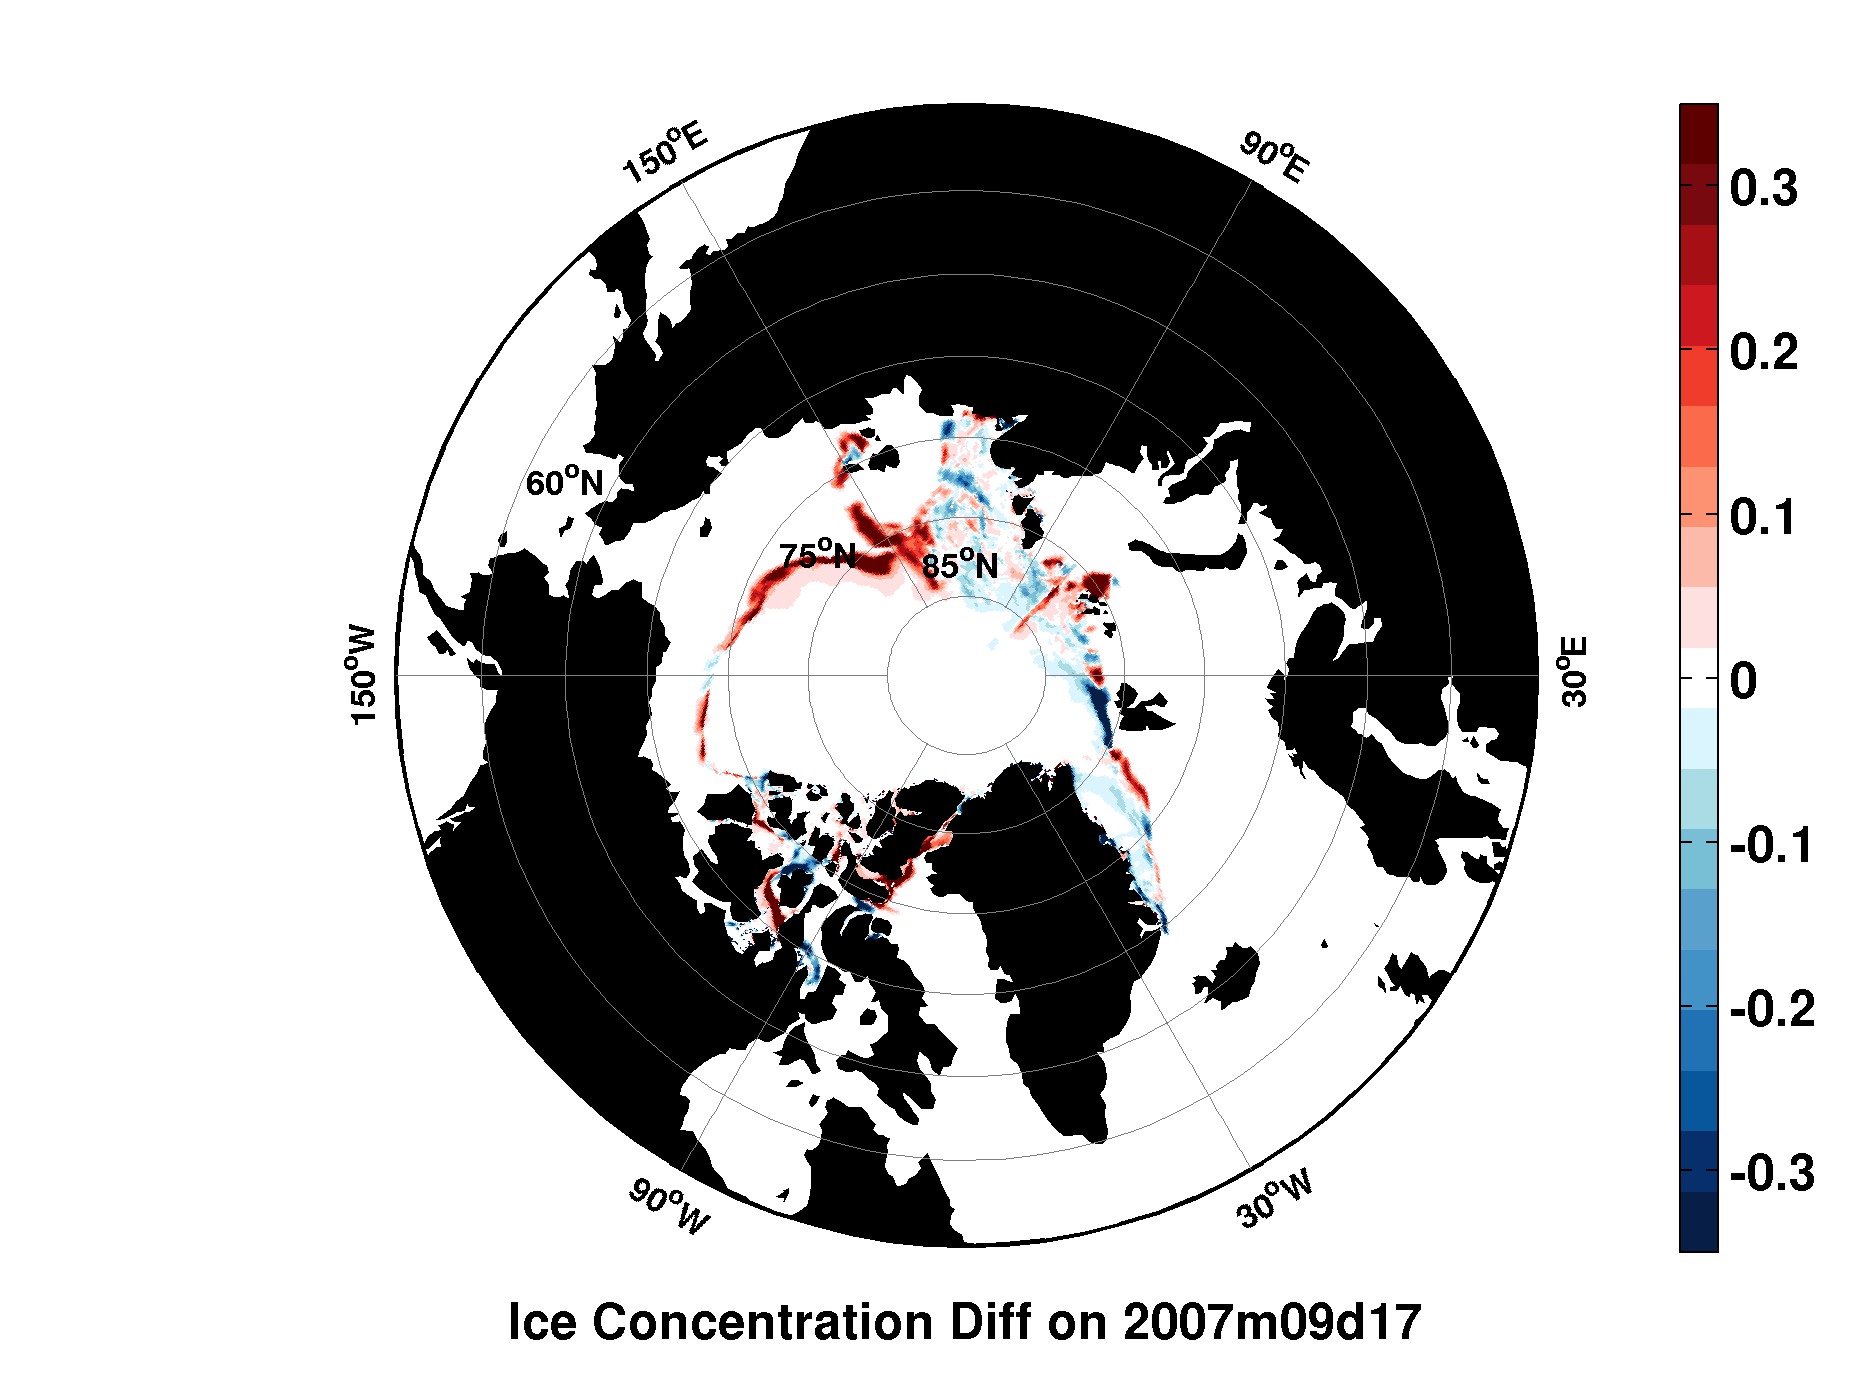
\includegraphics[width=0.9\linewidth]{/home/jingfan/Desktop/Step1/3/Ice_Concentration_Diff_2007m09d17.png}

\end{frame}

\begin{frame}
\frametitle{Sea-Ice Concentration September 2007}

\begin{columns}
\begin{column}[t]{0.5\linewidth}
\centering
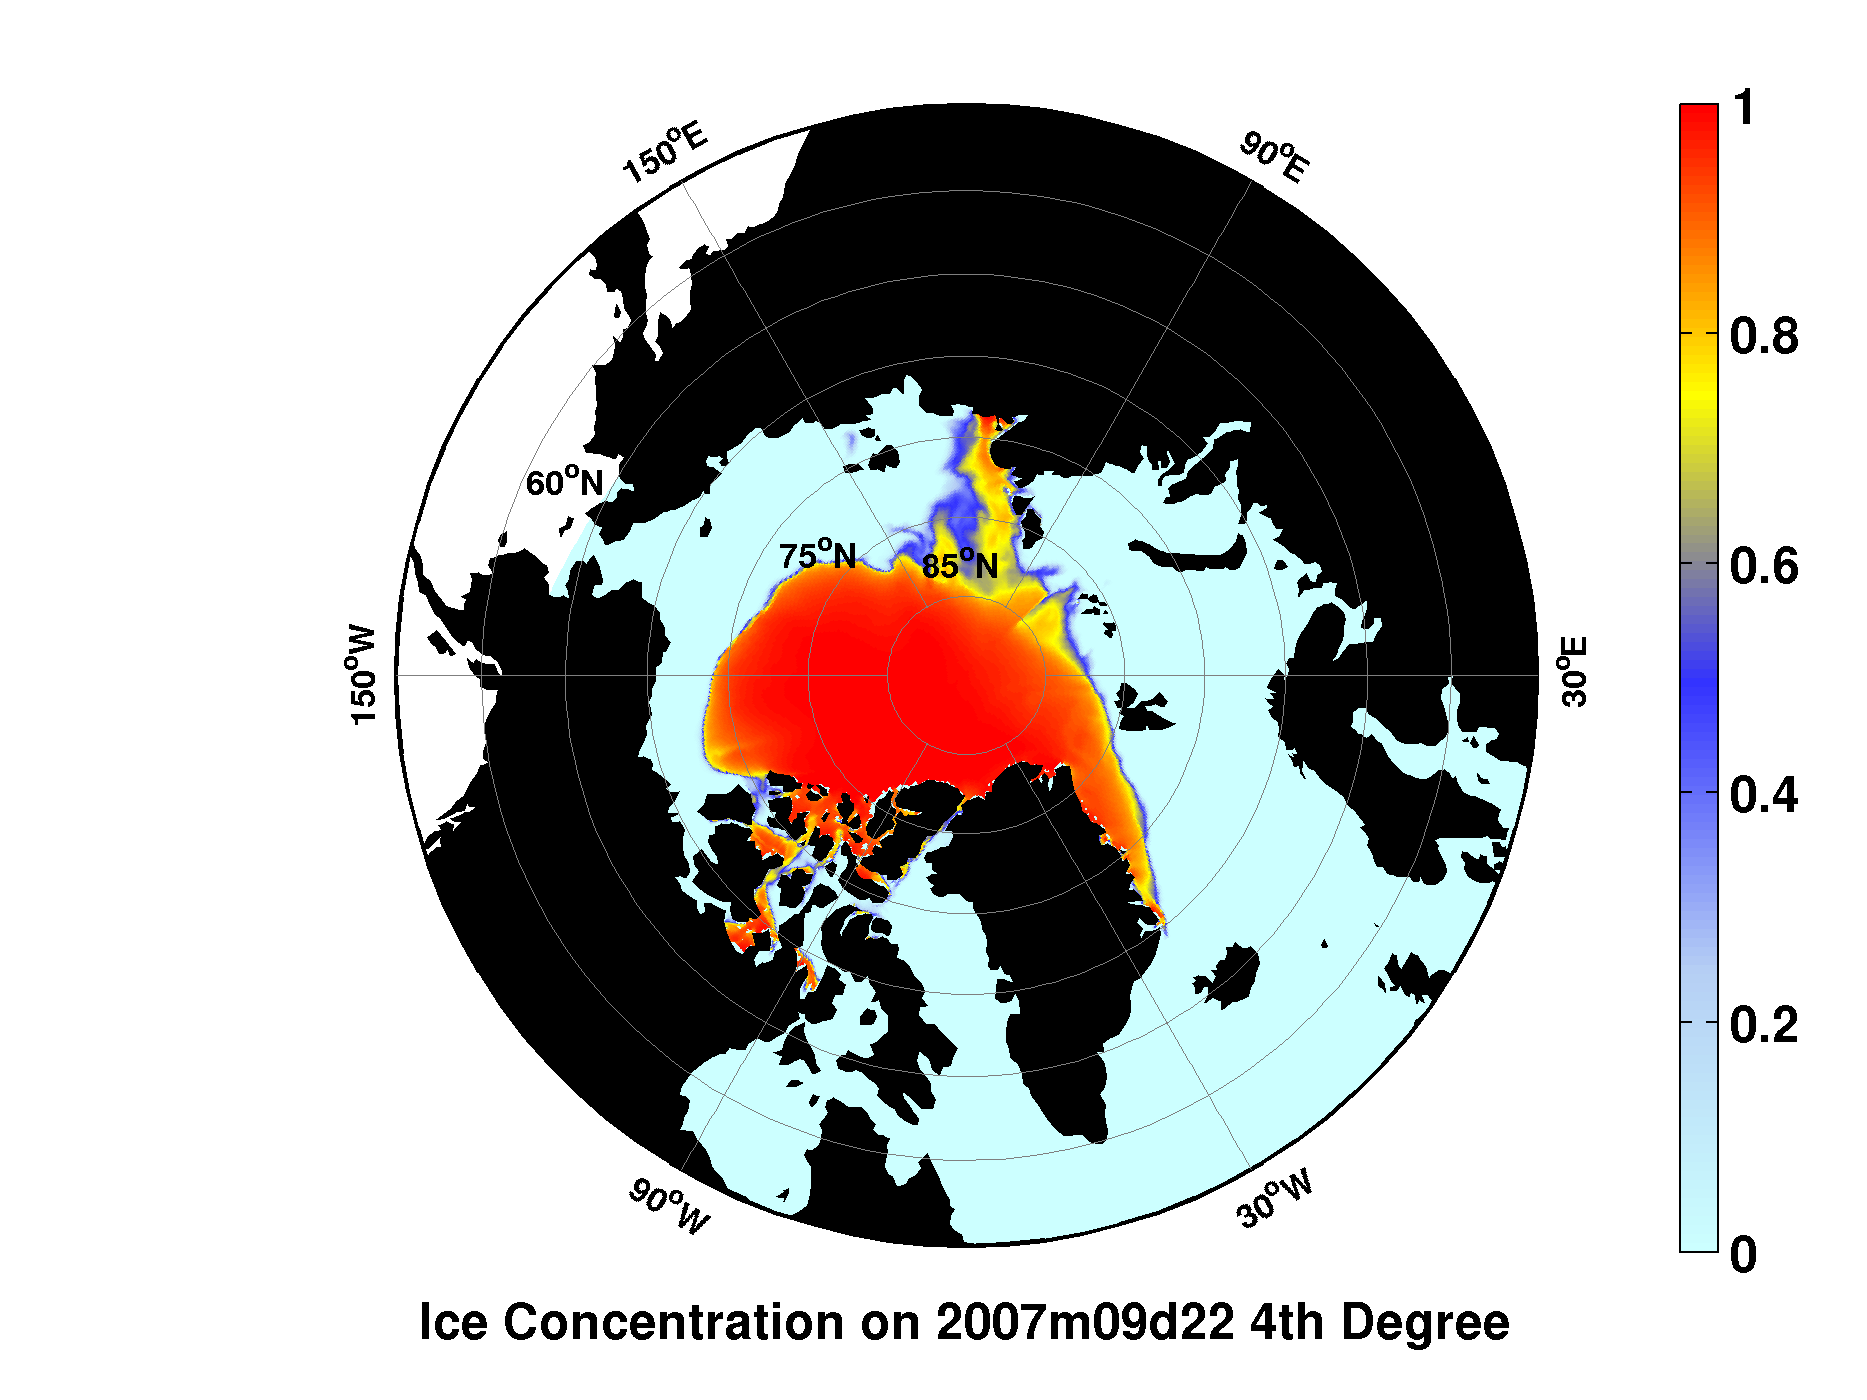
\includegraphics[width=\linewidth]{/home/jingfan/Desktop/Step1/3/Ice_Concentration_2007m09d22_4th_Degree.png}
\end{column}
\begin{column}[t]{0.5\linewidth}
\centering
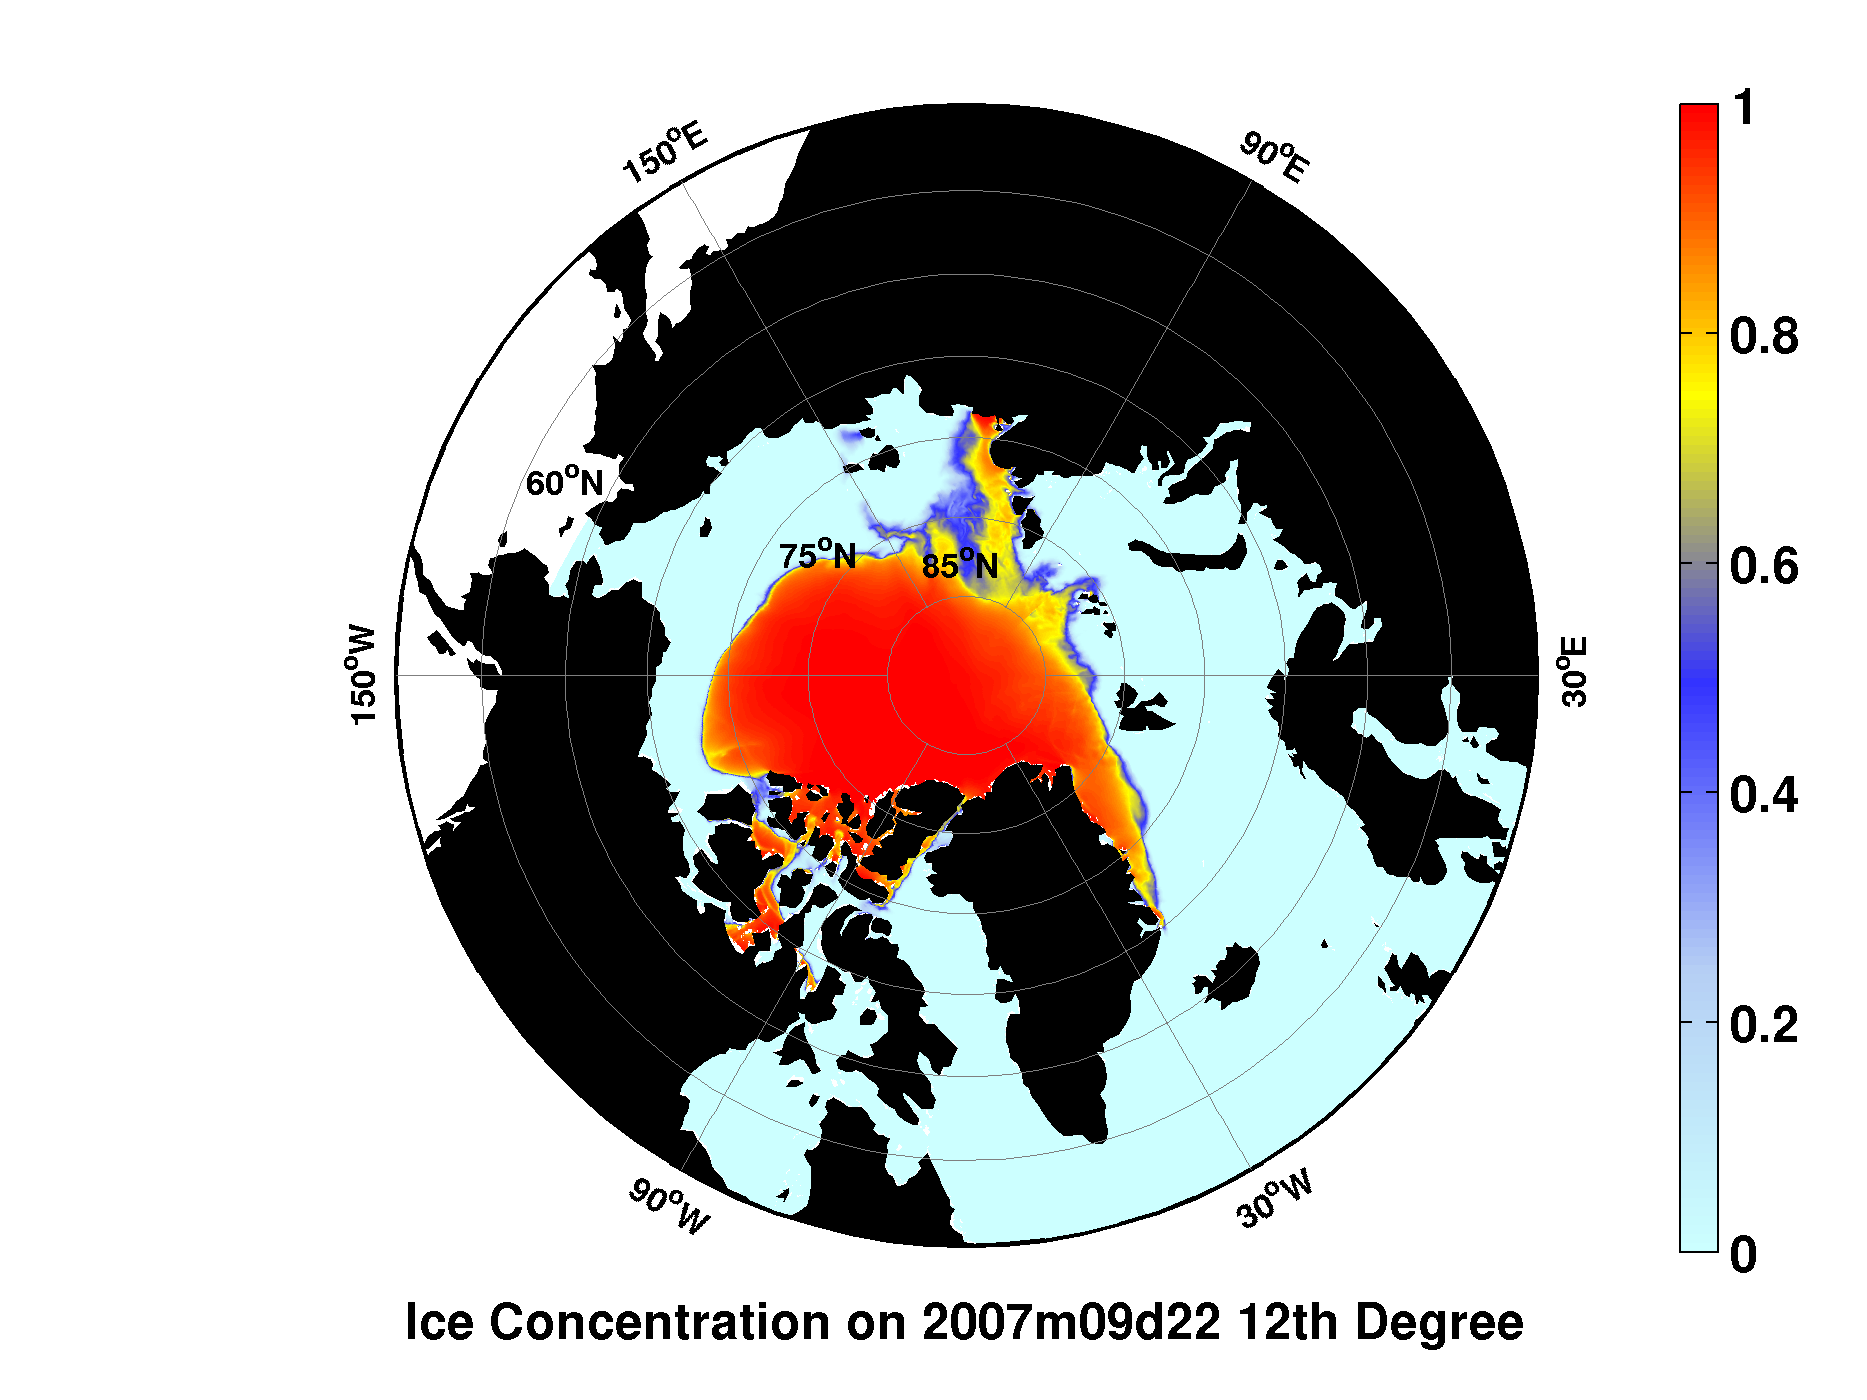
\includegraphics[width=\linewidth]{/home/jingfan/Desktop/Step1/3/Ice_Concentration_2007m09d22_12th_Degree.png}
\end{column}
\end{columns}

\end{frame}

\begin{frame}
\frametitle{Sea-Ice Concentration September 2007 Difference(ANHA12-ANHA4)}

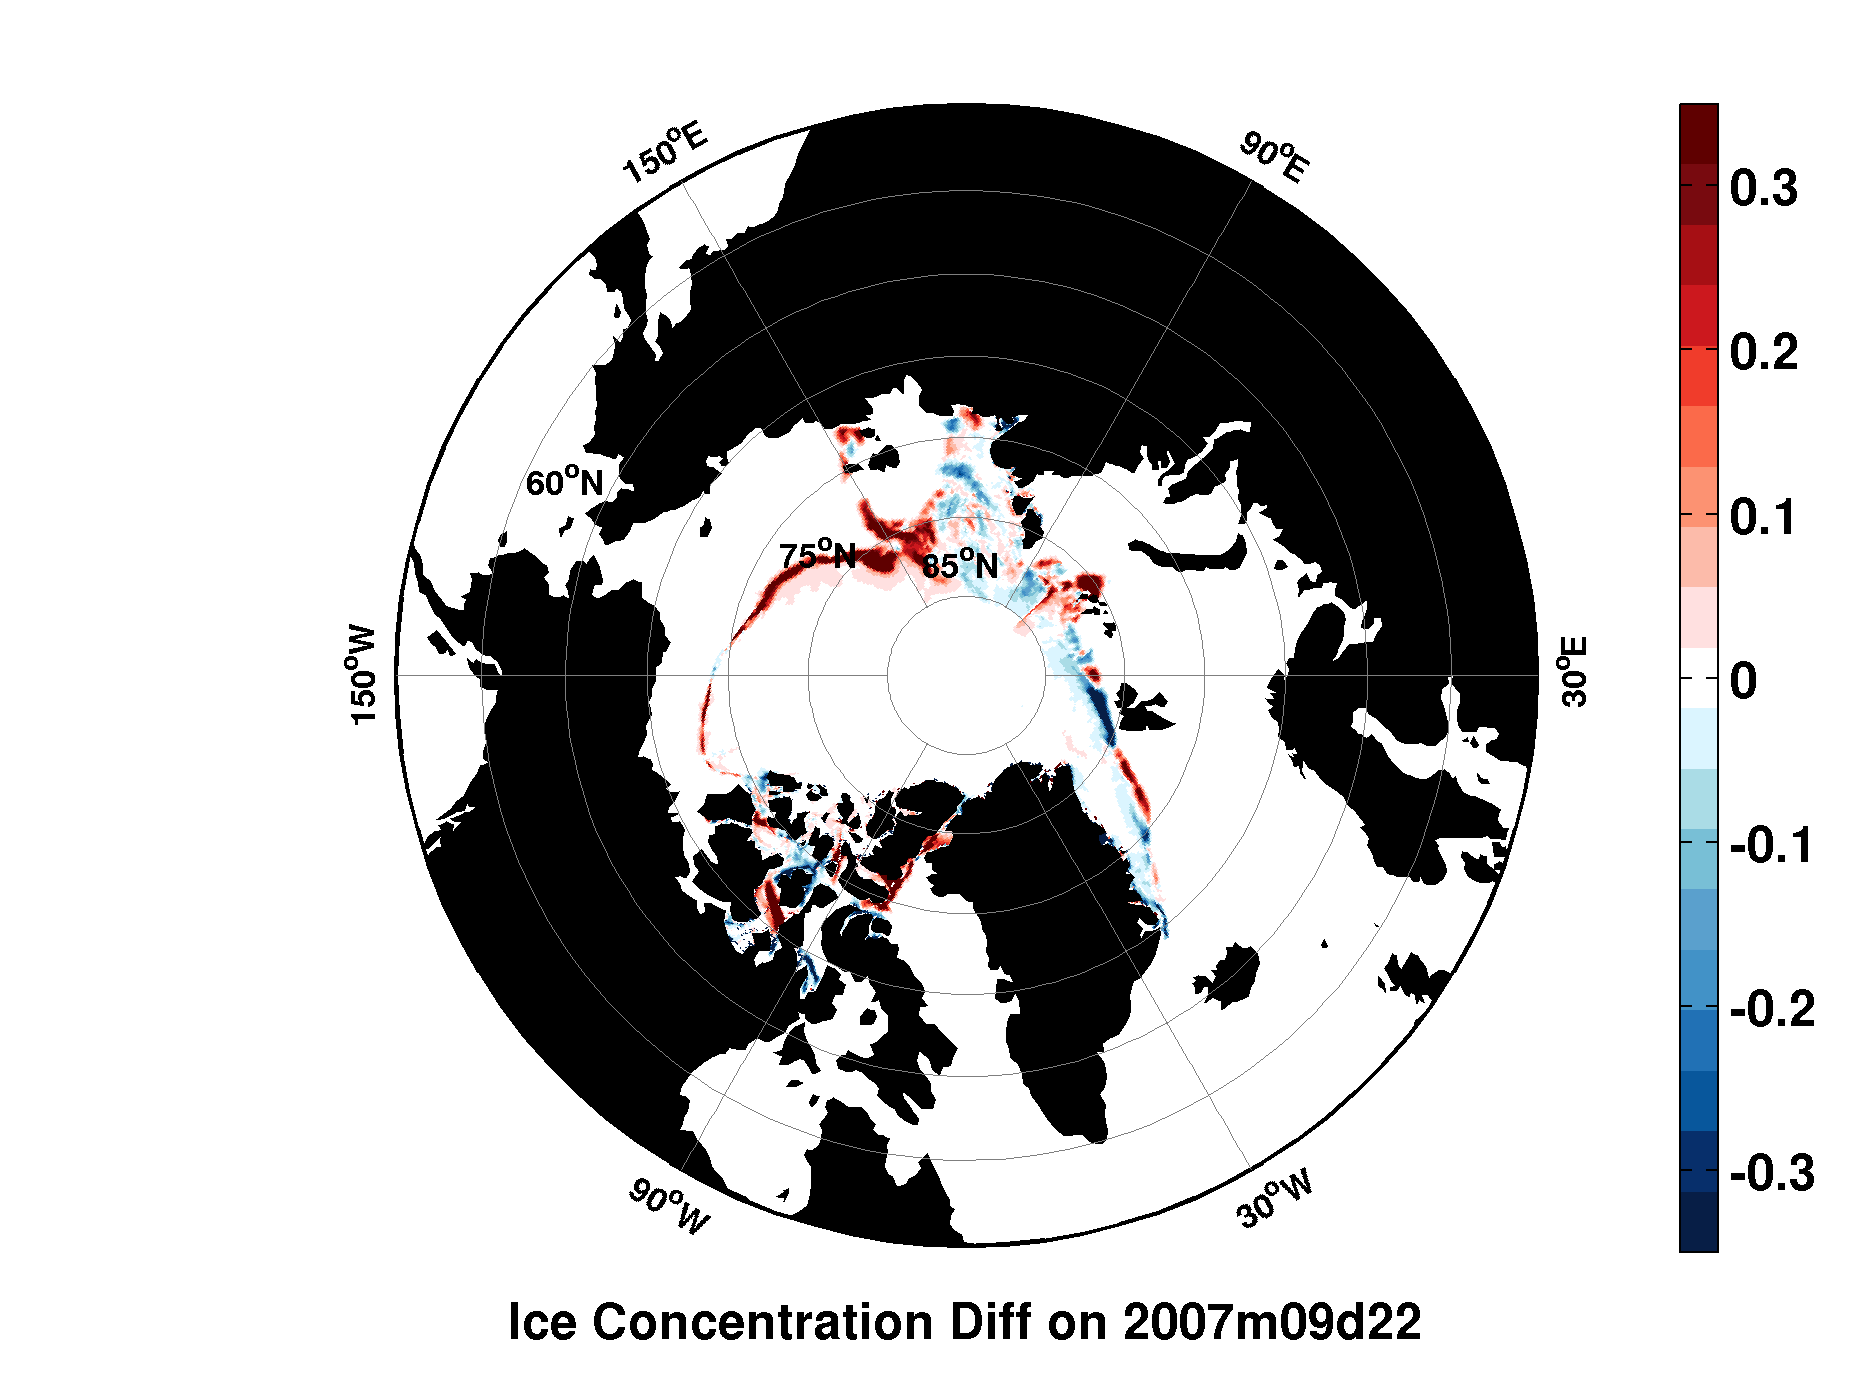
\includegraphics[width=0.9\linewidth]{/home/jingfan/Desktop/Step1/3/Ice_Concentration_Diff_2007m09d22.png}

\end{frame}

\begin{frame}
\frametitle{Sea-Ice Concentration September 2007}

\begin{columns}
\begin{column}[t]{0.5\linewidth}
\centering
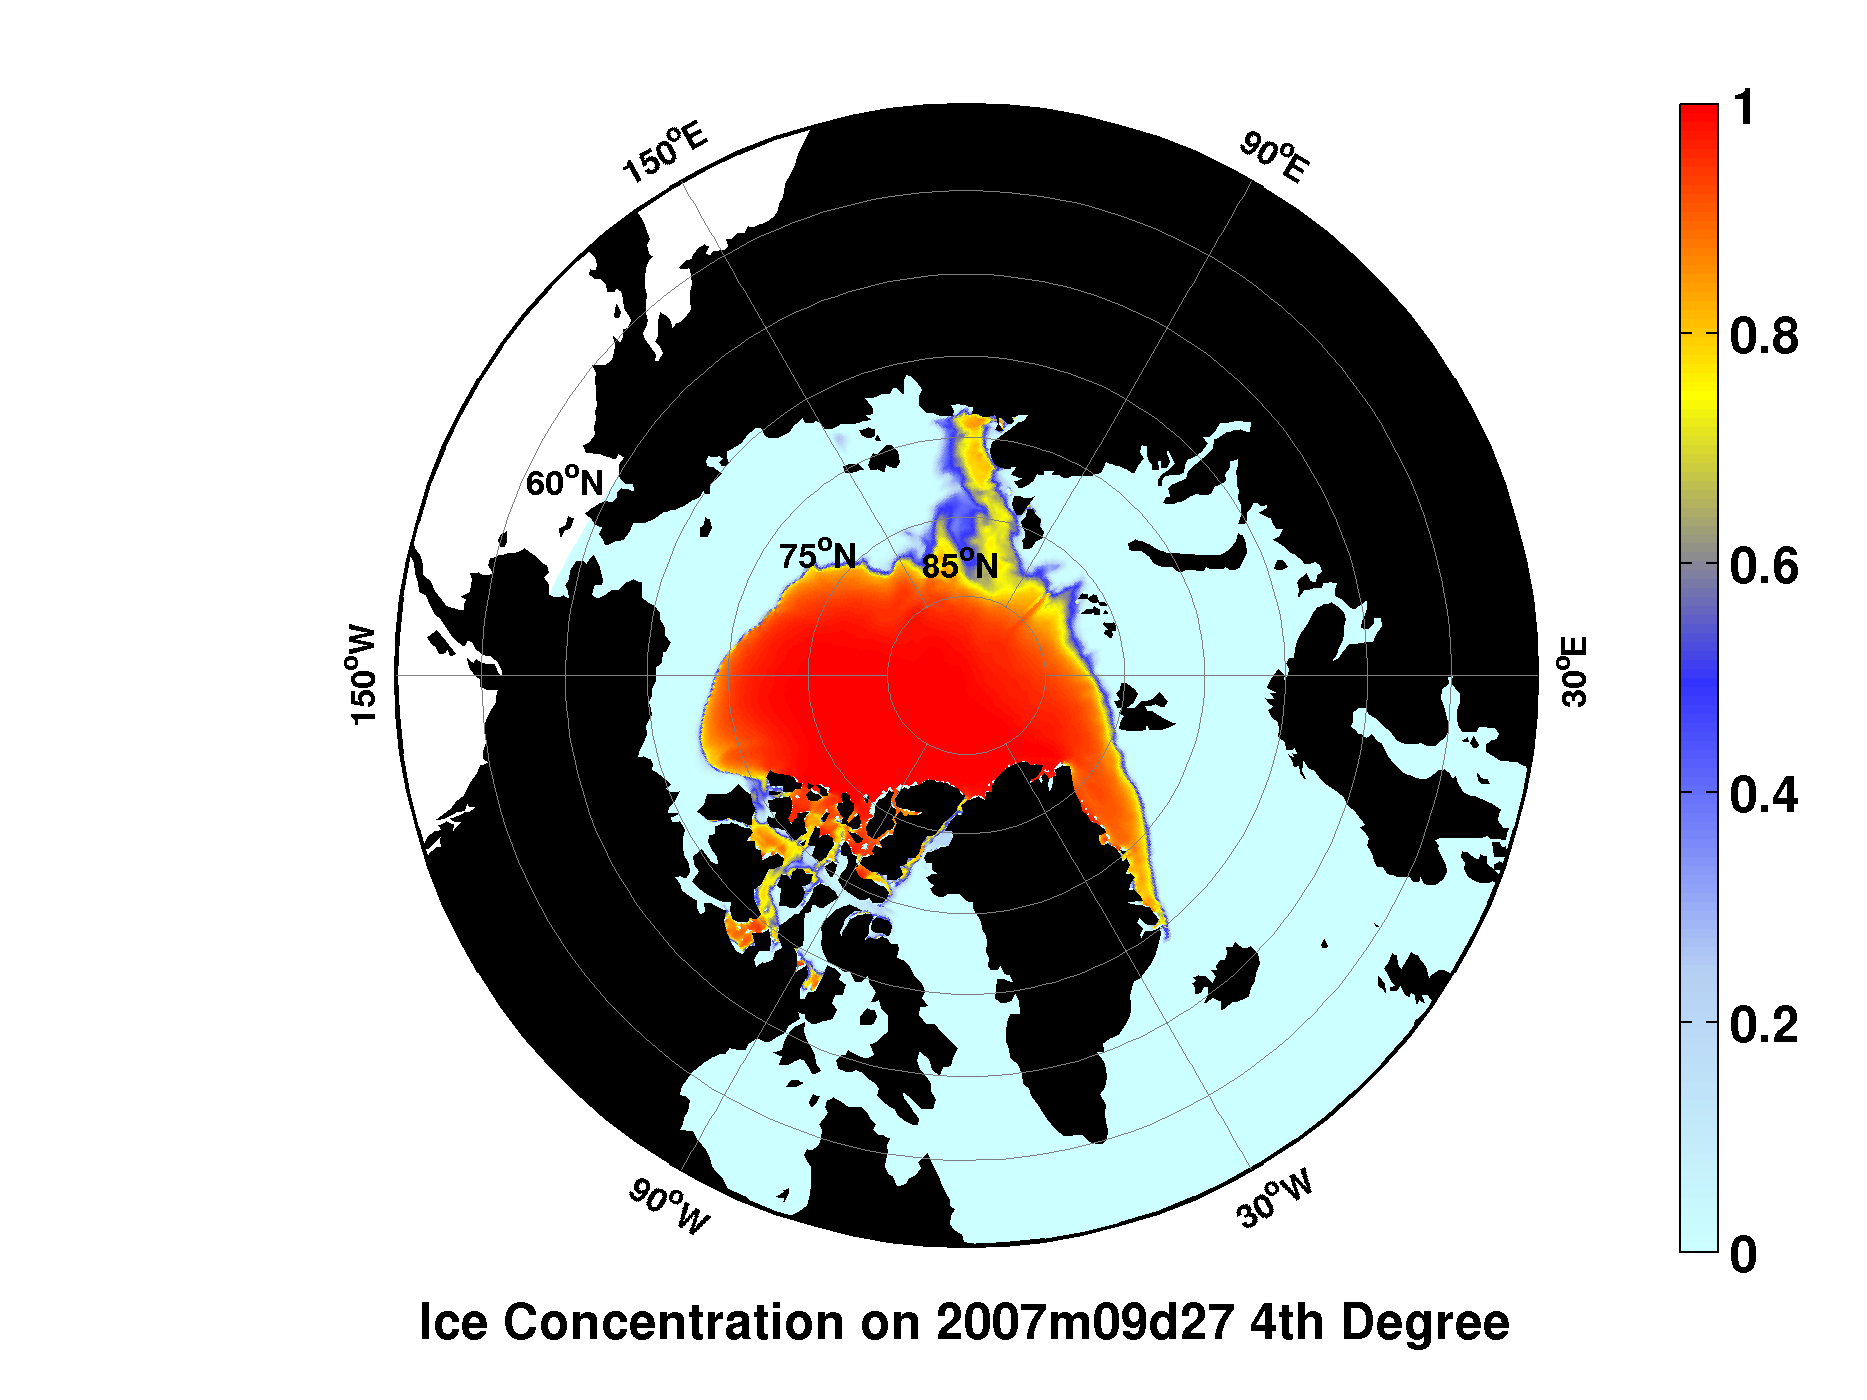
\includegraphics[width=\linewidth]{/home/jingfan/Desktop/Step1/3/Ice_Concentration_2007m09d27_4th_Degree.png}
\end{column}
\begin{column}[t]{0.5\linewidth}
\centering
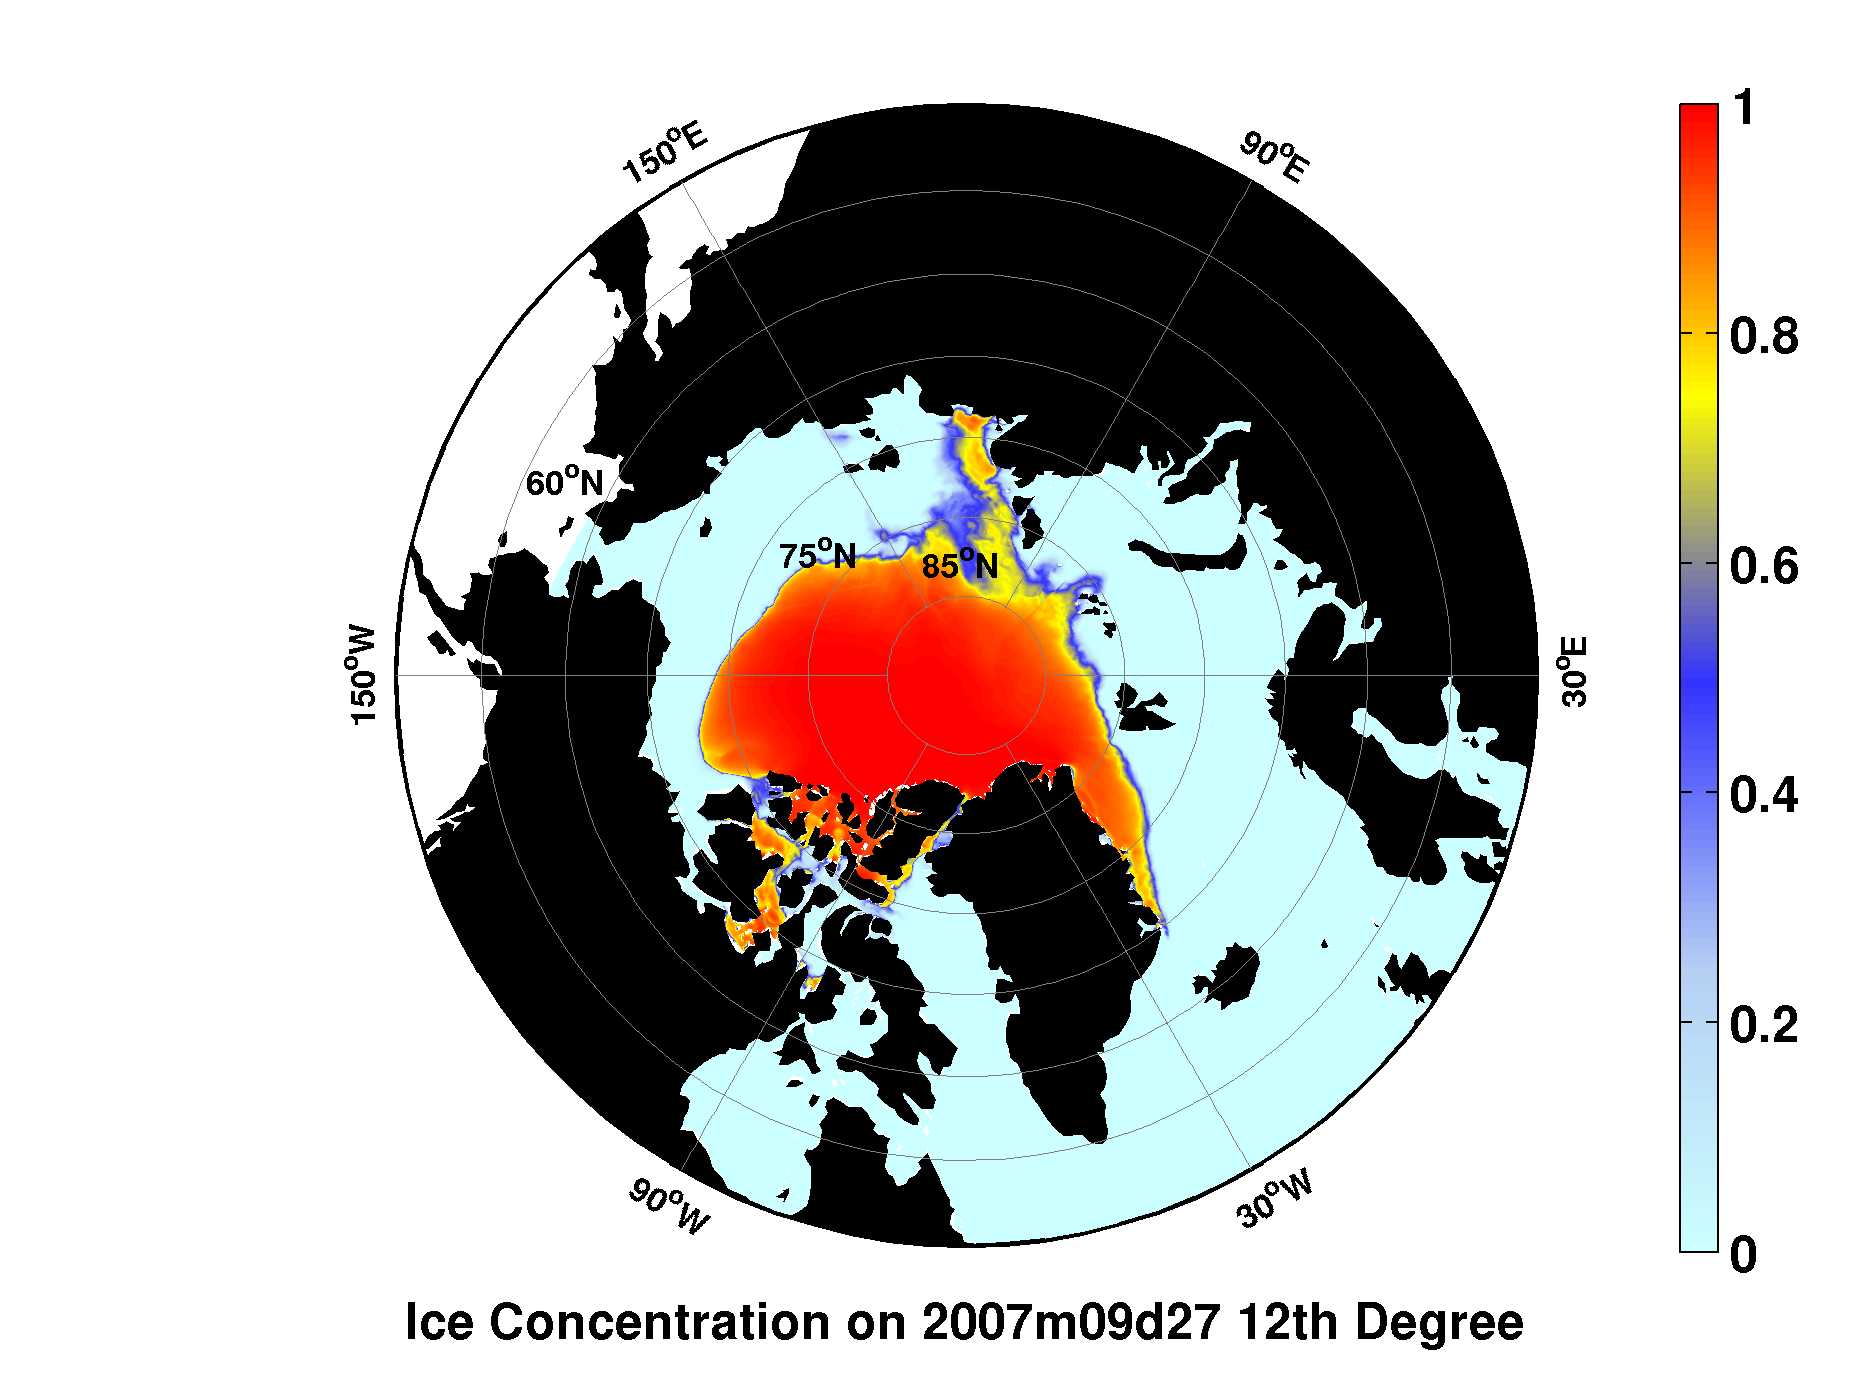
\includegraphics[width=\linewidth]{/home/jingfan/Desktop/Step1/3/Ice_Concentration_2007m09d27_12th_Degree.png}
\end{column}
\end{columns}

\end{frame}

\begin{frame}
\frametitle{Sea-Ice Concentration September 2007 Difference(ANHA12-ANHA4)}

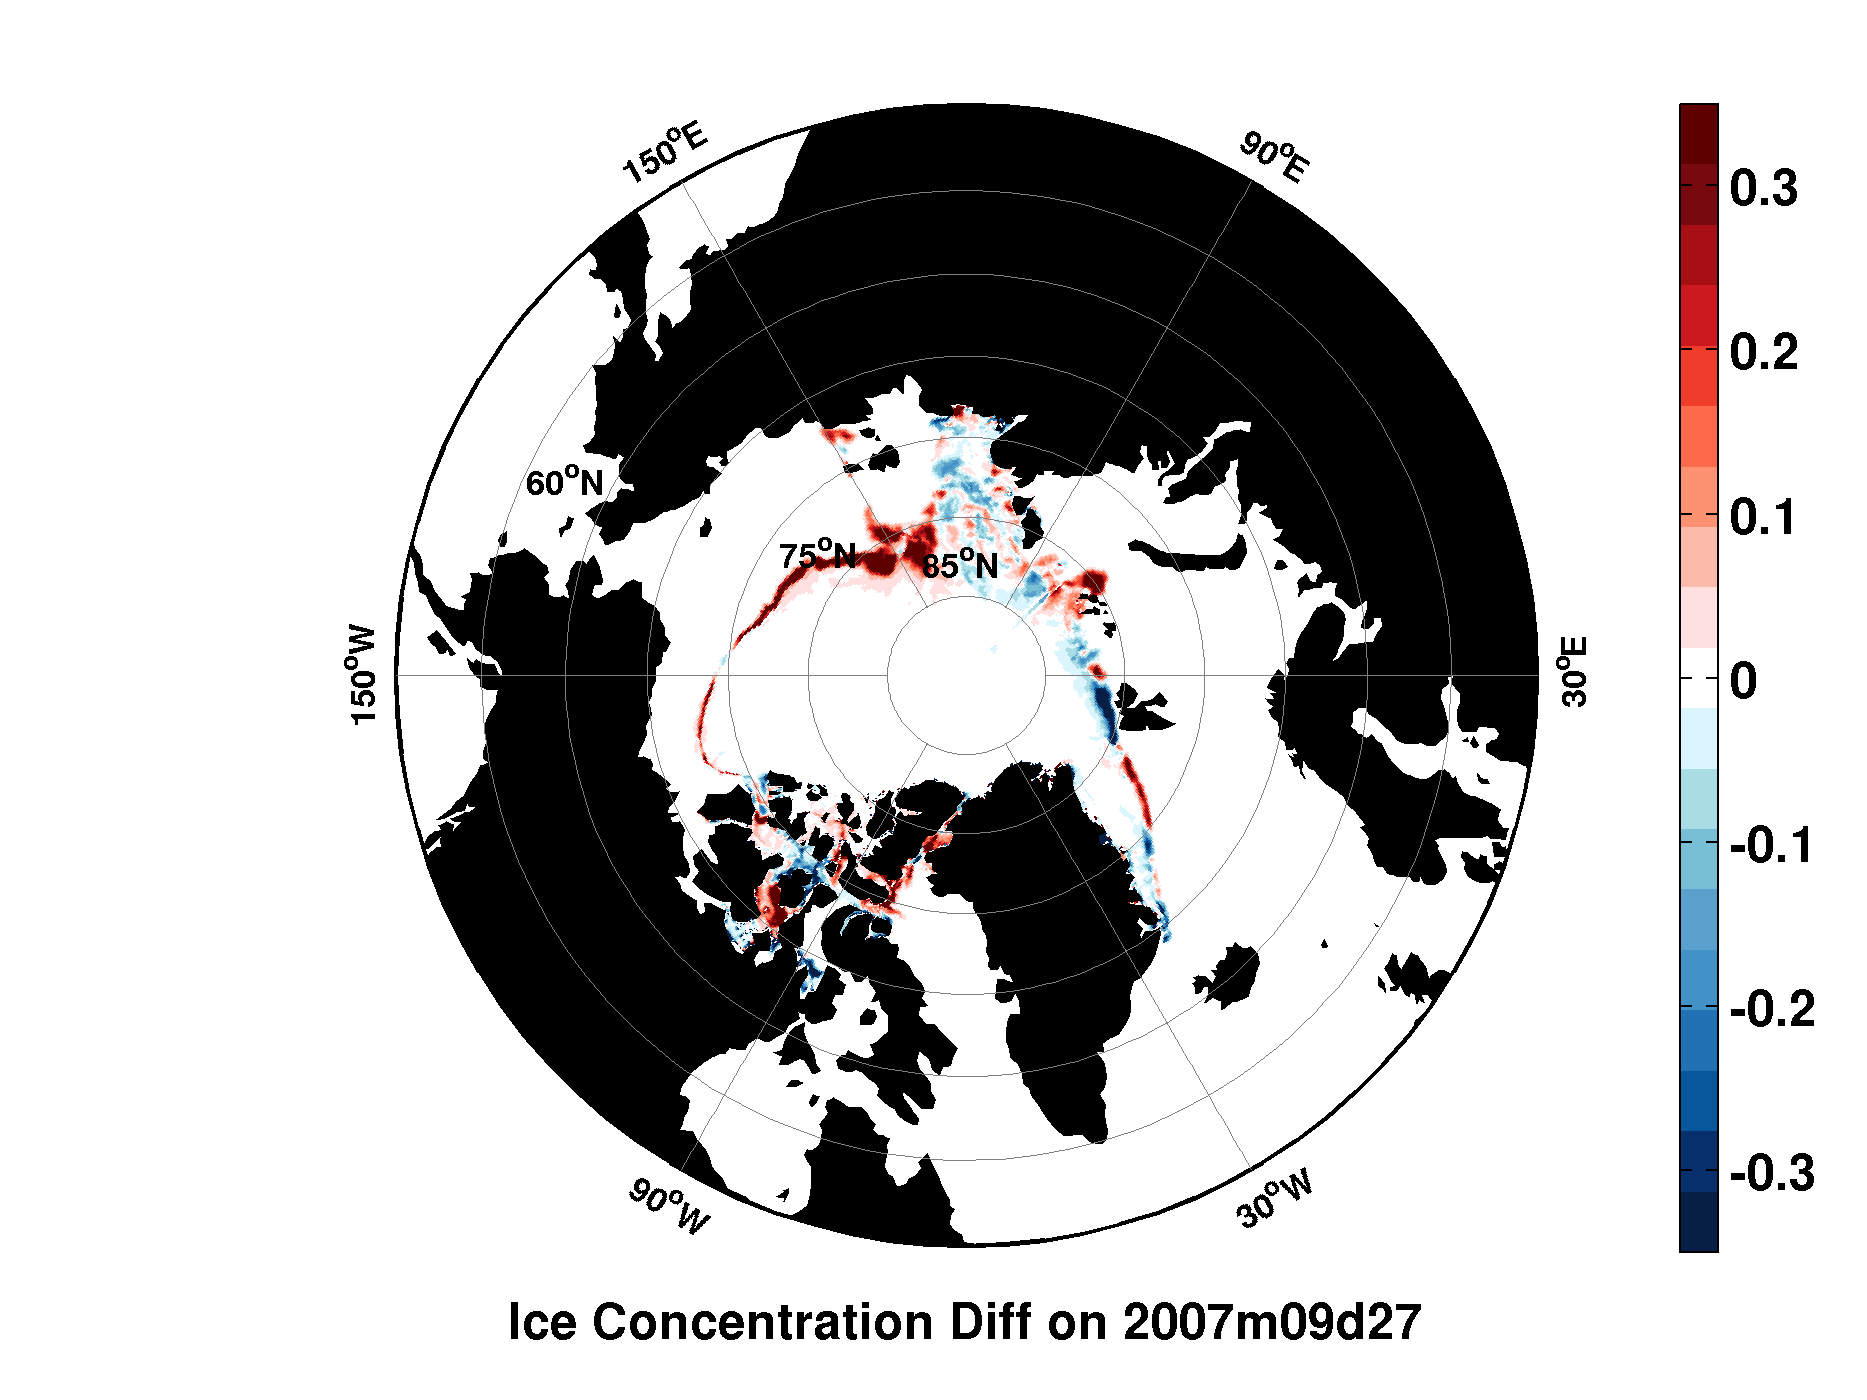
\includegraphics[width=0.9\linewidth]{/home/jingfan/Desktop/Step1/3/Ice_Concentration_Diff_2007m09d27.png}

\end{frame}

%%%%%%%%%%%%%%%%%%%%%%%%%%%%%%%%%%%%%%%%%%%%%%%%%%%%%%%%%%%%
%% Sea-Ice Thickness Analysis
\section{Sea-Ice Thickness Analysis}
\begin{frame}
\frametitle{Sea-Ice Thickness Analysis}

In the region north of 55N: 

\begin{itemize}

\item Mean Sea-Ice Thickness over 2003-2008 for each run for March and September, with difference plots
\item Sea-Ice Thickness Standard Deviation over 2003-2008 for each run for March and September, with difference plots
\item Sea-Ice Thickness for September 2007, with difference plots

\end{itemize}

\end{frame}

%%%%%%%%%%%%%%%%%%%%%%%%%%%%%%%%%%%%%%%%%%%%%%%%%%%%%%%%%%%%%%
\begin{frame}
\frametitle{Mean Sea-Ice Thickness}
I calculate the mean ice thickness based on the data of every single day in a specific month from 2003-2008. 
\end{frame}

\begin{frame}
\frametitle{Mean Sea-Ice Thickness}

\begin{columns}
\begin{column}[t]{0.5\linewidth}
\centering
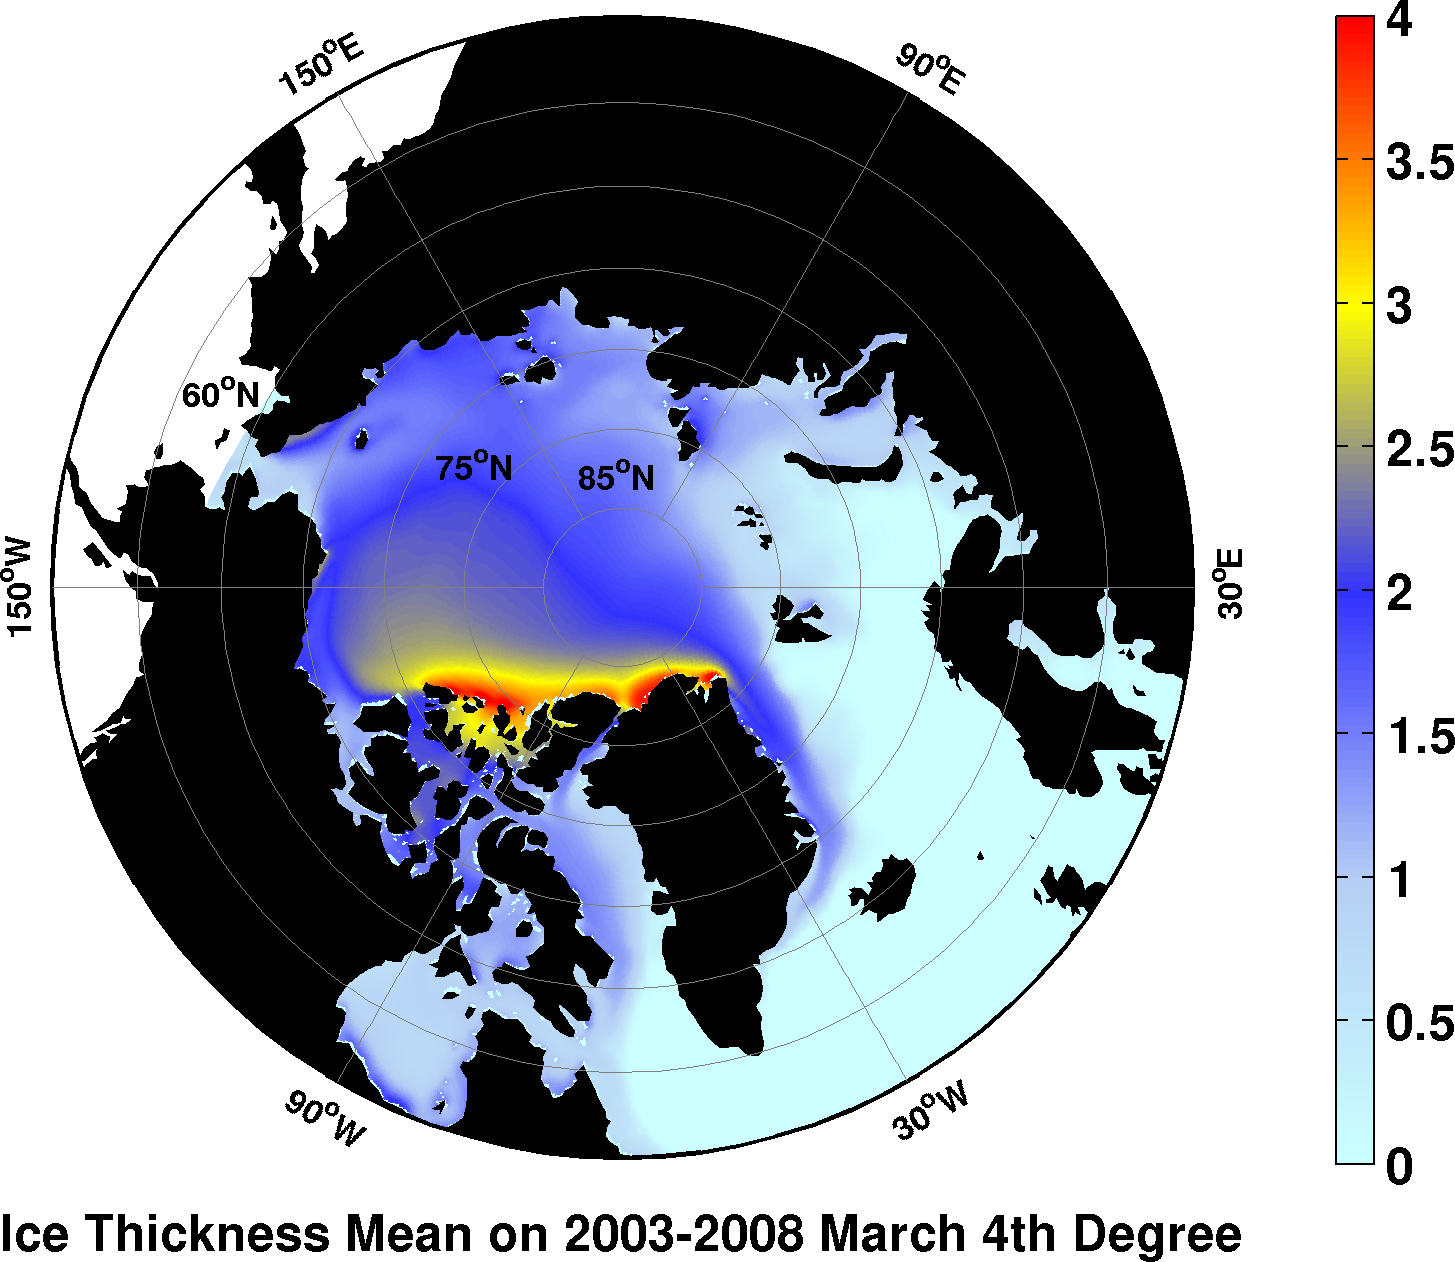
\includegraphics[width=\linewidth]{/home/jingfan/Desktop/Step1/1/Ice_Thickness_mean_2003-2008_March_4th_Degree.png}
\end{column}
\begin{column}[t]{0.5\linewidth}
\centering
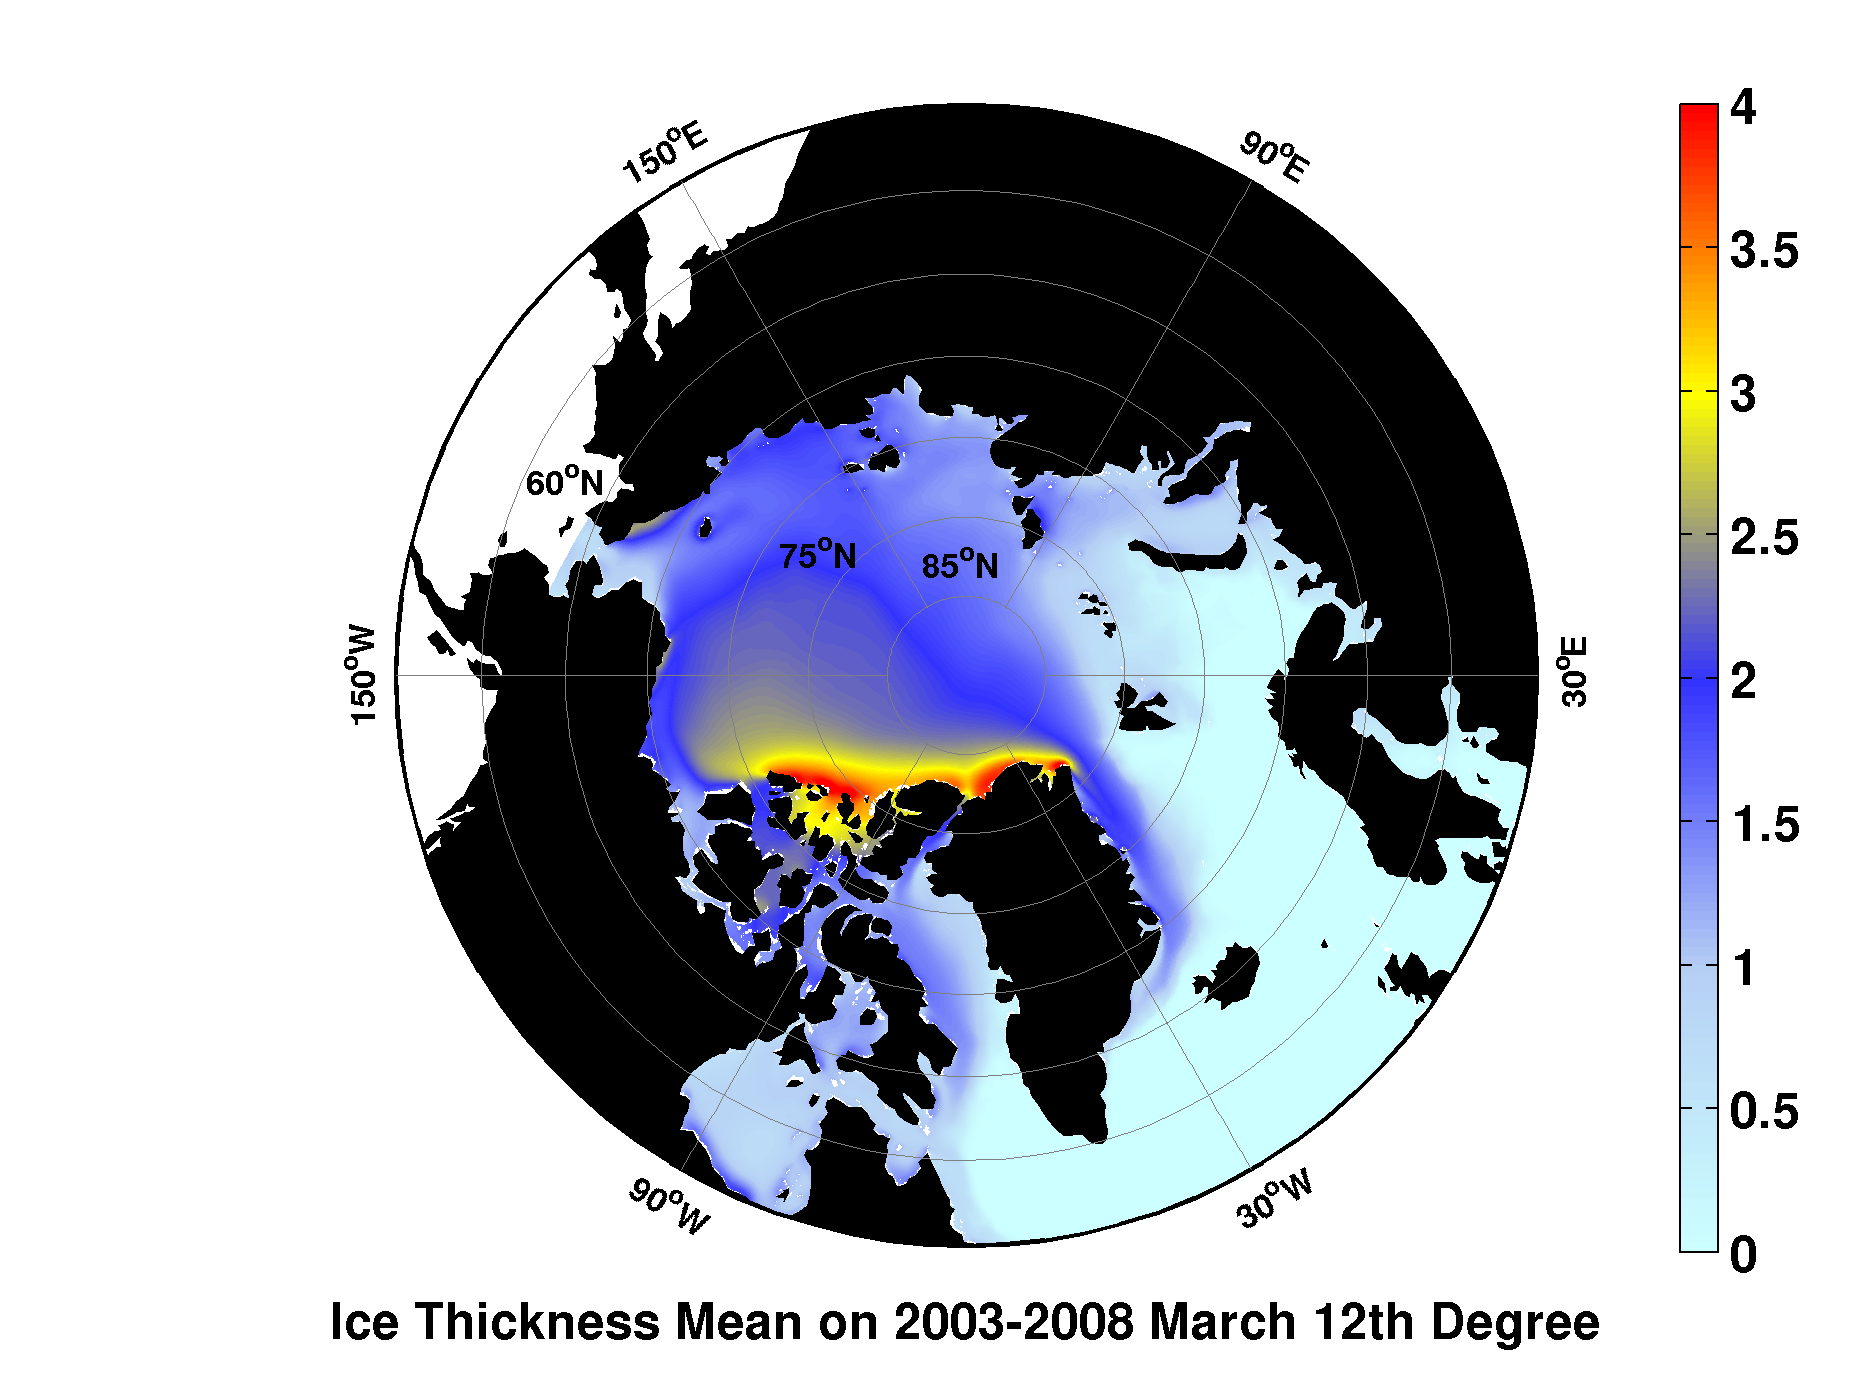
\includegraphics[width=\linewidth]{/home/jingfan/Desktop/Step1/1/Ice_Thickness_mean_2003-2008_March_12th_Degree.png}
\end{column}
\end{columns}

\end{frame}

\begin{frame}
\frametitle{Mean Sea-Ice Thickness Difference(ANHA12-ANHA4)}

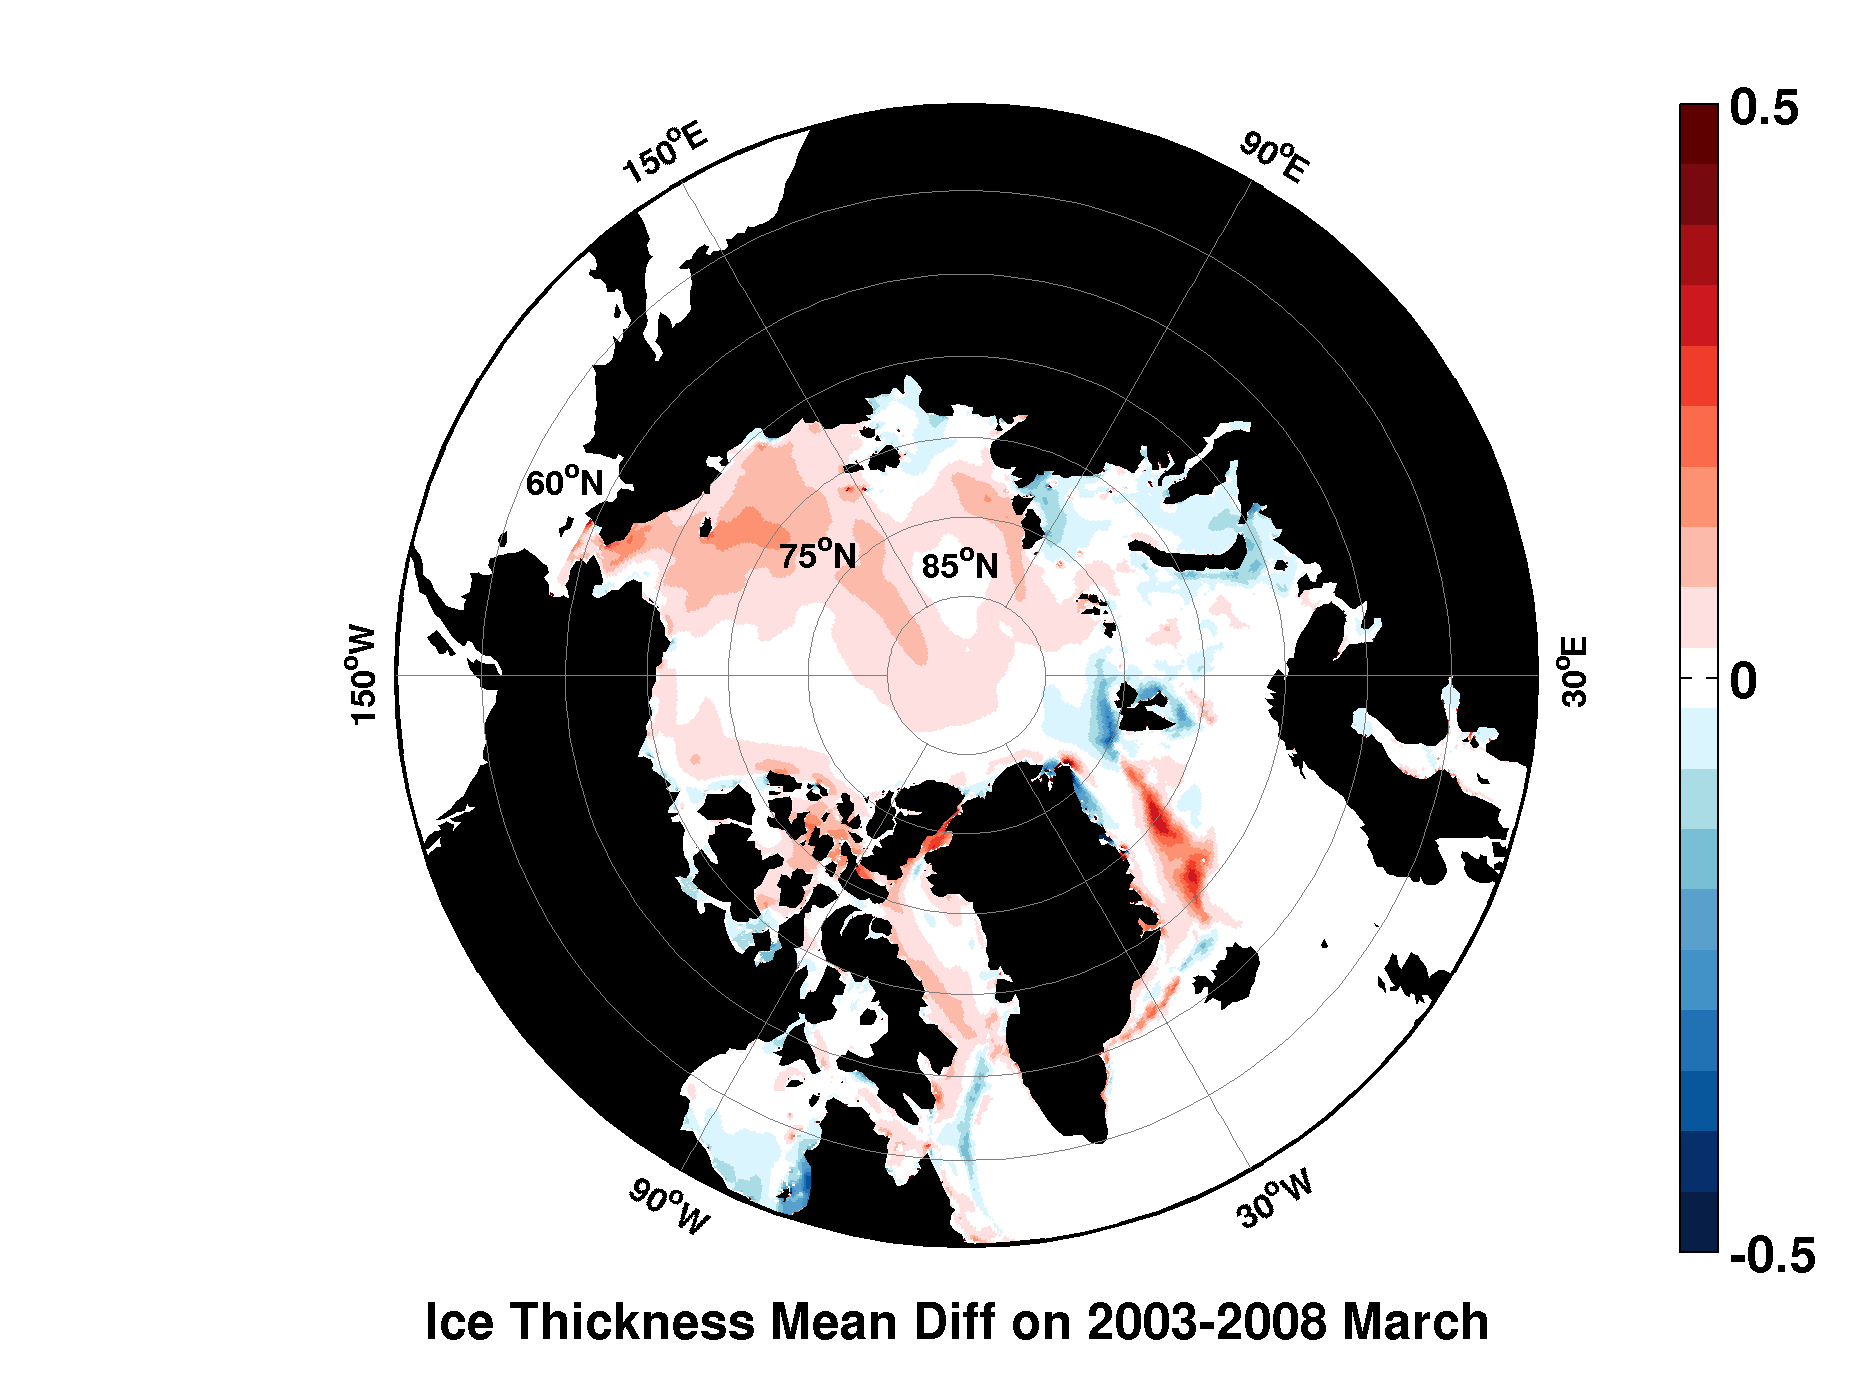
\includegraphics[width=0.9\linewidth]{/home/jingfan/Desktop/Step1/1/Ice_Thickness_mean_Diff_2003-2008_March.png}

\end{frame}

\begin{frame}
\frametitle{Mean Sea-Ice Thickness}

\begin{columns}
\begin{column}[t]{0.5\linewidth}
\centering
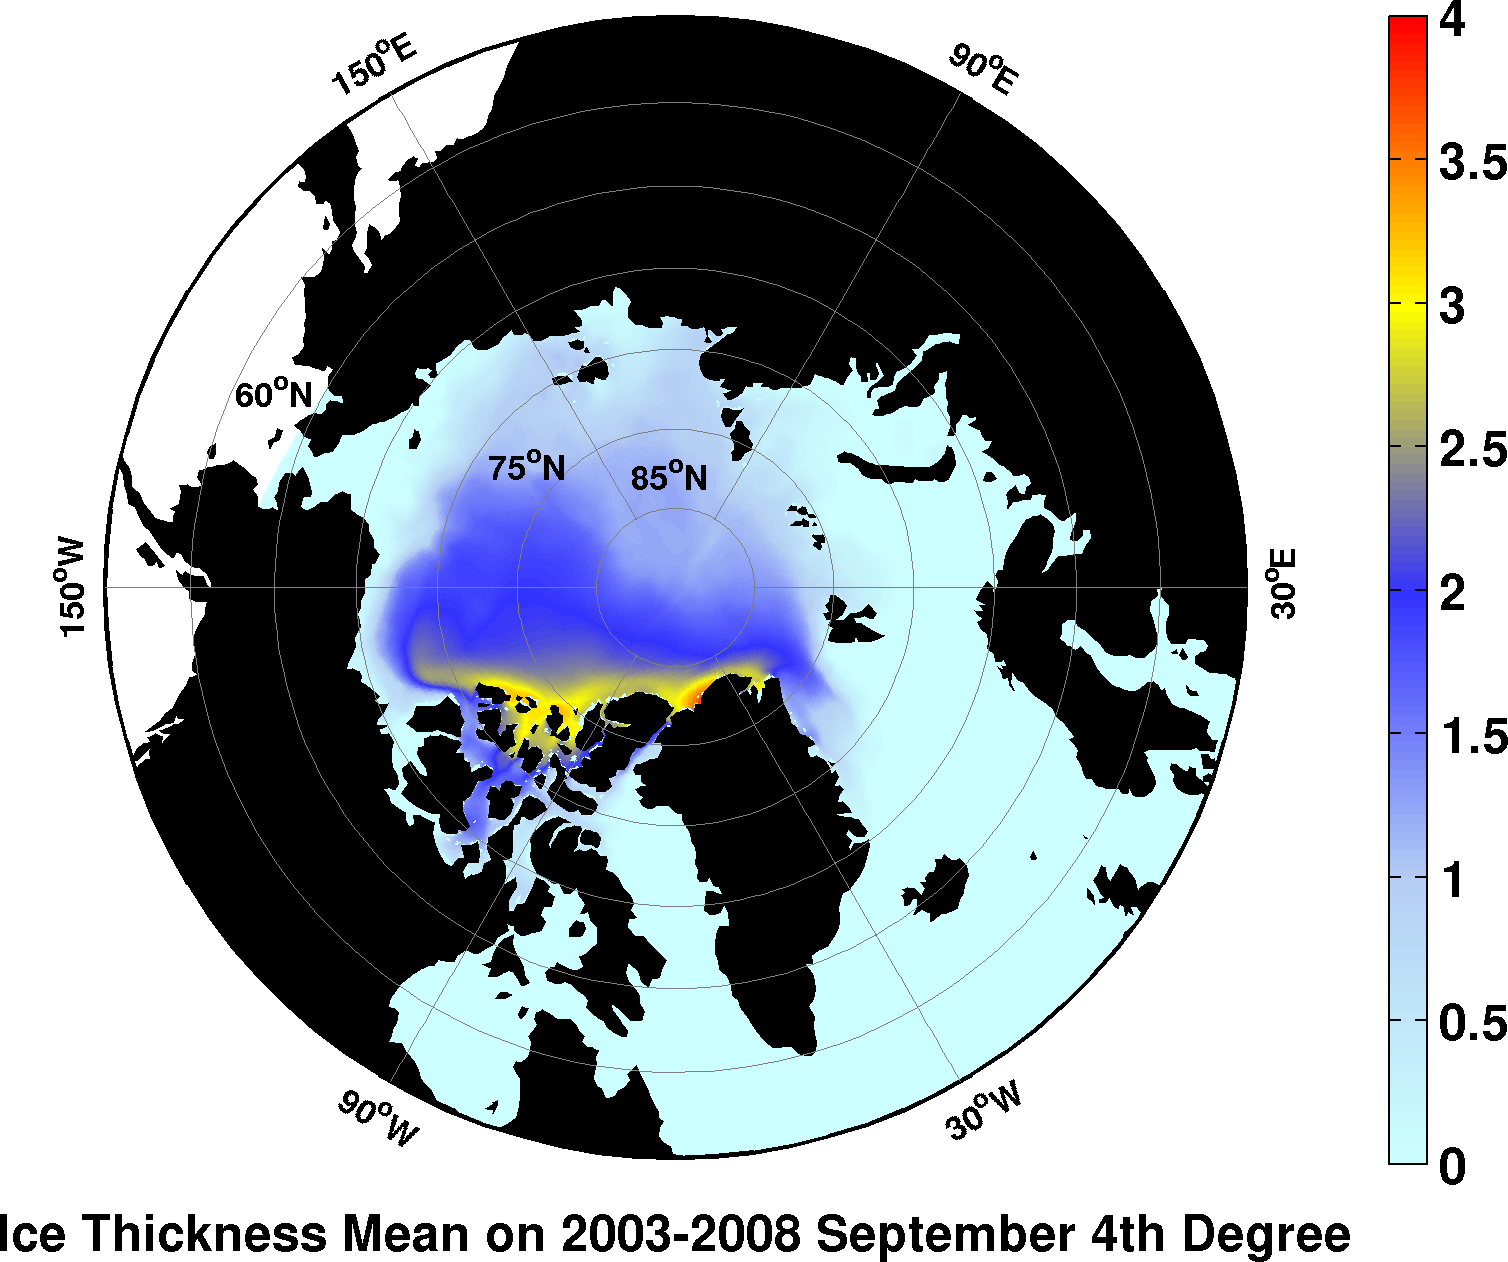
\includegraphics[width=\linewidth]{/home/jingfan/Desktop/Step1/1/Ice_Thickness_mean_2003-2008_September_4th_Degree.png}
\end{column}
\begin{column}[t]{0.5\linewidth}
\centering
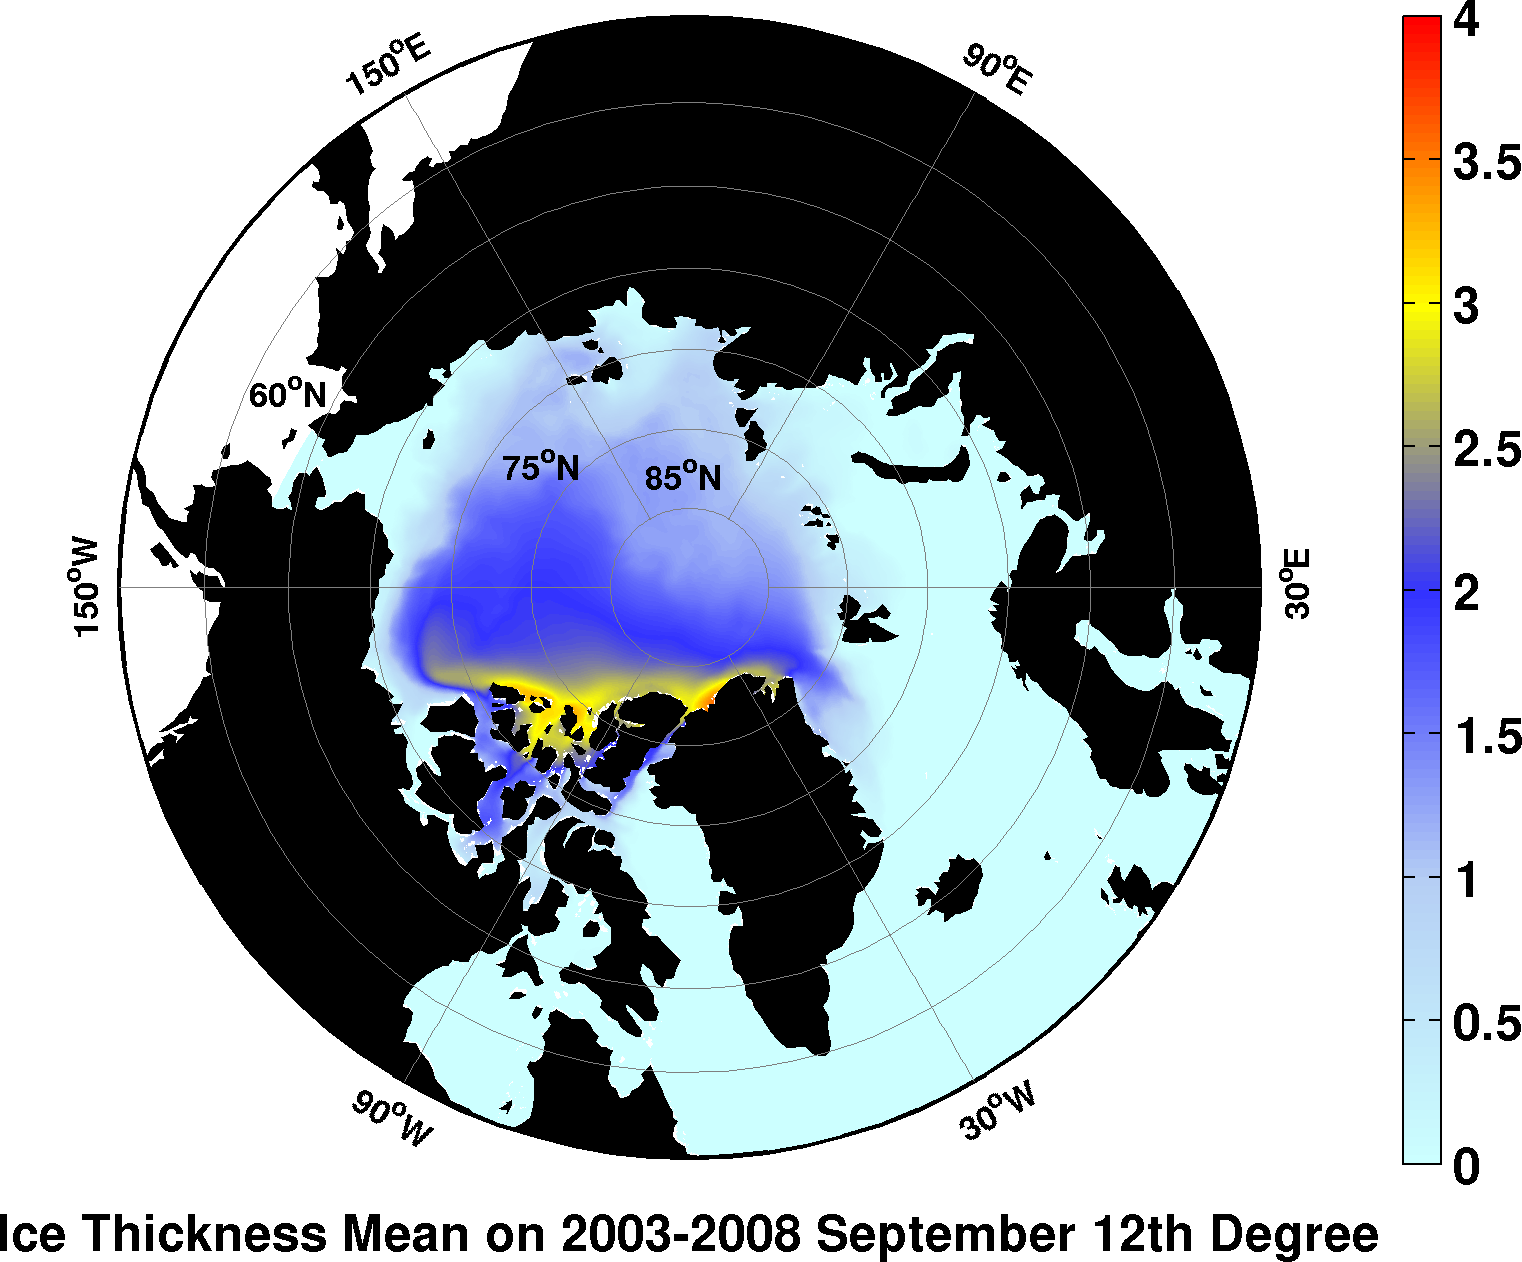
\includegraphics[width=\linewidth]{/home/jingfan/Desktop/Step1/1/Ice_Thickness_mean_2003-2008_September_12th_Degree.png}
\end{column}
\end{columns}

\end{frame}

\begin{frame}
\frametitle{Mean Sea-Ice Thickness Difference(ANHA12-ANHA4)}

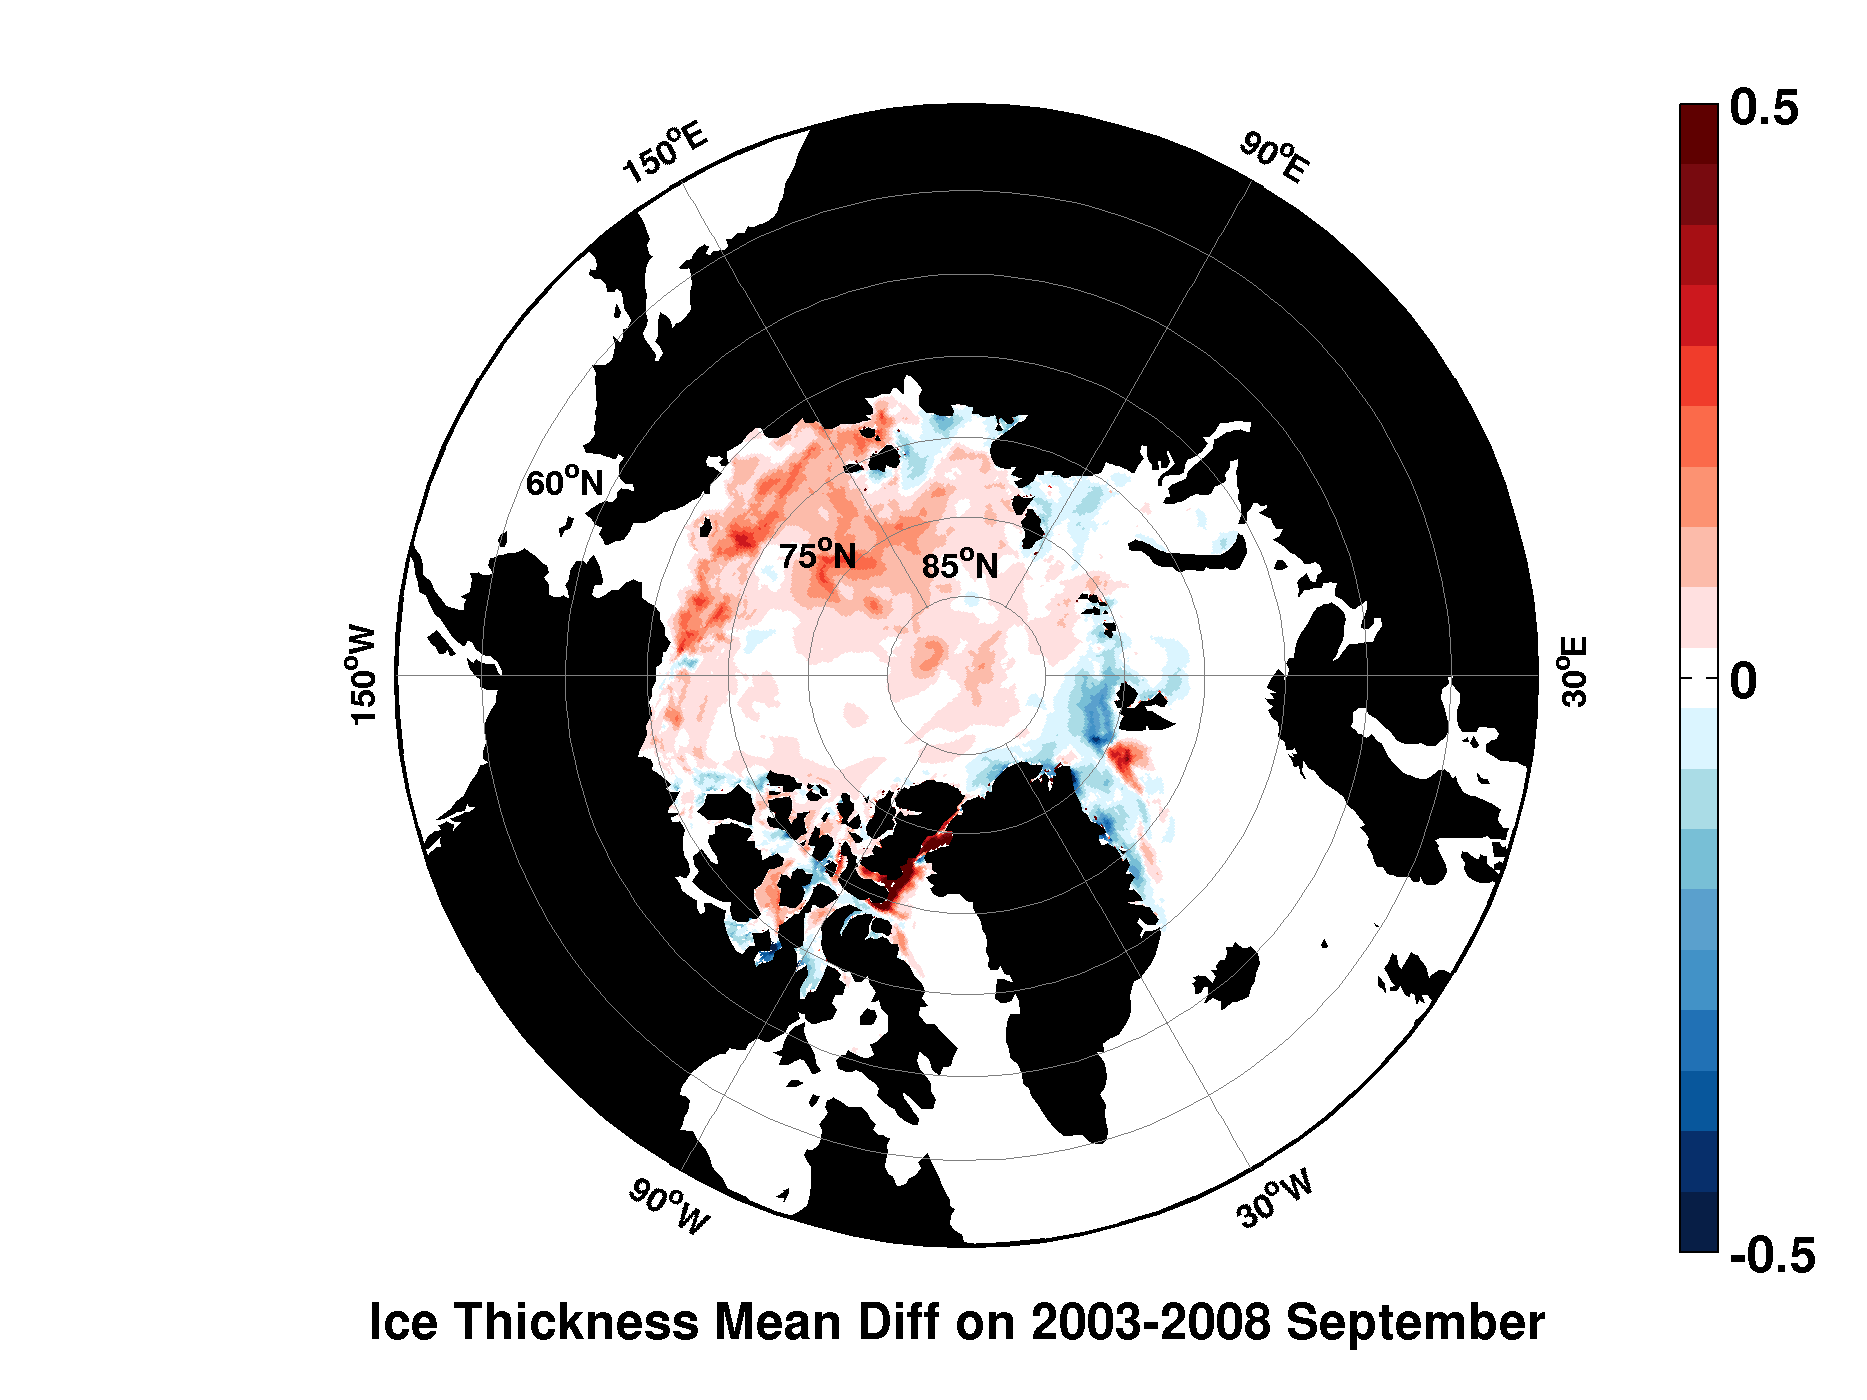
\includegraphics[width=0.9\linewidth]{/home/jingfan/Desktop/Step1/1/Ice_Thickness_mean_Diff_2003-2008_September.png}

\end{frame}

%%%%%%%%%%%%%%%%%%%%%%%%%%%%%%%%%%%%%%%%%%%%%%%%%%%%%%%%%%%%%
\begin{frame}
\frametitle{Sea-Ice Thickness Standard Deviation}
I calculate the standard deviation on each grid point from 2003-2008 with following equation: $$ STD = \sqrt{\frac{1}{N-1}\sum^N_{i=1}(x_i-\mu)^2} $$
The sample for each grid point is a vector of 6 numbers.
\end{frame}

\begin{frame}
\frametitle{Sea-Ice Thickness Standard Deviation}

\begin{columns}
\begin{column}[t]{0.5\linewidth}
\centering
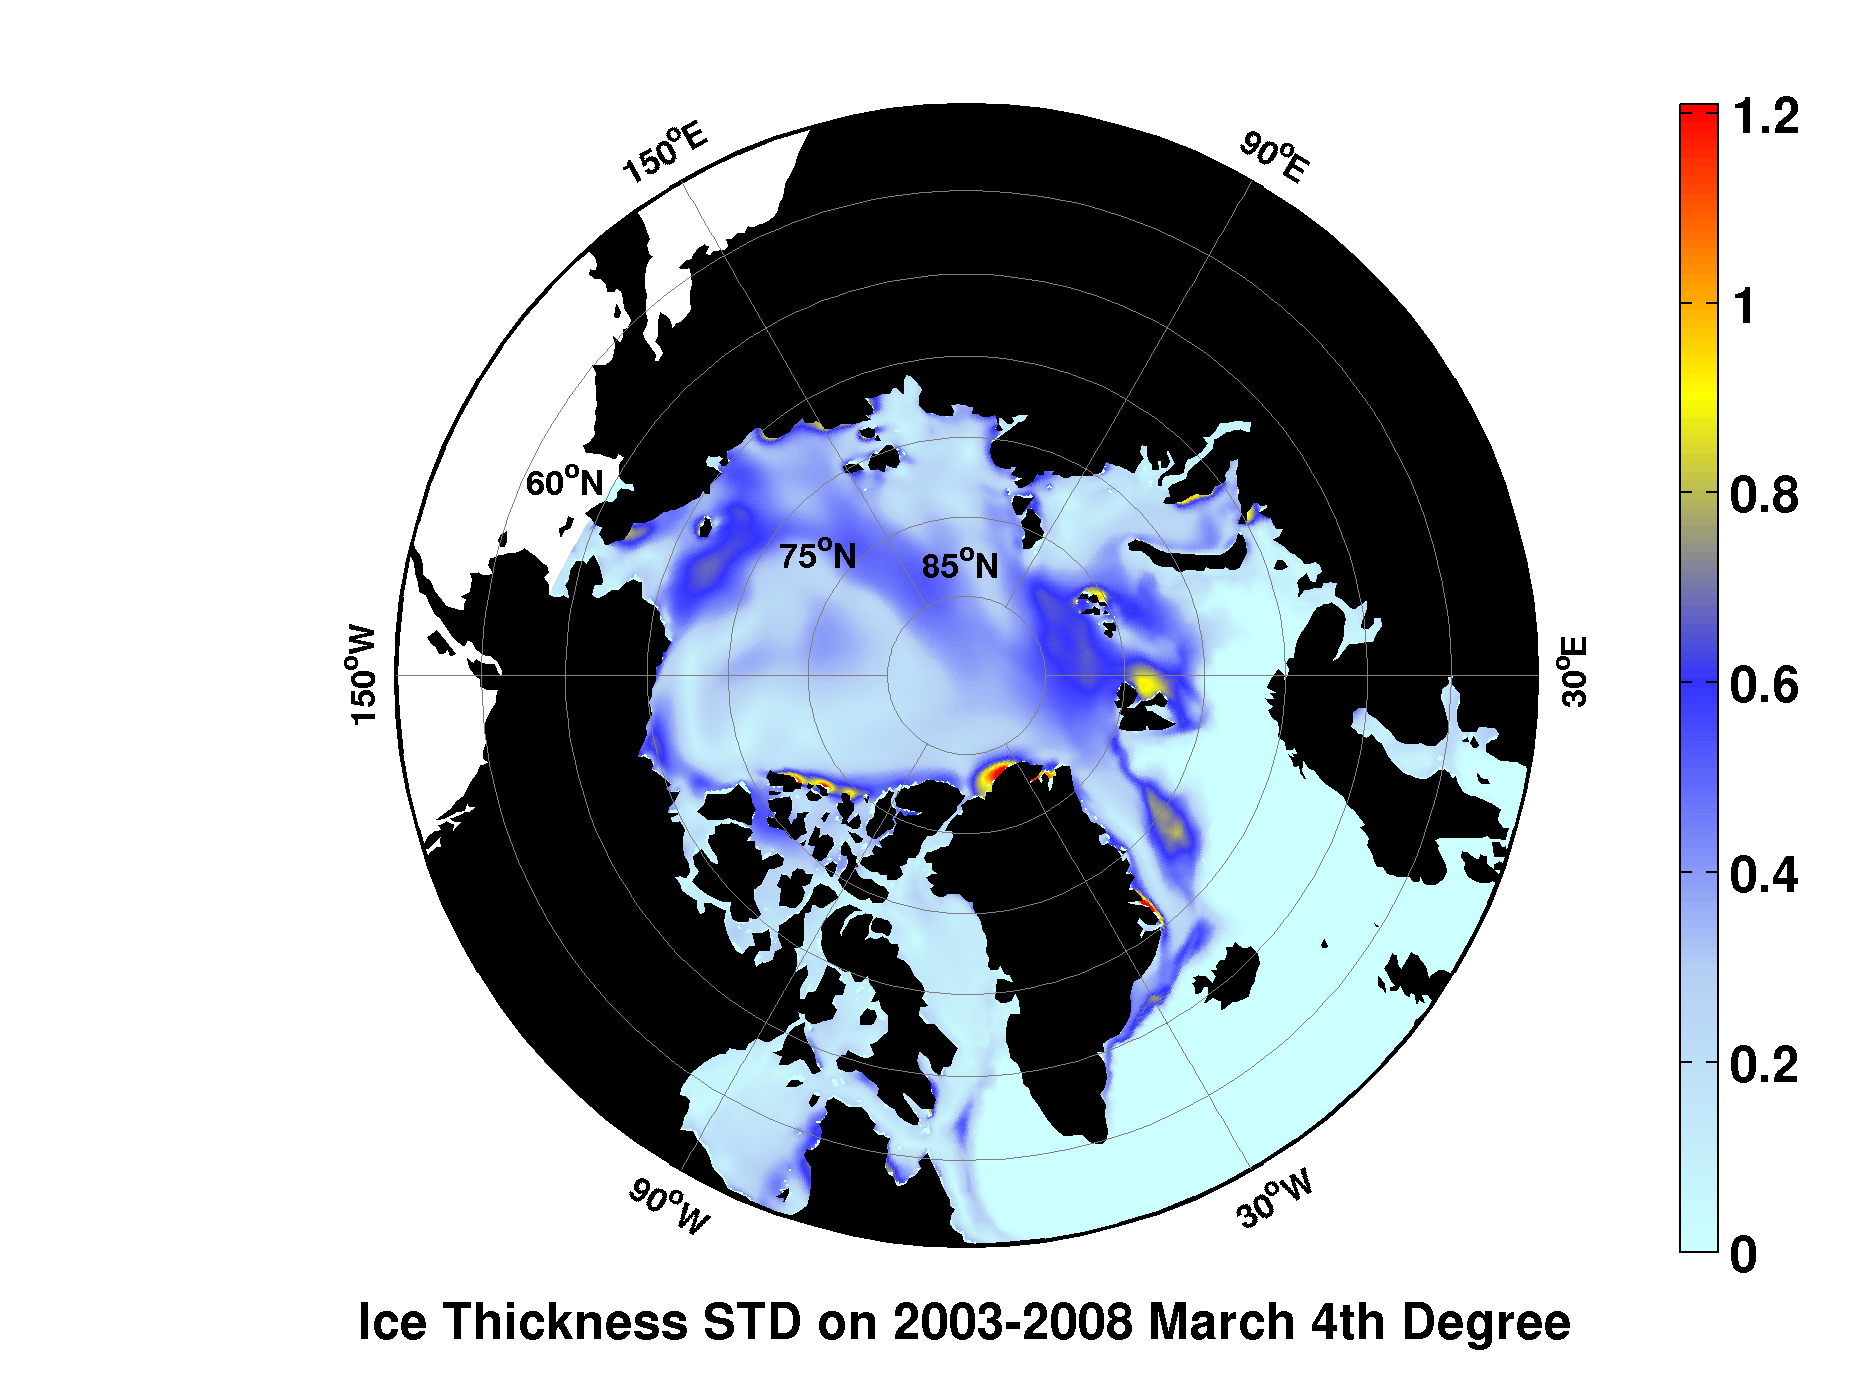
\includegraphics[width=\linewidth]{/home/jingfan/Desktop/Step1/2/Ice_Thickness_STD_2003-2008_March_4th_Degree.png}
\end{column}
\begin{column}[t]{0.5\linewidth}
\centering
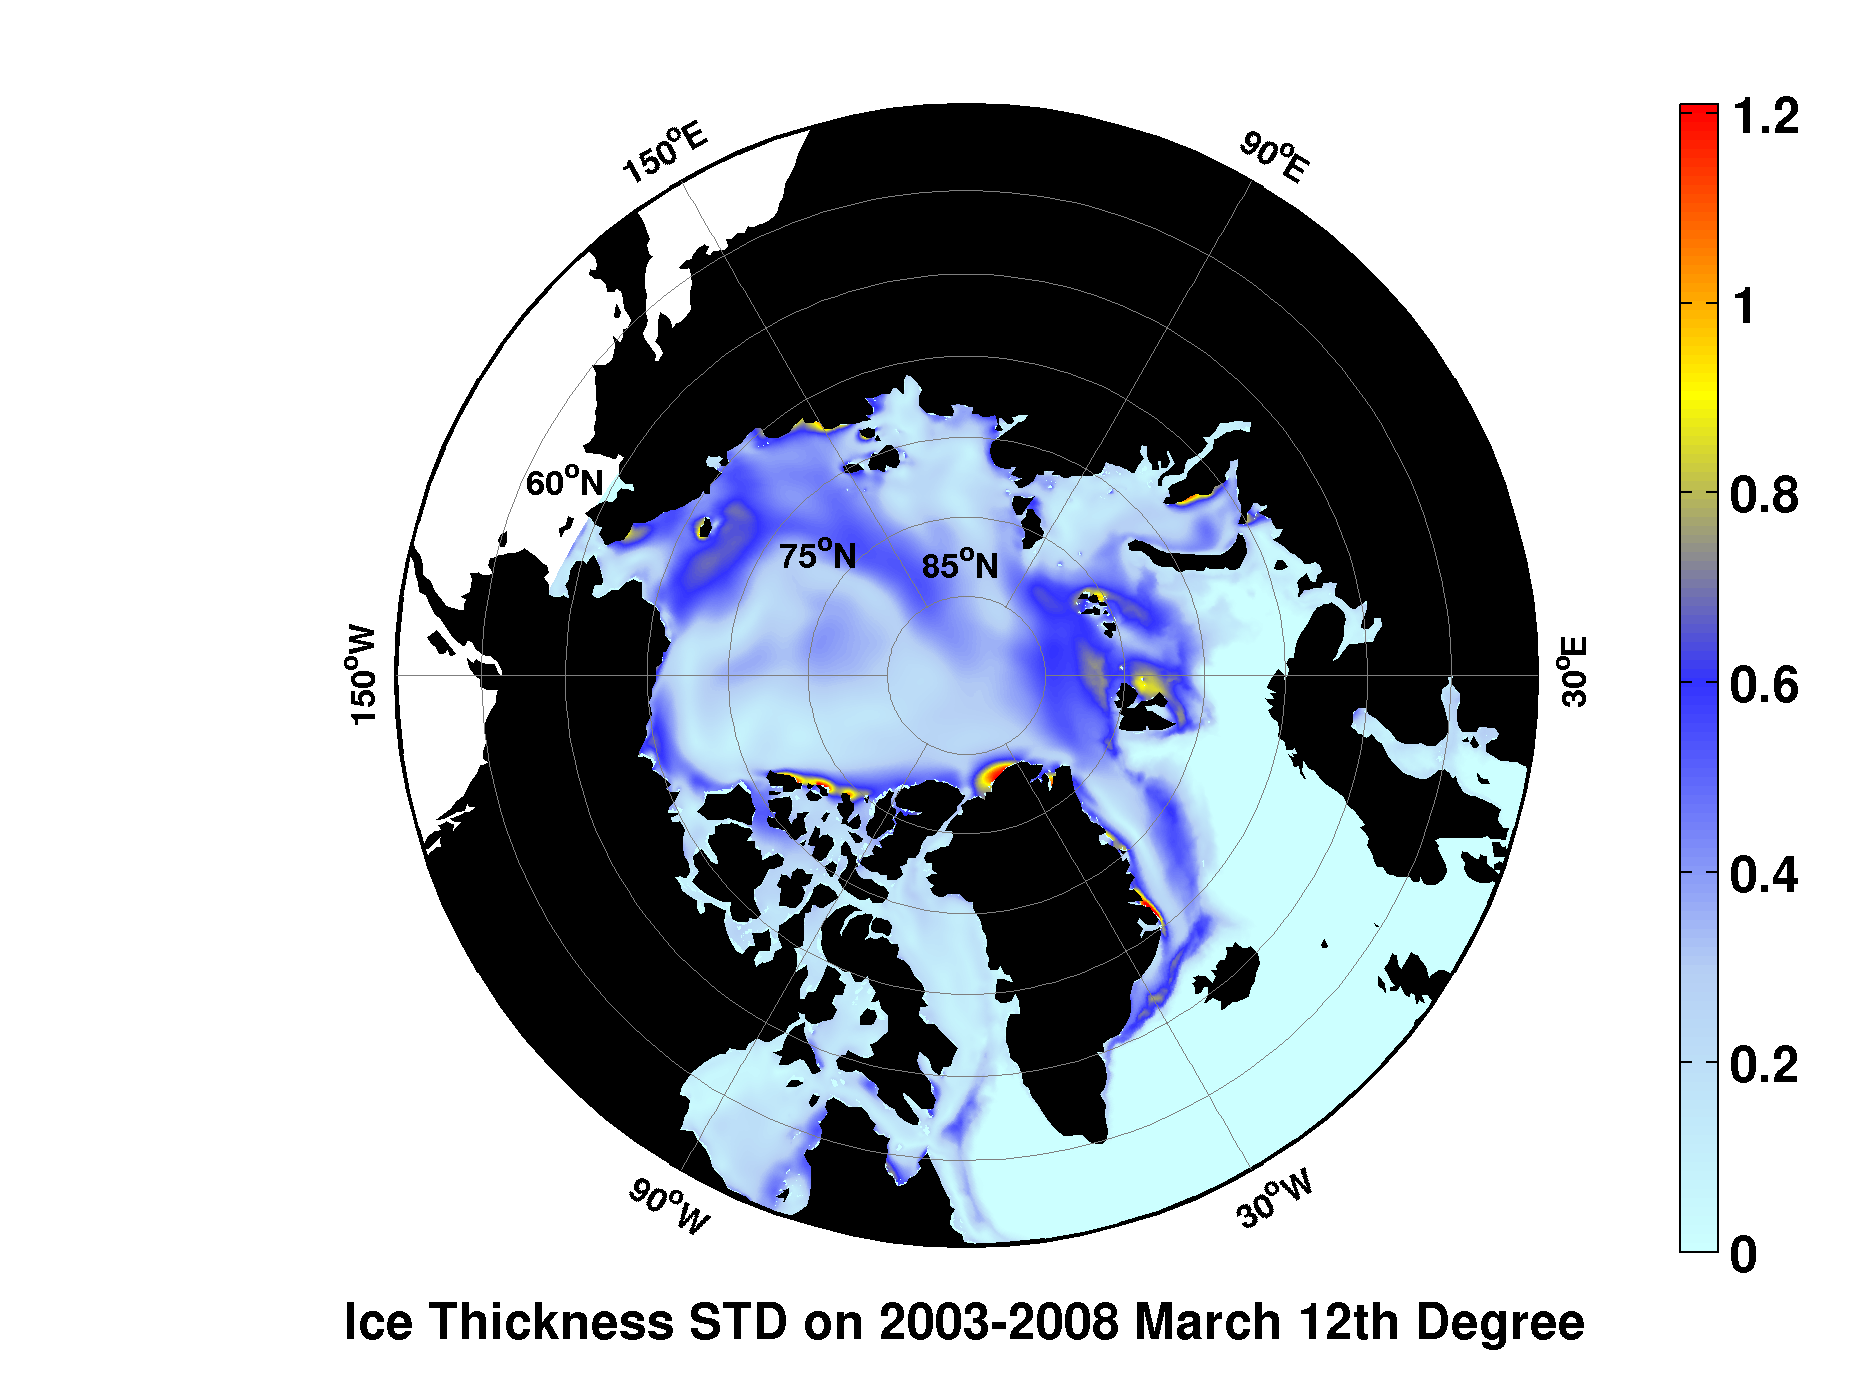
\includegraphics[width=\linewidth]{/home/jingfan/Desktop/Step1/2/Ice_Thickness_STD_2003-2008_March_12th_Degree.png}
\end{column}
\end{columns}

\end{frame}

\begin{frame}
\frametitle{Sea-Ice Thickness Standard Deviation Difference(ANHA12-ANHA4)}

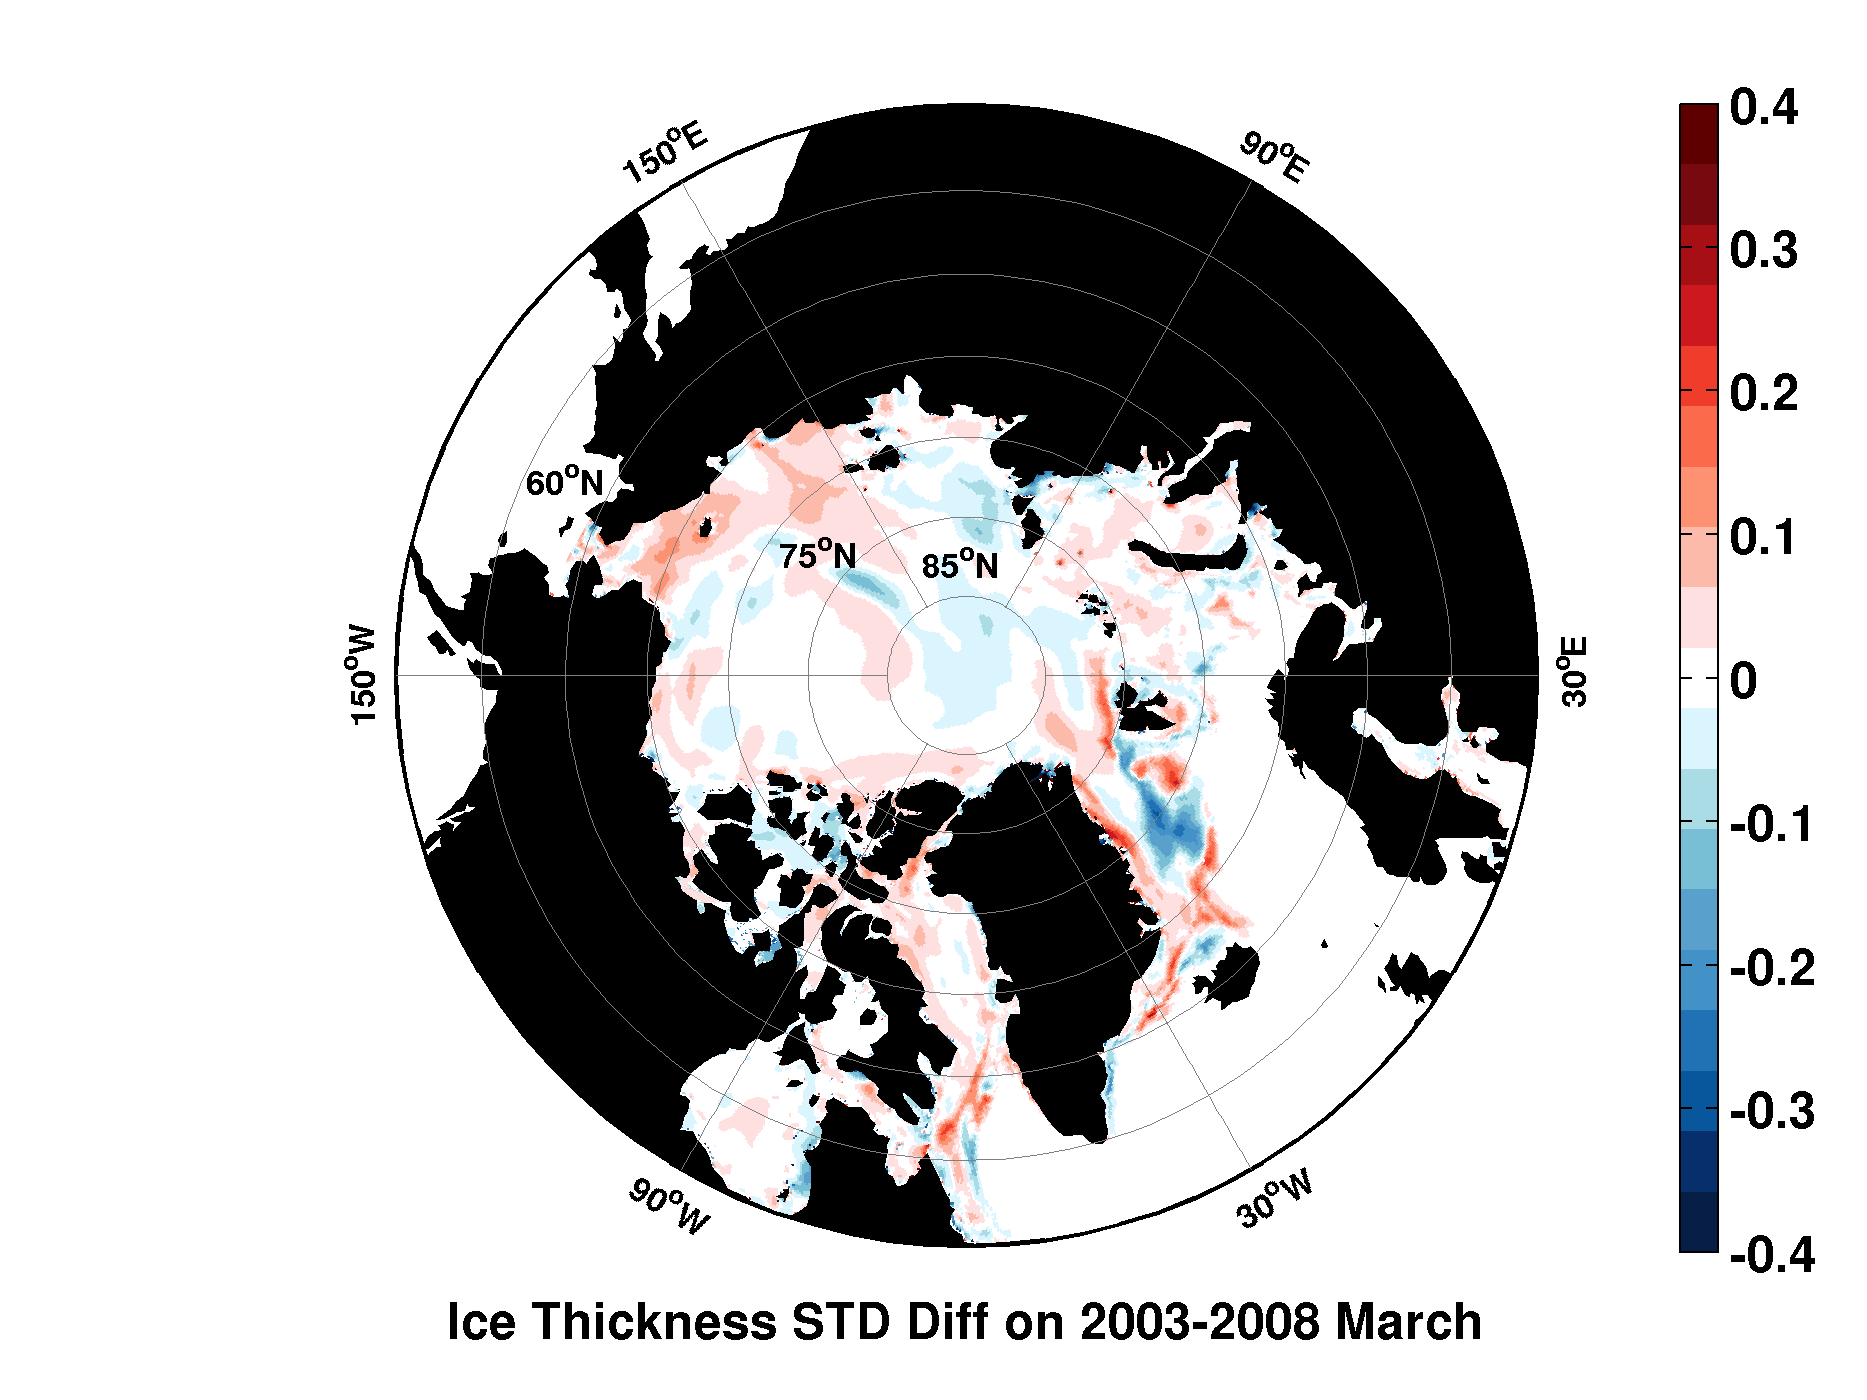
\includegraphics[width=0.9\linewidth]{/home/jingfan/Desktop/Step1/2/Ice_Thickness_STD_Diff_2003-2008_March.png}

\end{frame}

\begin{frame}
\frametitle{Sea-Ice Thickness Standard Deviation}

\begin{columns}
\begin{column}[t]{0.5\linewidth}
\centering
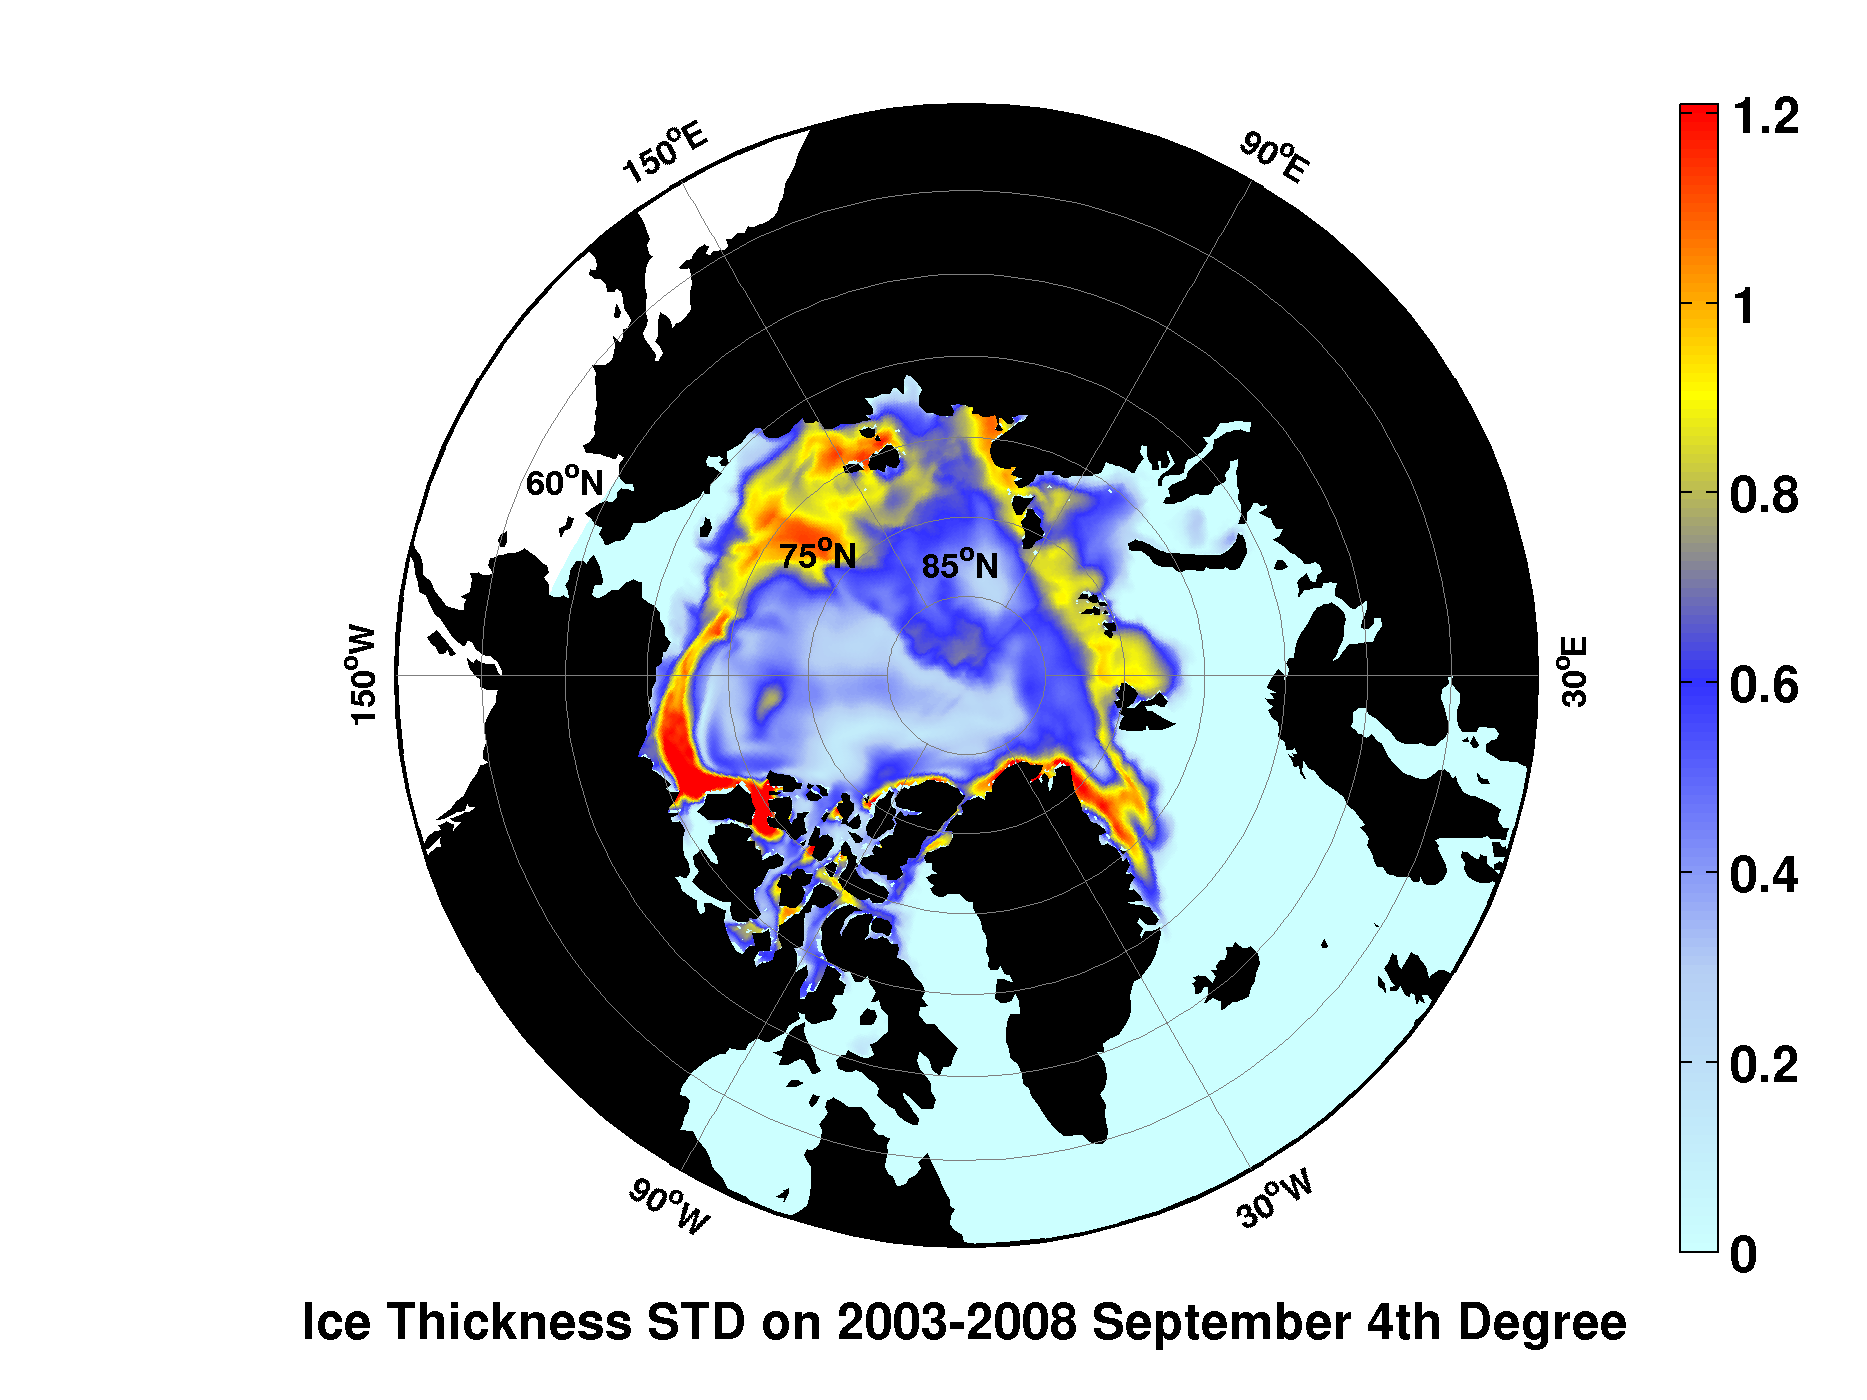
\includegraphics[width=\linewidth]{/home/jingfan/Desktop/Step1/2/Ice_Thickness_STD_2003-2008_September_4th_Degree.png}
\end{column}
\begin{column}[t]{0.5\linewidth}
\centering
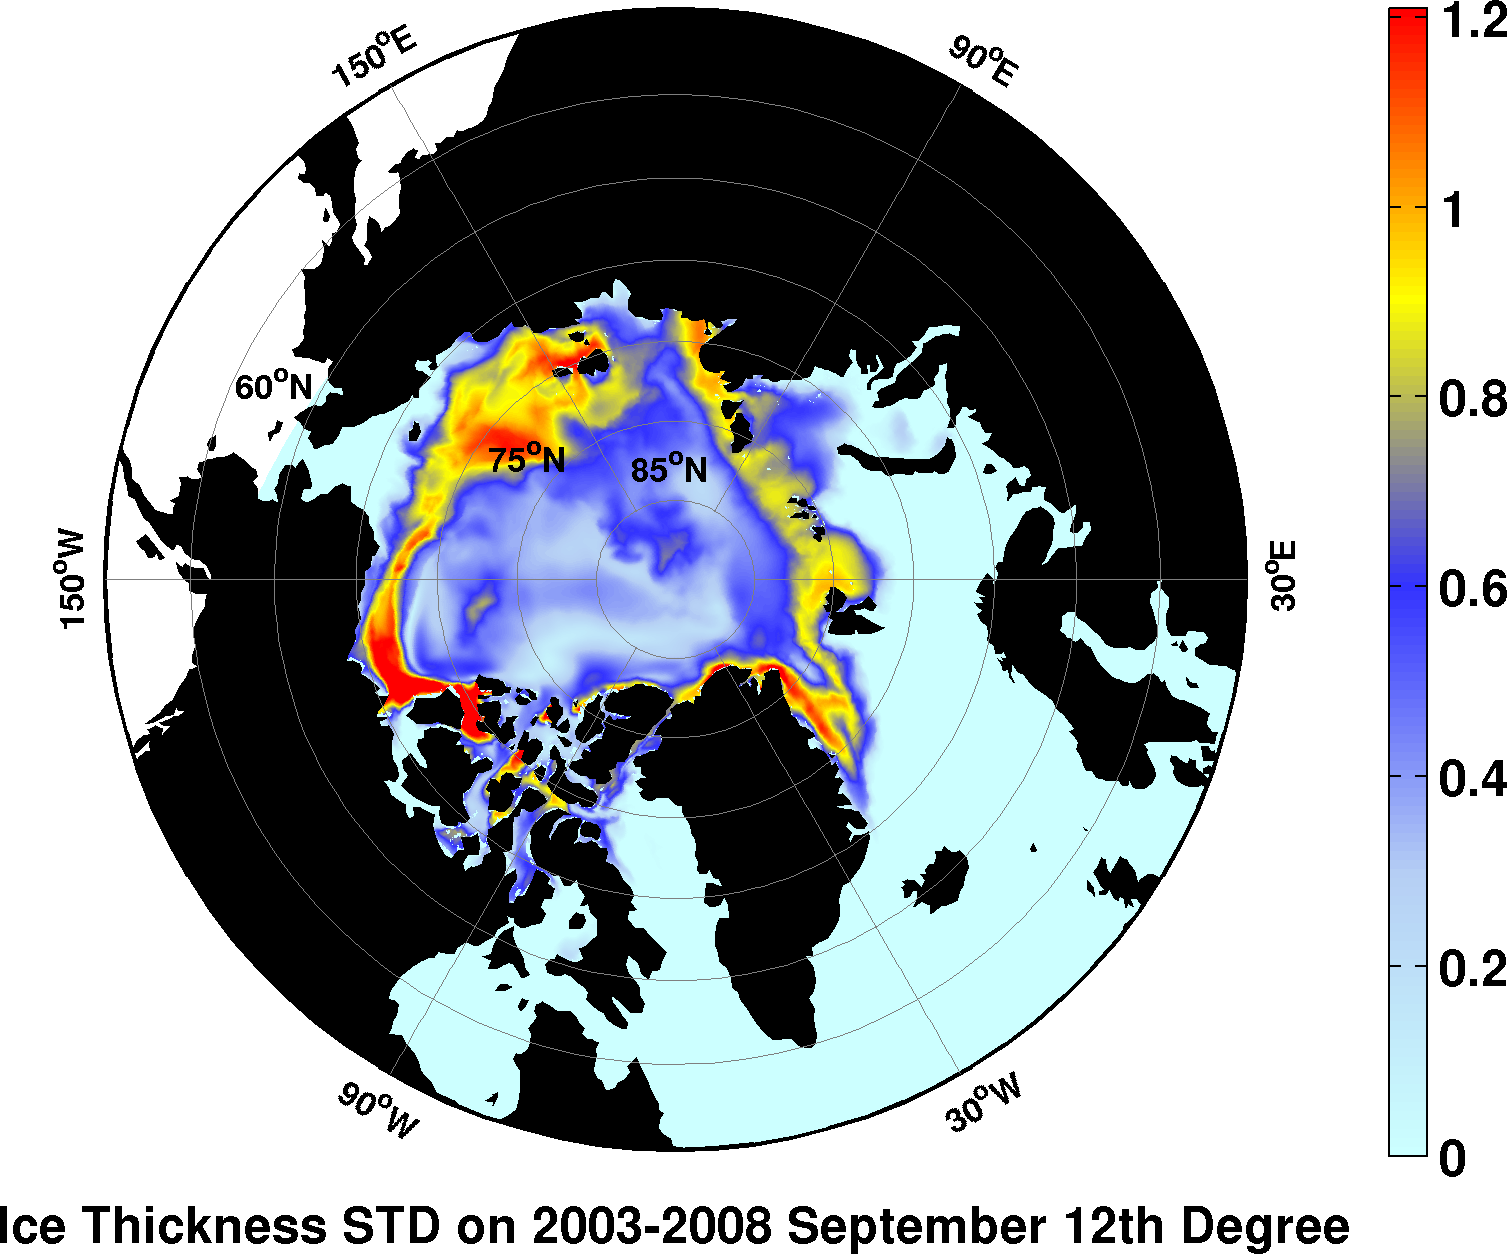
\includegraphics[width=\linewidth]{/home/jingfan/Desktop/Step1/2/Ice_Thickness_STD_2003-2008_September_12th_Degree.png}
\end{column}
\end{columns}

\end{frame}

\begin{frame}
\frametitle{Sea-Ice Thickness Standard Deviation Difference(ANHA12-ANHA4)}

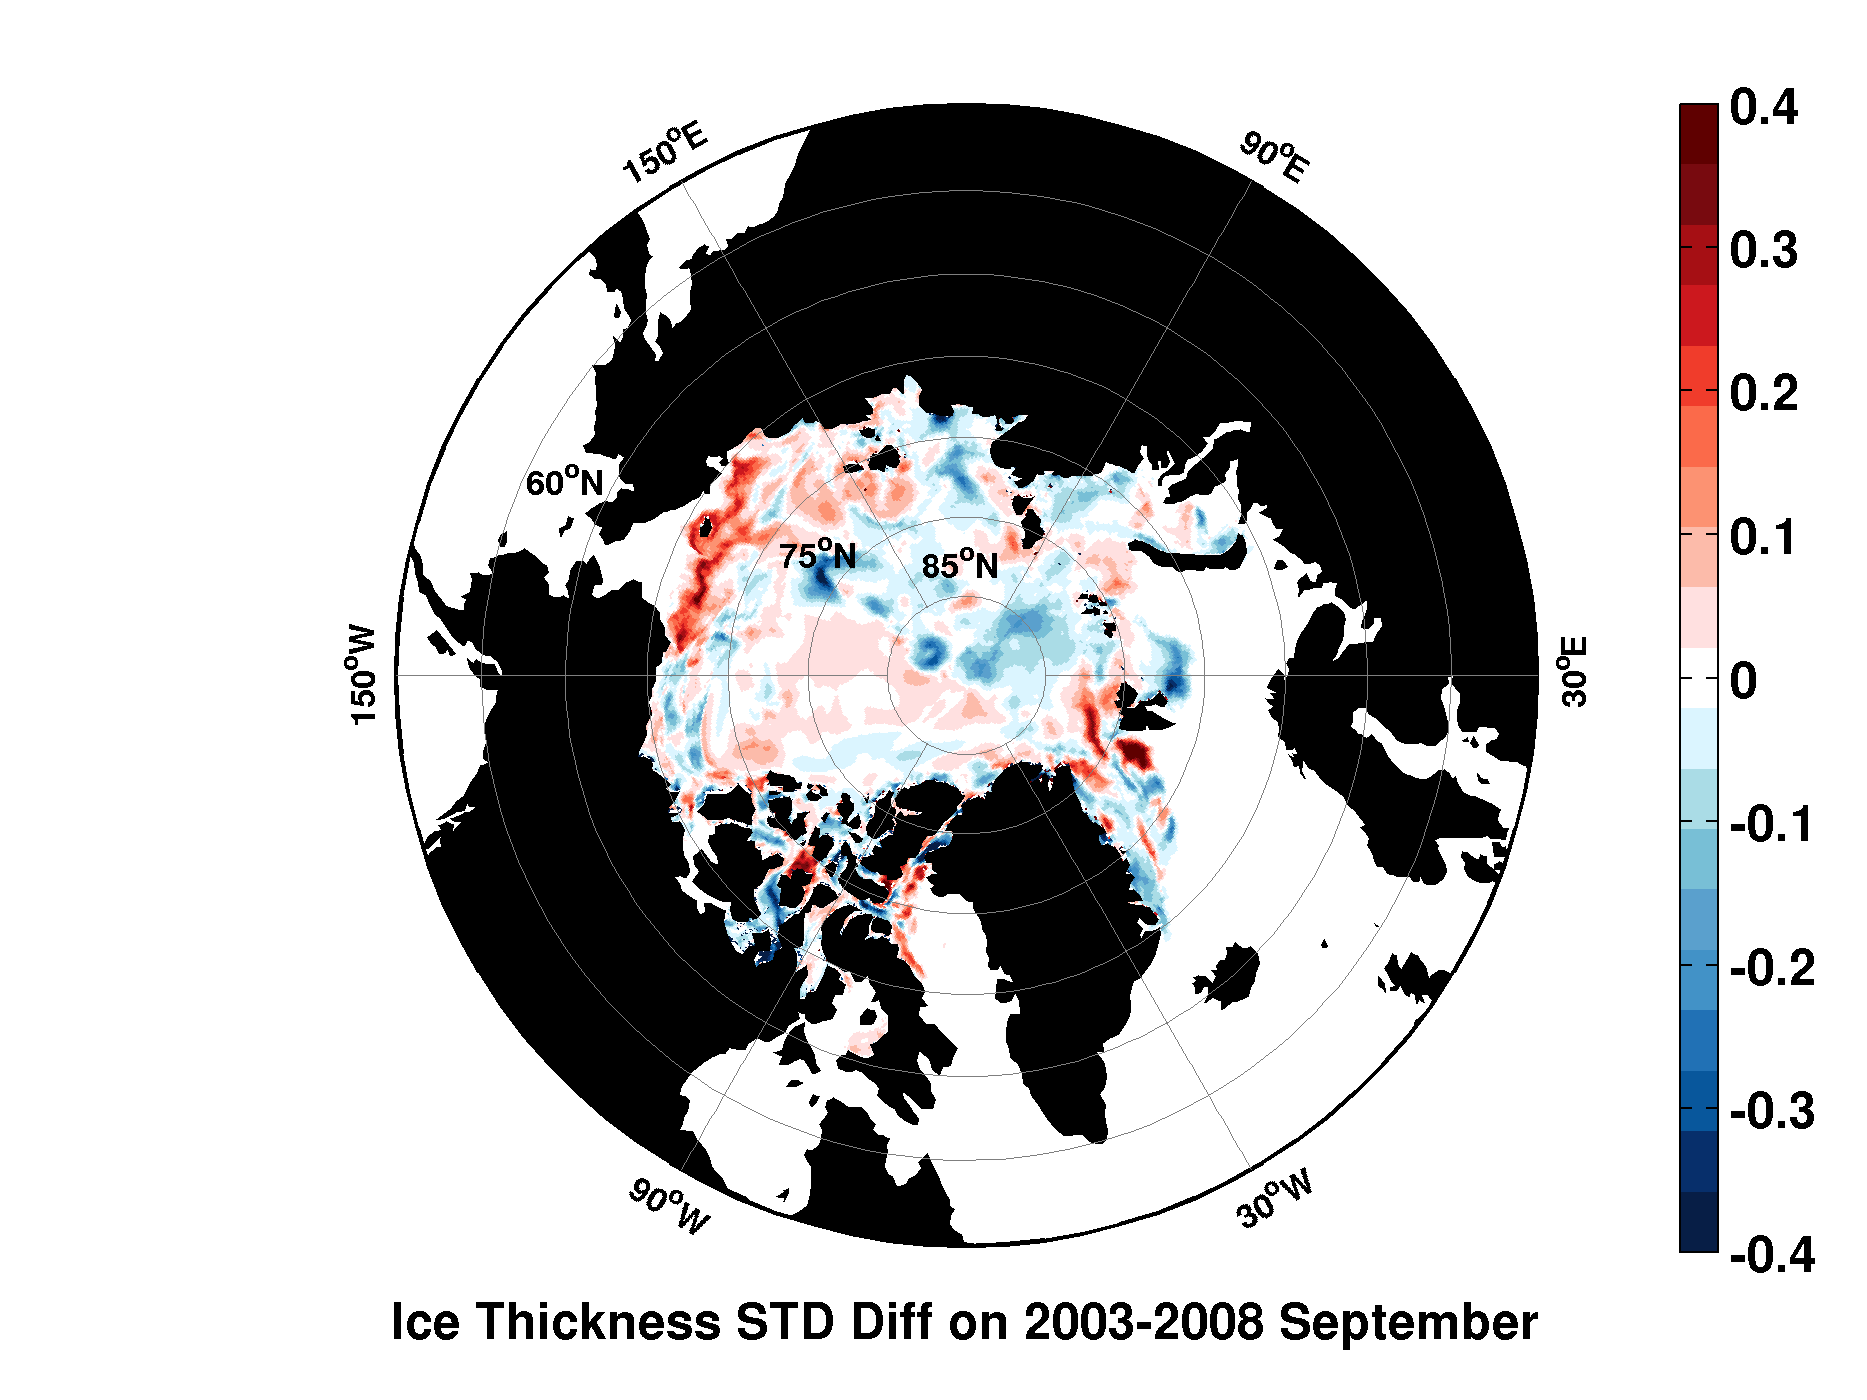
\includegraphics[width=0.9\linewidth]{/home/jingfan/Desktop/Step1/2/Ice_Thickness_STD_Diff_2003-2008_September.png}

\end{frame}

%%%%%%%%%%%%%%%%%%%%%%%%%%%%%%%%%%%%%%%%%%%%%%%%%%%%%%%%%%%%%
\begin{frame}
\frametitle{Sea-Ice Thickness September 2007}
Simply plot Sea-Ice Thickness on each day in September 2007 along with difference plots of different configuration.
\end{frame}

\begin{frame}
\frametitle{Sea-Ice Thickness September 2007}

\begin{columns}
\begin{column}[t]{0.5\linewidth}
\centering
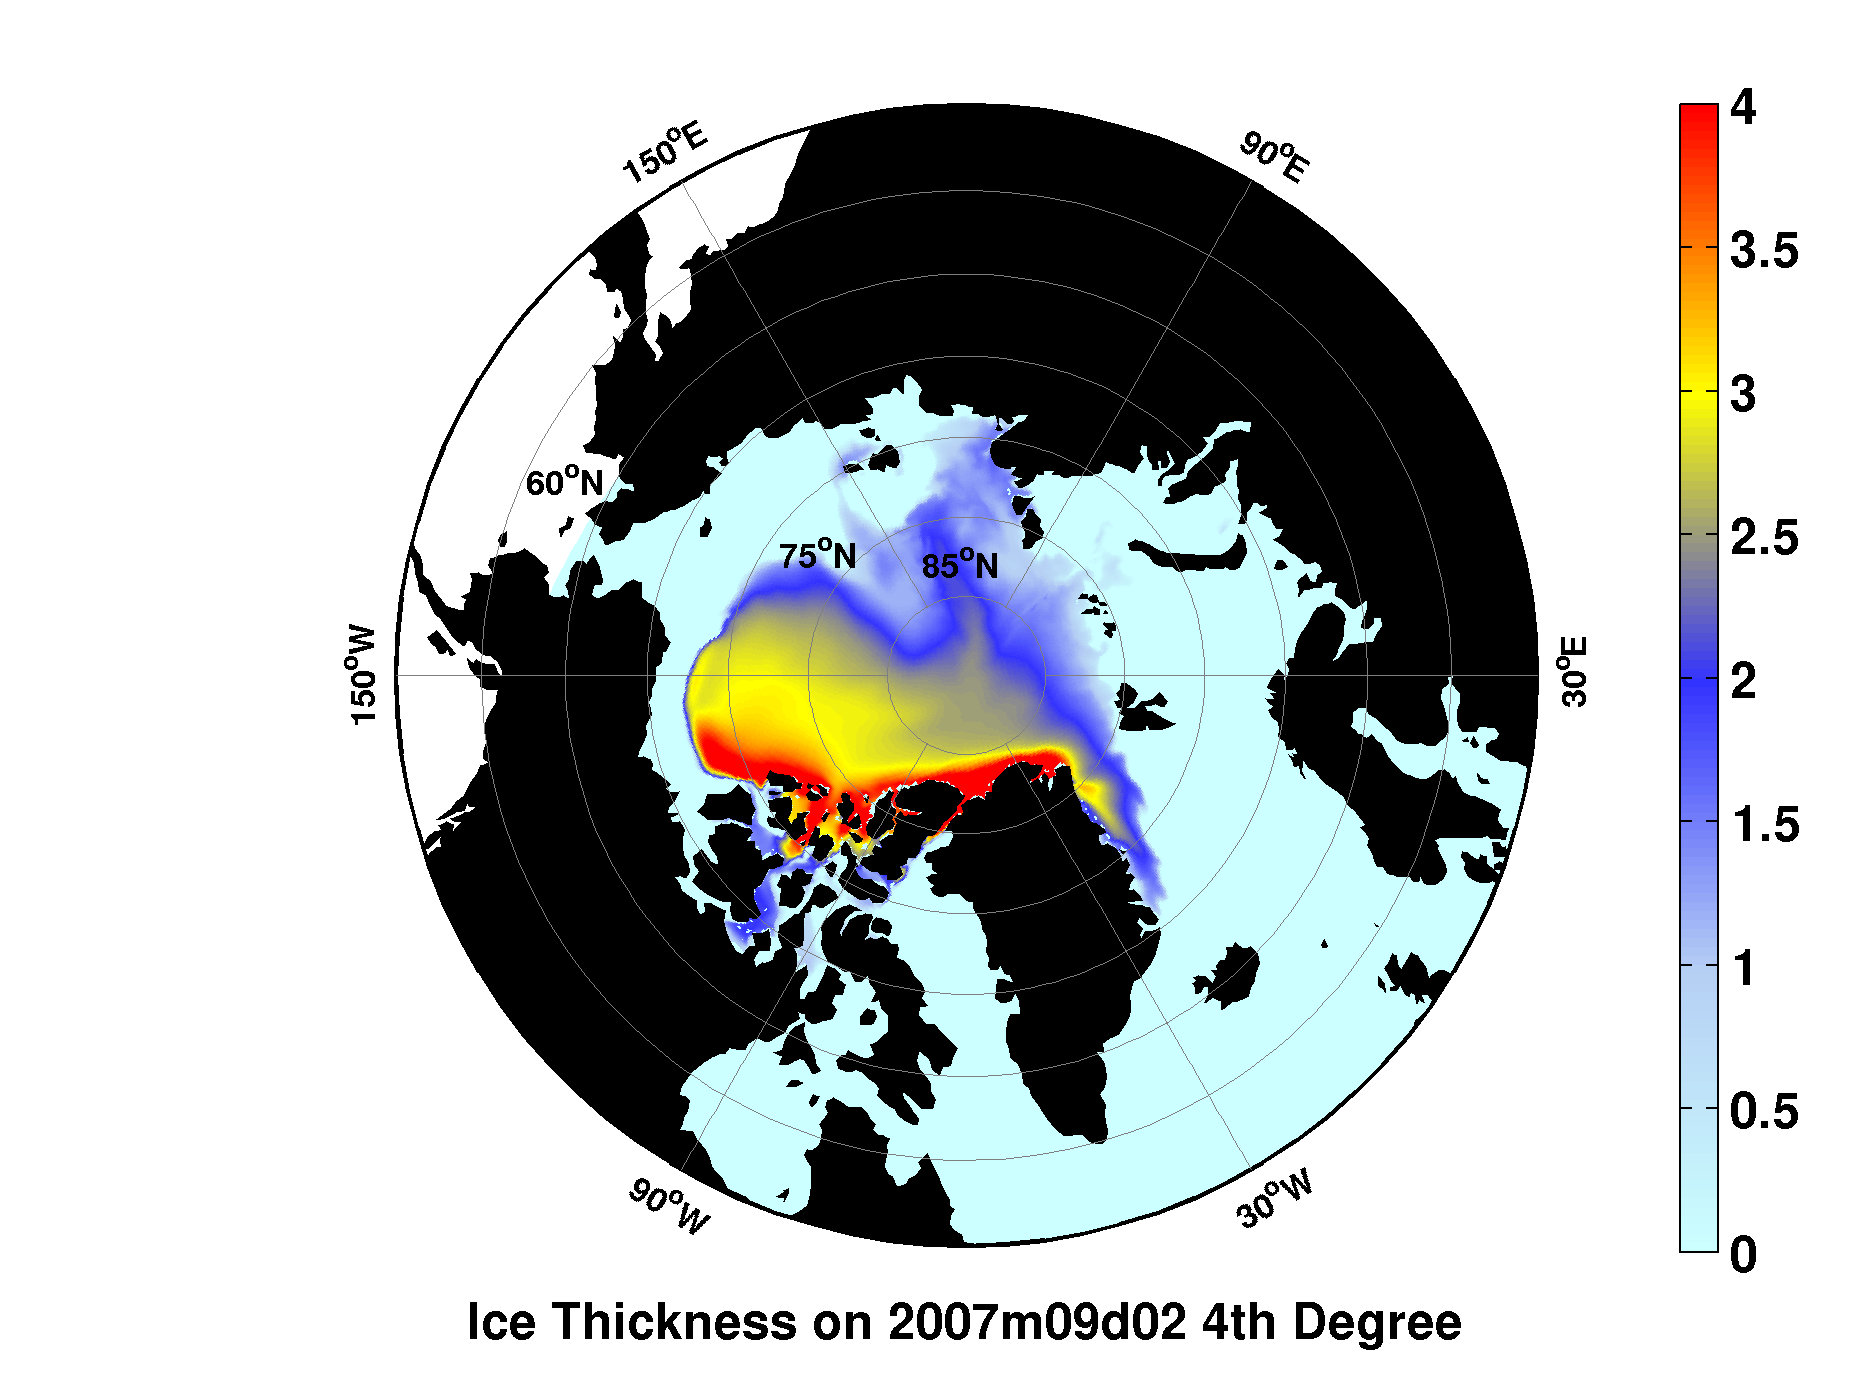
\includegraphics[width=\linewidth]{/home/jingfan/Desktop/Step1/3/Ice_Thickness_2007m09d02_4th_Degree.png}
\end{column}
\begin{column}[t]{0.5\linewidth}
\centering
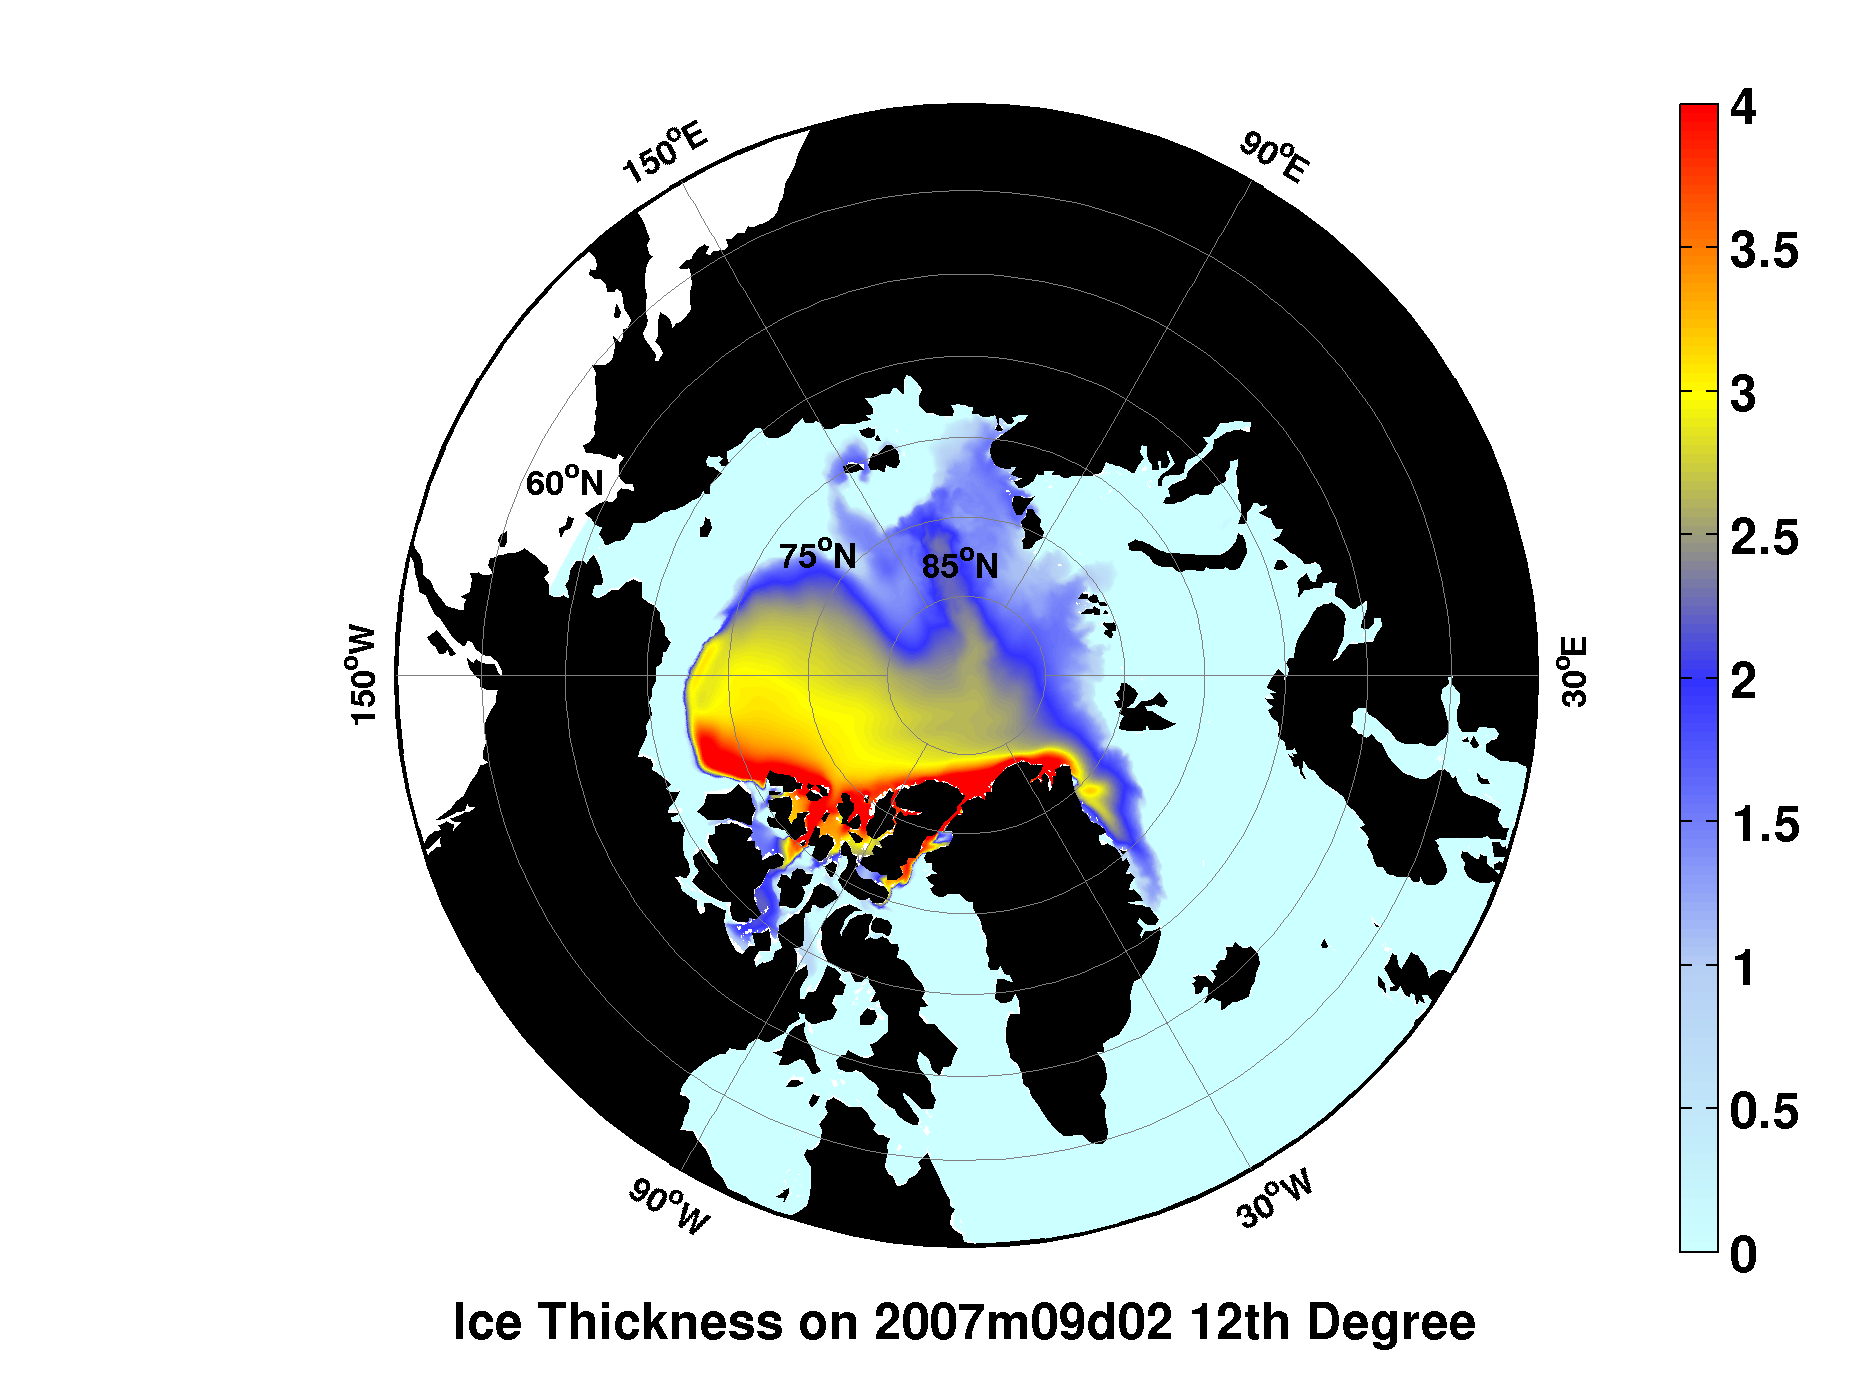
\includegraphics[width=\linewidth]{/home/jingfan/Desktop/Step1/3/Ice_Thickness_2007m09d02_12th_Degree.png}
\end{column}
\end{columns}

\end{frame}

\begin{frame}
\frametitle{Sea-Ice Thickness September 2007 Difference(ANHA12-ANHA4)}

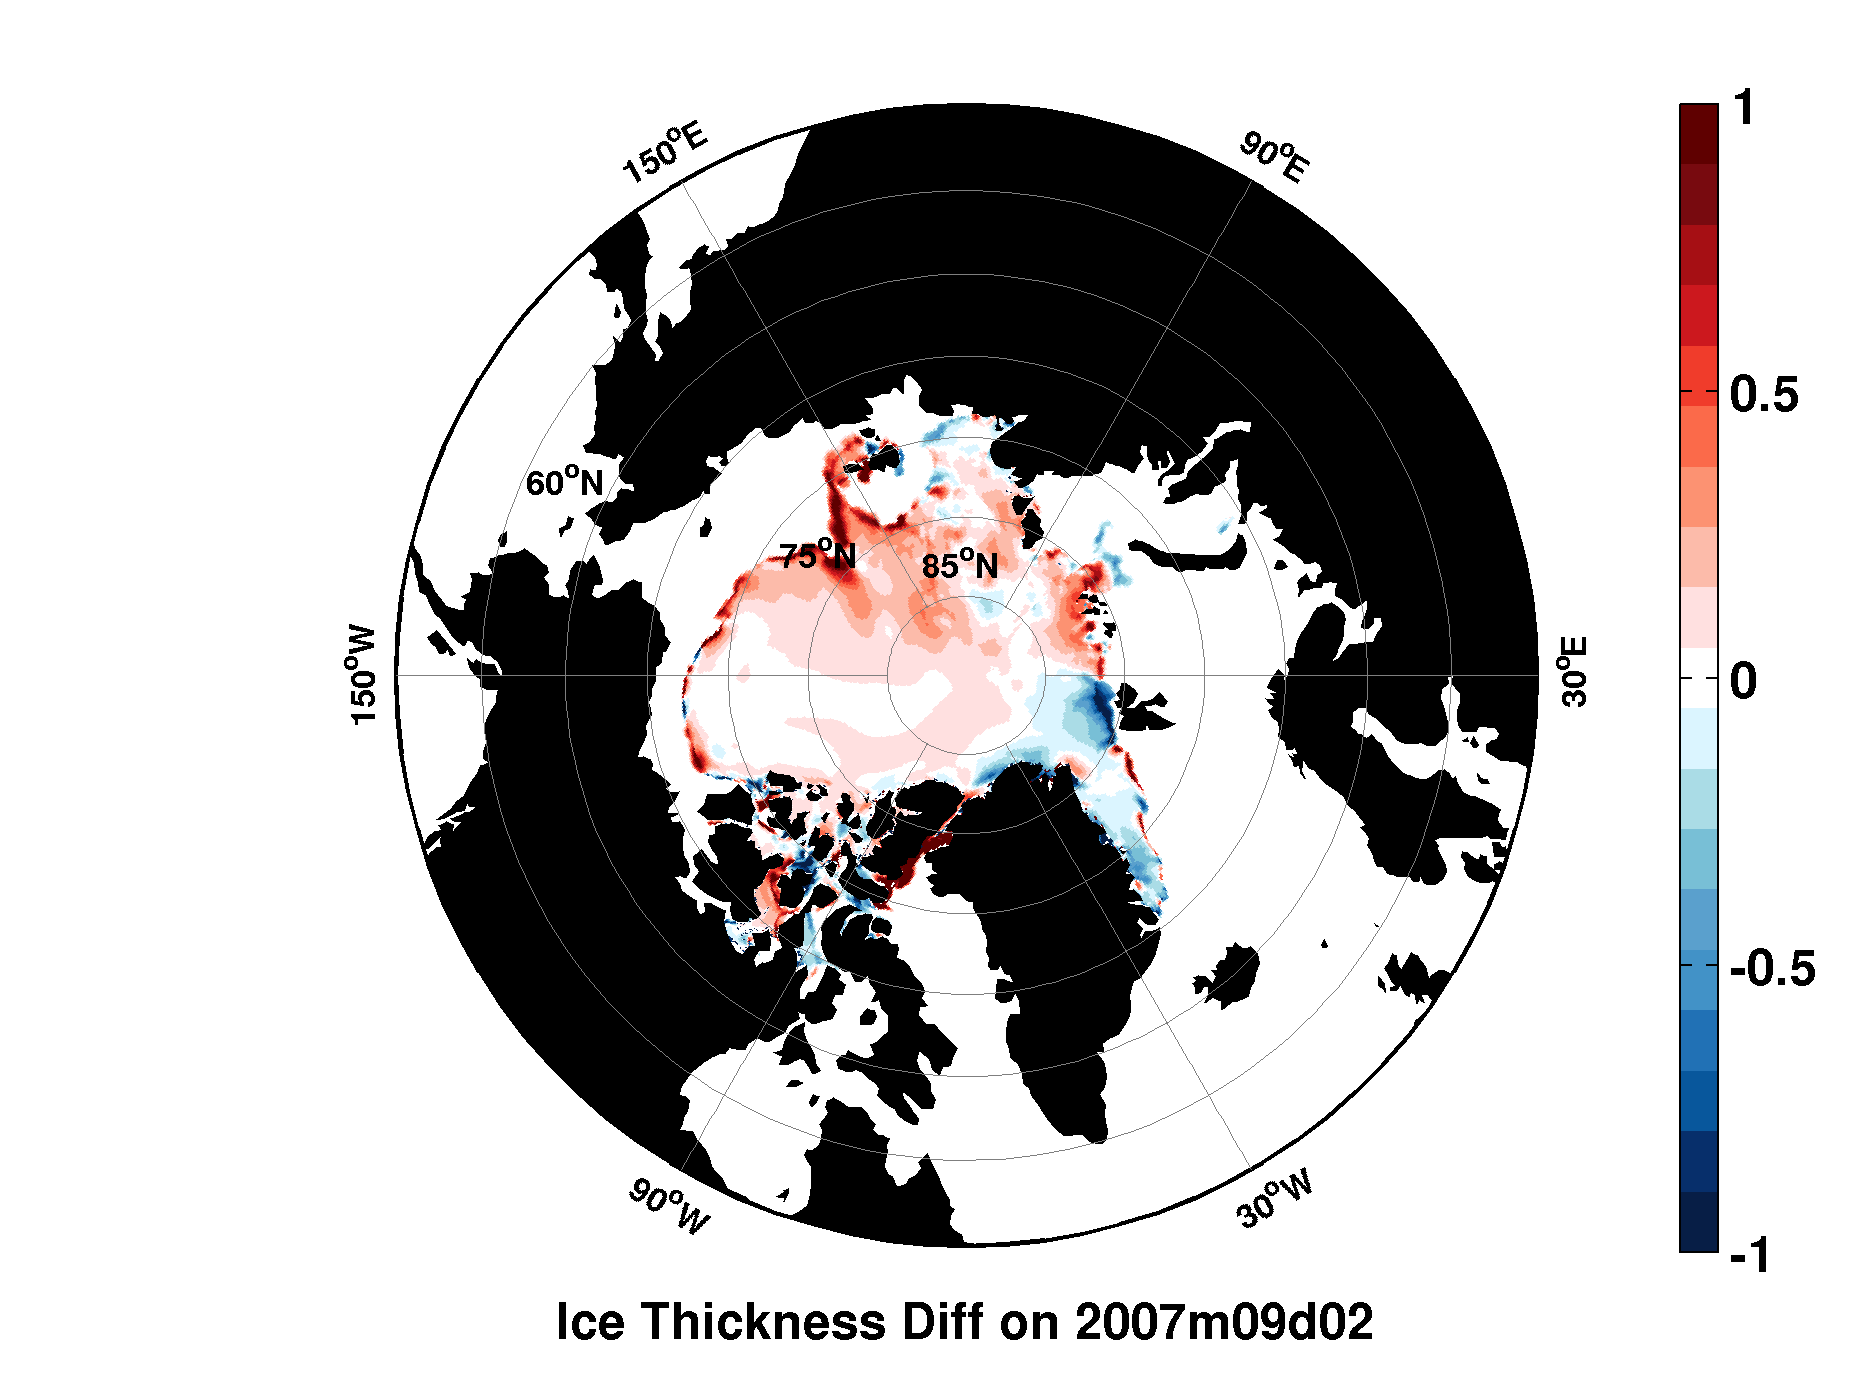
\includegraphics[width=0.9\linewidth]{/home/jingfan/Desktop/Step1/3/Ice_Thickness_Diff_2007m09d02.png}

\end{frame}

\begin{frame}
\frametitle{Sea-Ice Thickness September 2007}

\begin{columns}
\begin{column}[t]{0.5\linewidth}
\centering
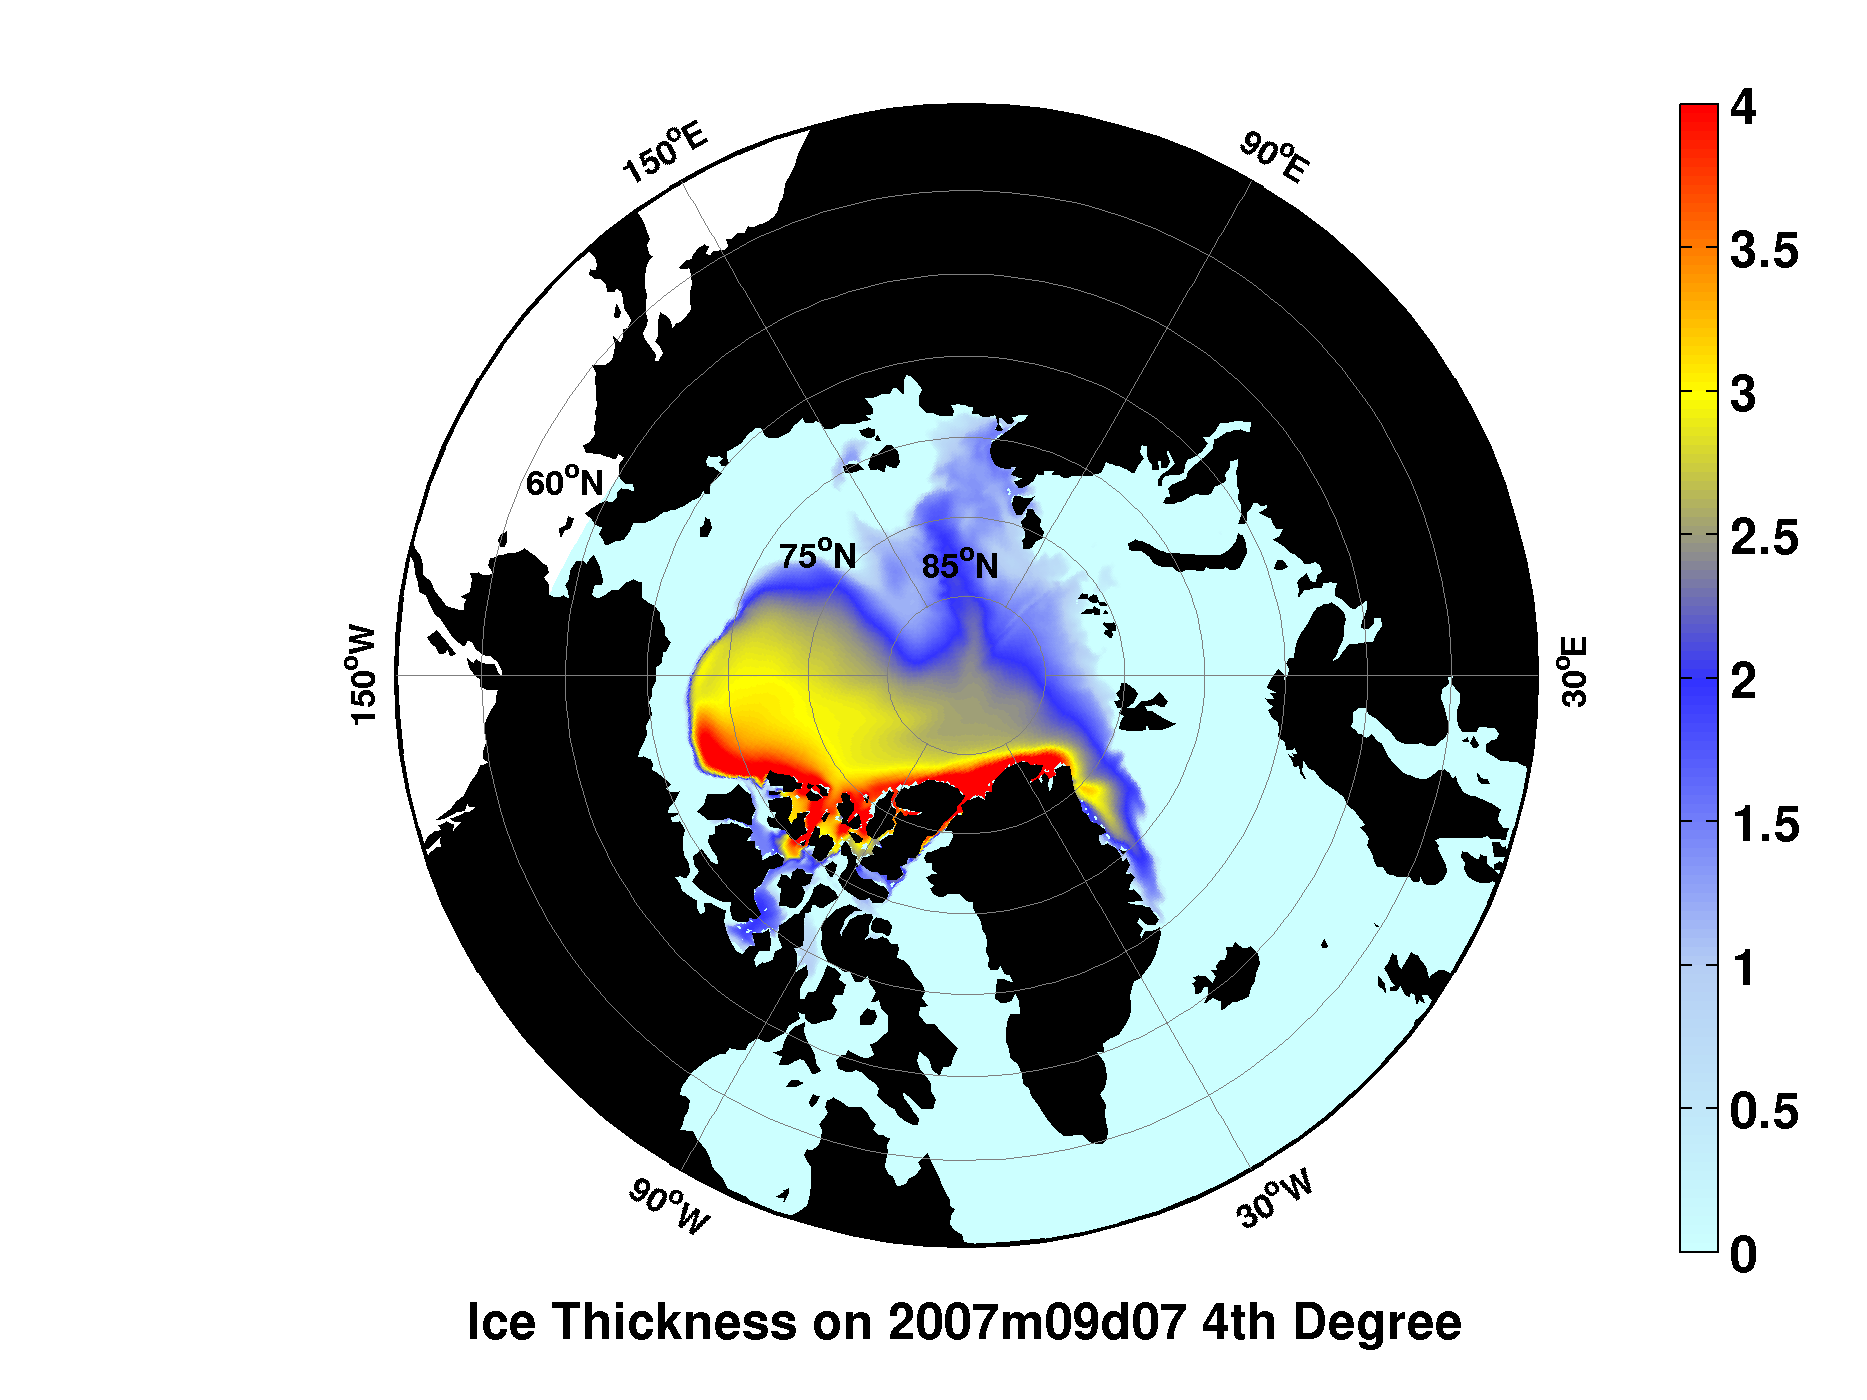
\includegraphics[width=\linewidth]{/home/jingfan/Desktop/Step1/3/Ice_Thickness_2007m09d07_4th_Degree.png}
\end{column}
\begin{column}[t]{0.5\linewidth}
\centering
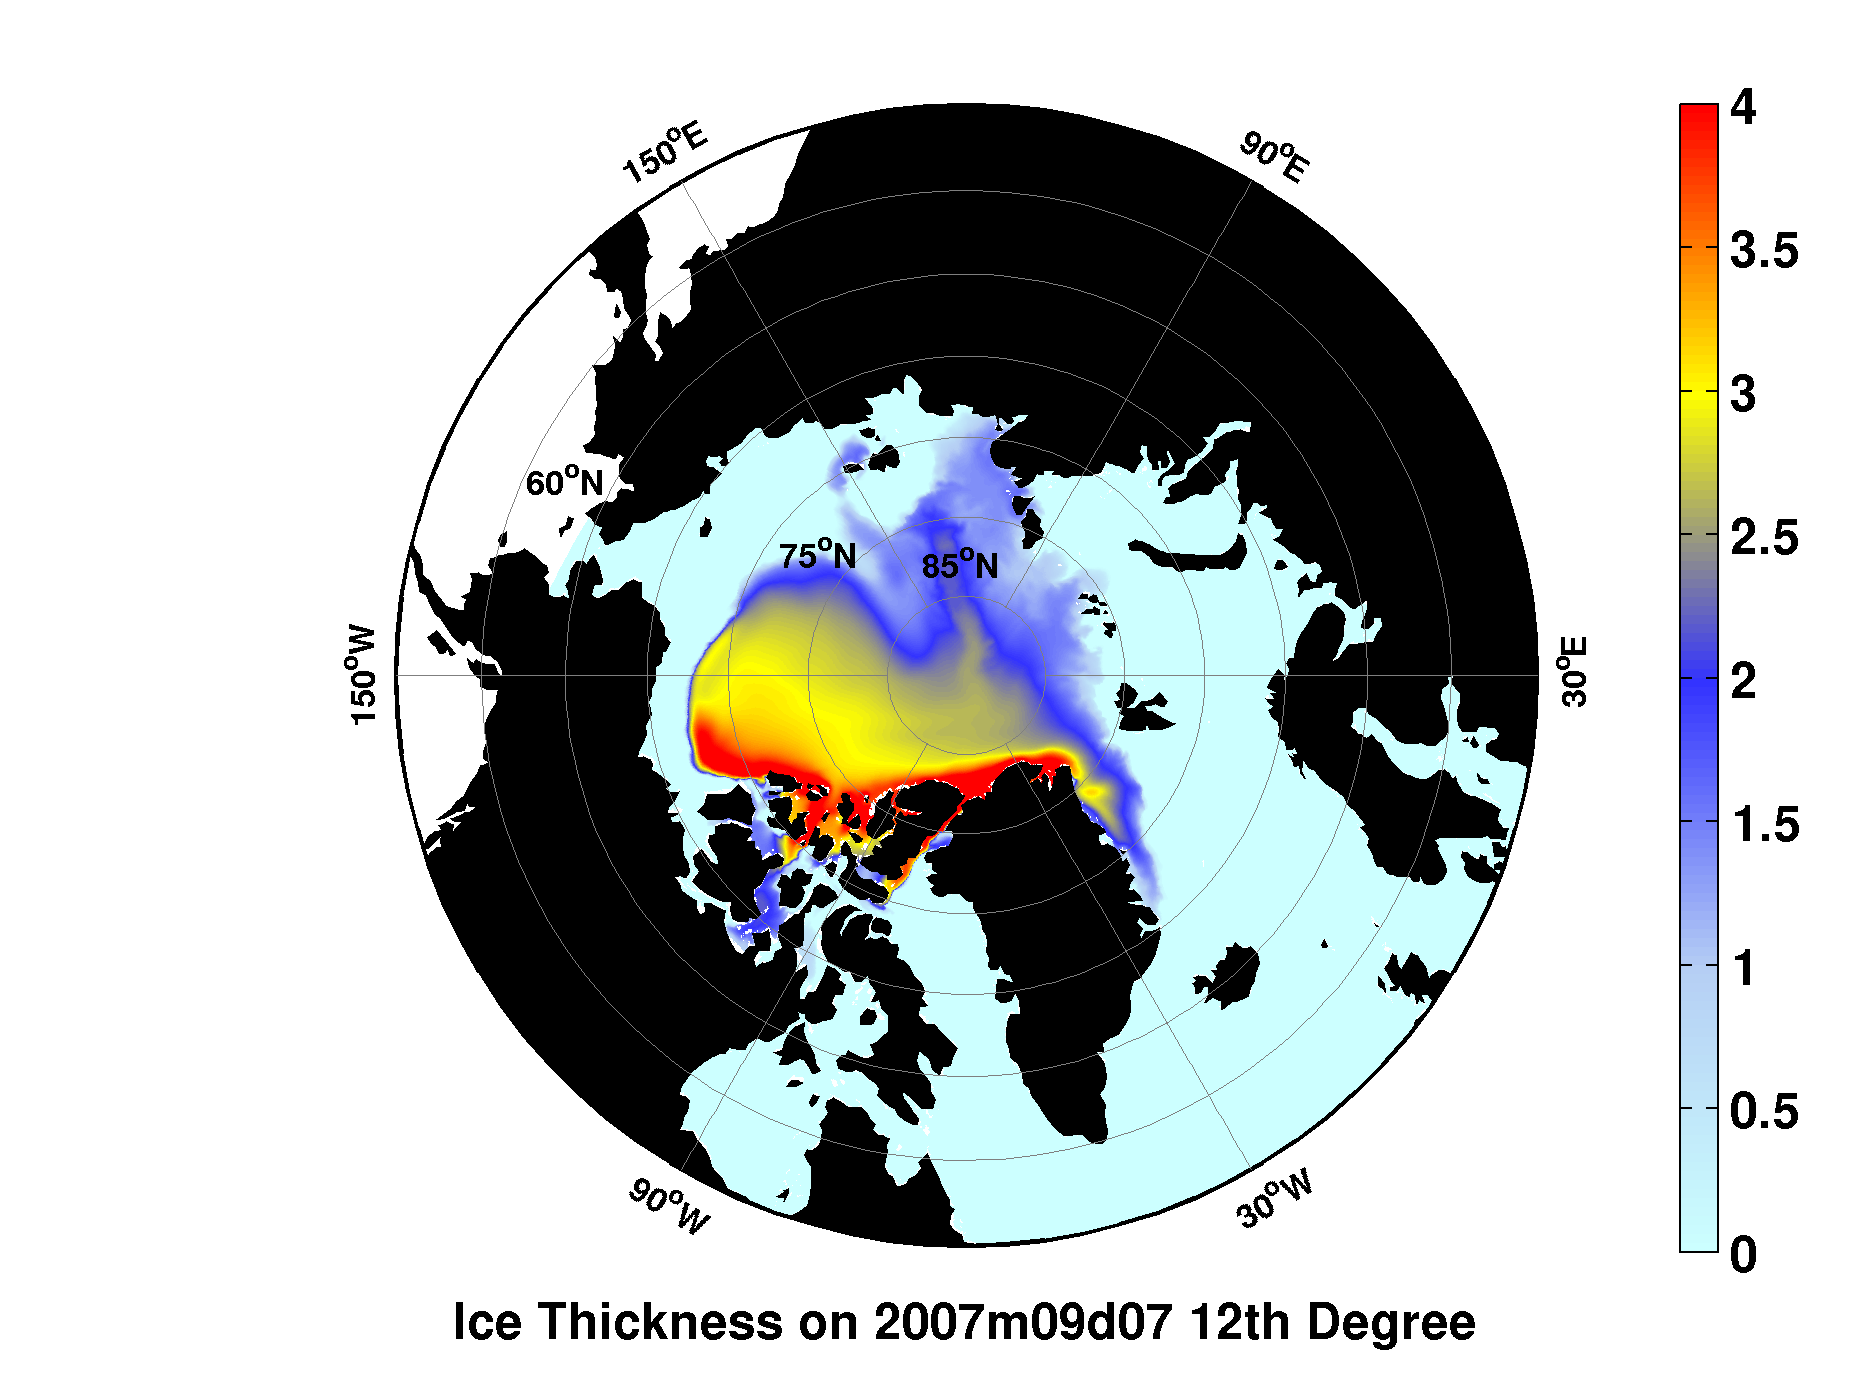
\includegraphics[width=\linewidth]{/home/jingfan/Desktop/Step1/3/Ice_Thickness_2007m09d07_12th_Degree.png}
\end{column}
\end{columns}

\end{frame}

\begin{frame}
\frametitle{Sea-Ice Thickness September 2007 Difference(ANHA12-ANHA4)}

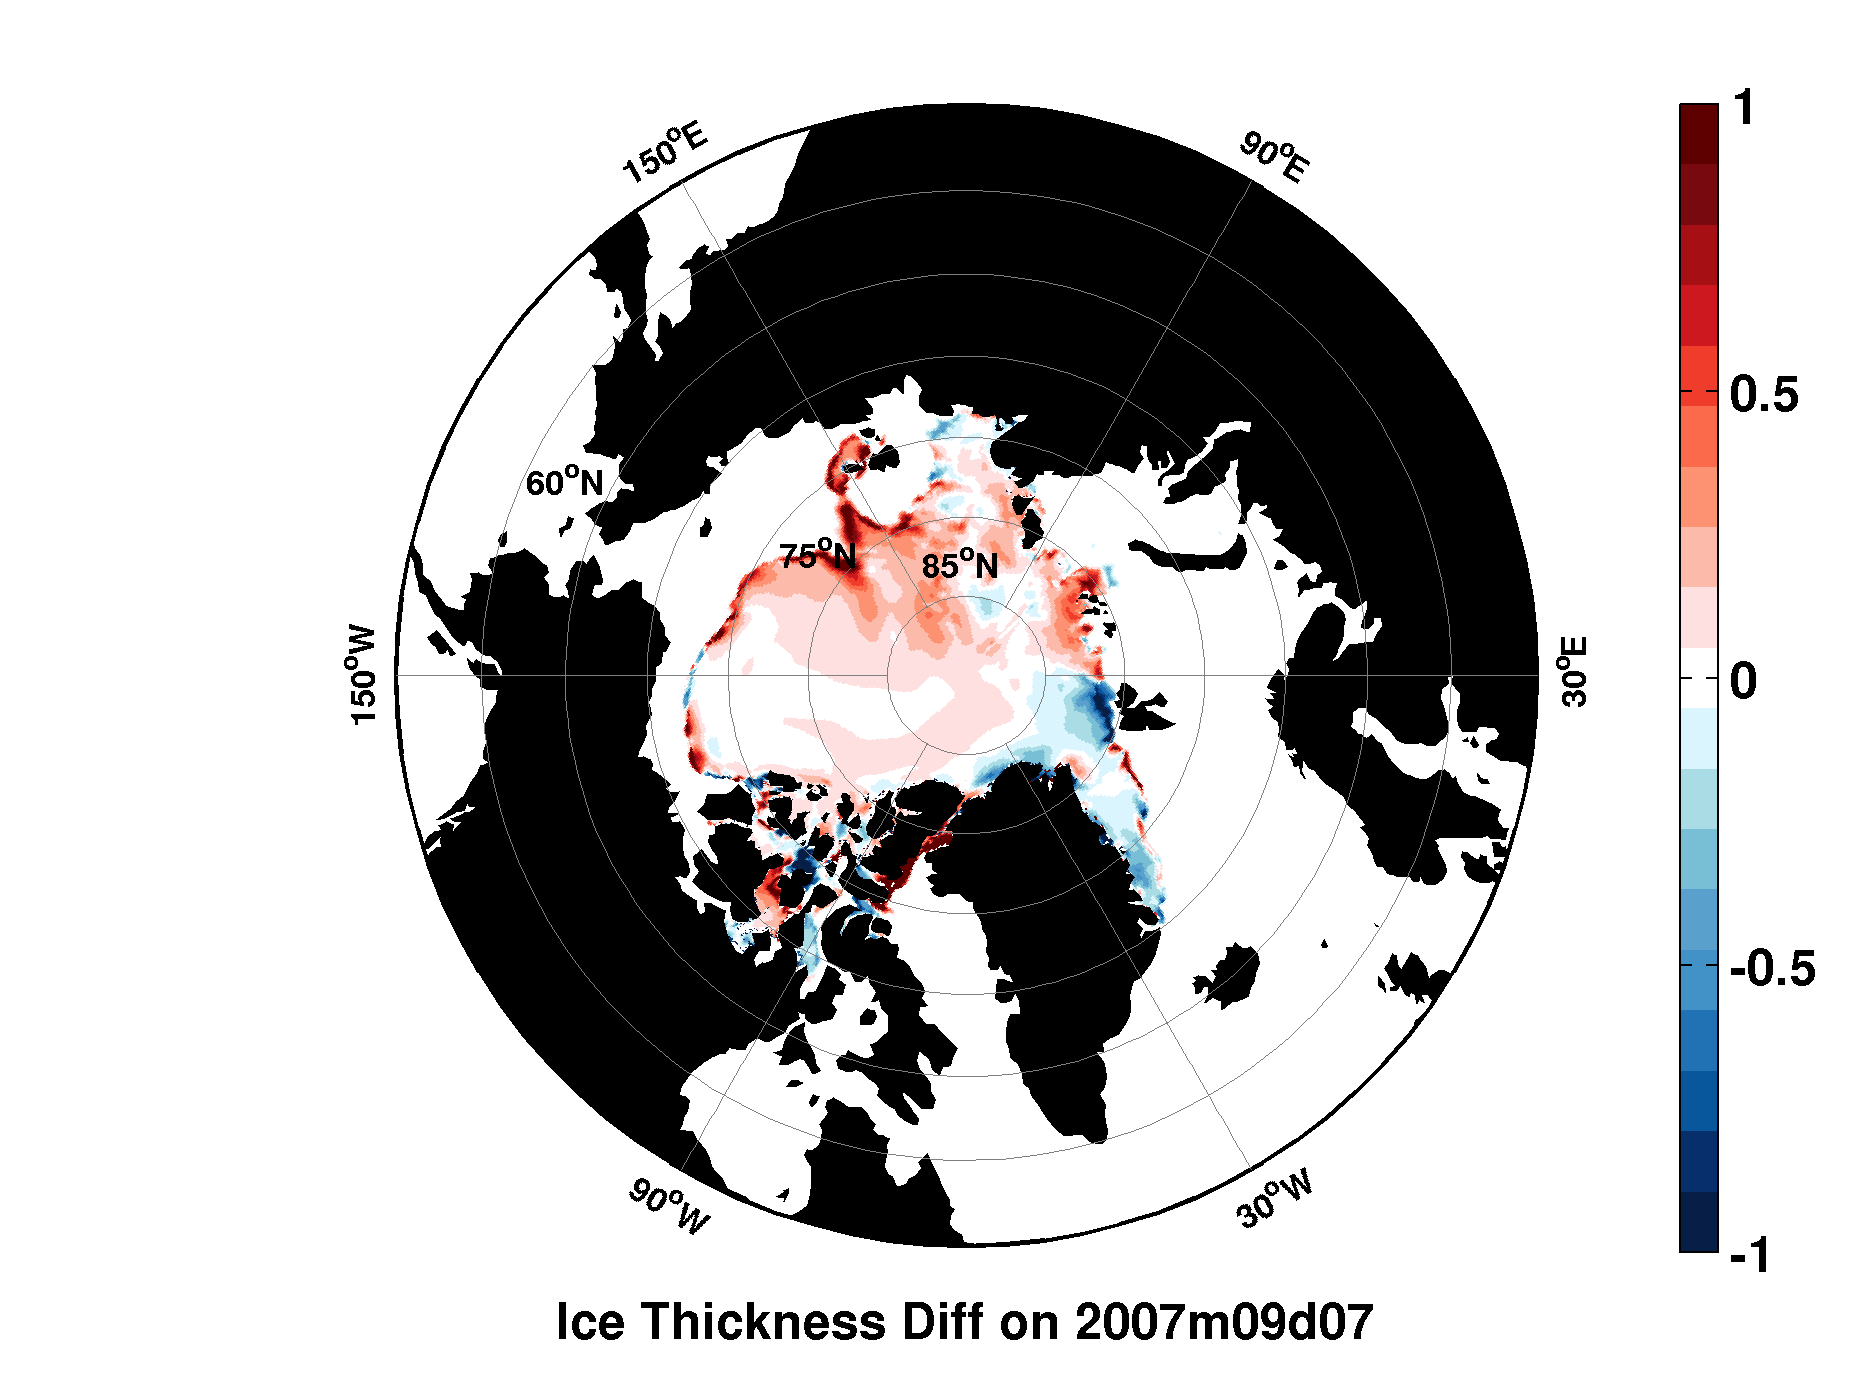
\includegraphics[width=0.9\linewidth]{/home/jingfan/Desktop/Step1/3/Ice_Thickness_Diff_2007m09d07.png}

\end{frame}

\begin{frame}
\frametitle{Sea-Ice Thickness September 2007}

\begin{columns}
\begin{column}[t]{0.5\linewidth}
\centering
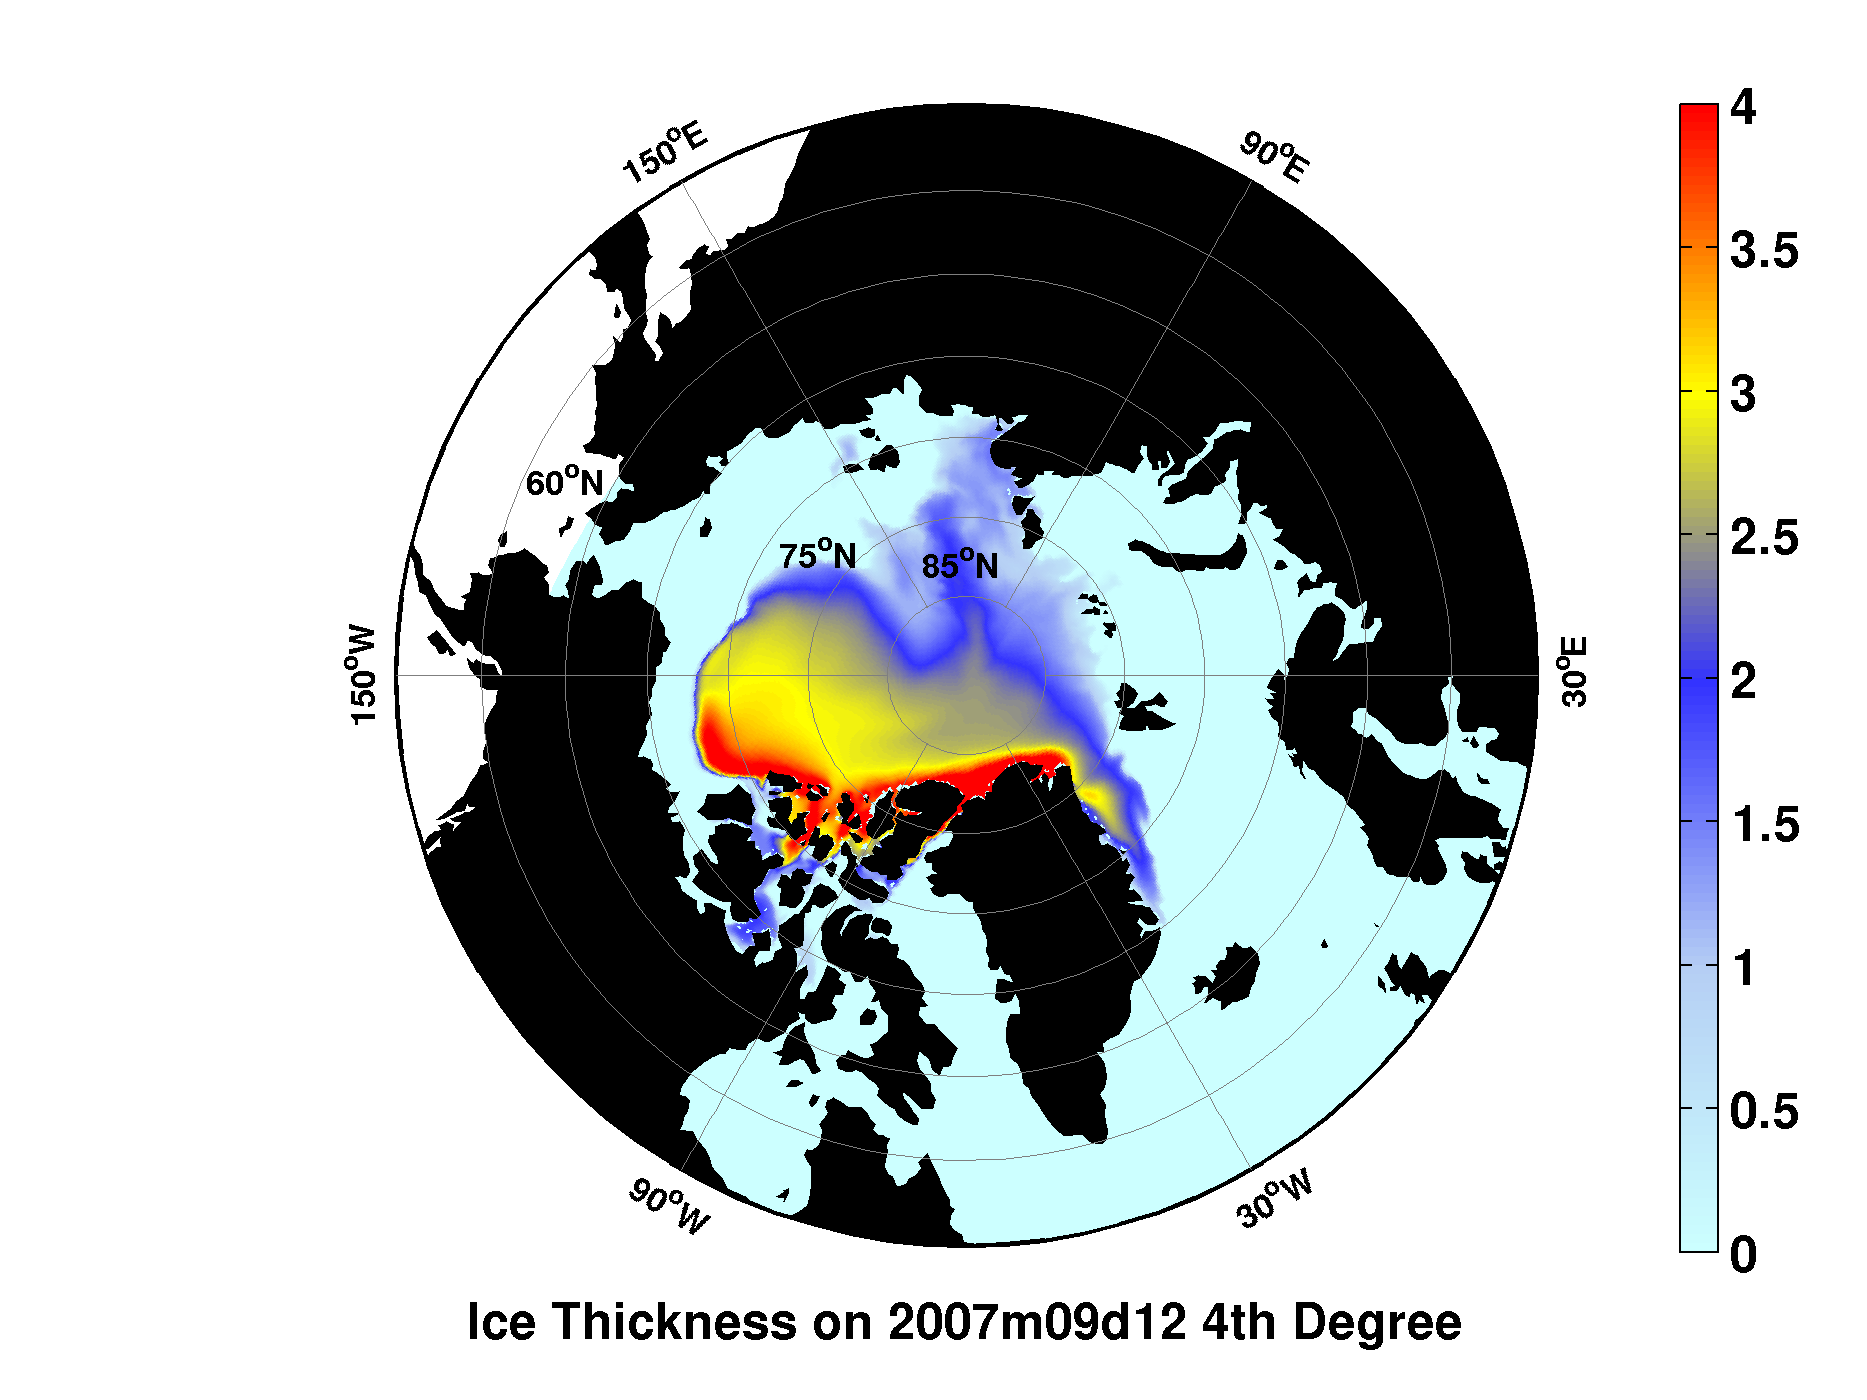
\includegraphics[width=\linewidth]{/home/jingfan/Desktop/Step1/3/Ice_Thickness_2007m09d12_4th_Degree.png}
\end{column}
\begin{column}[t]{0.5\linewidth}
\centering
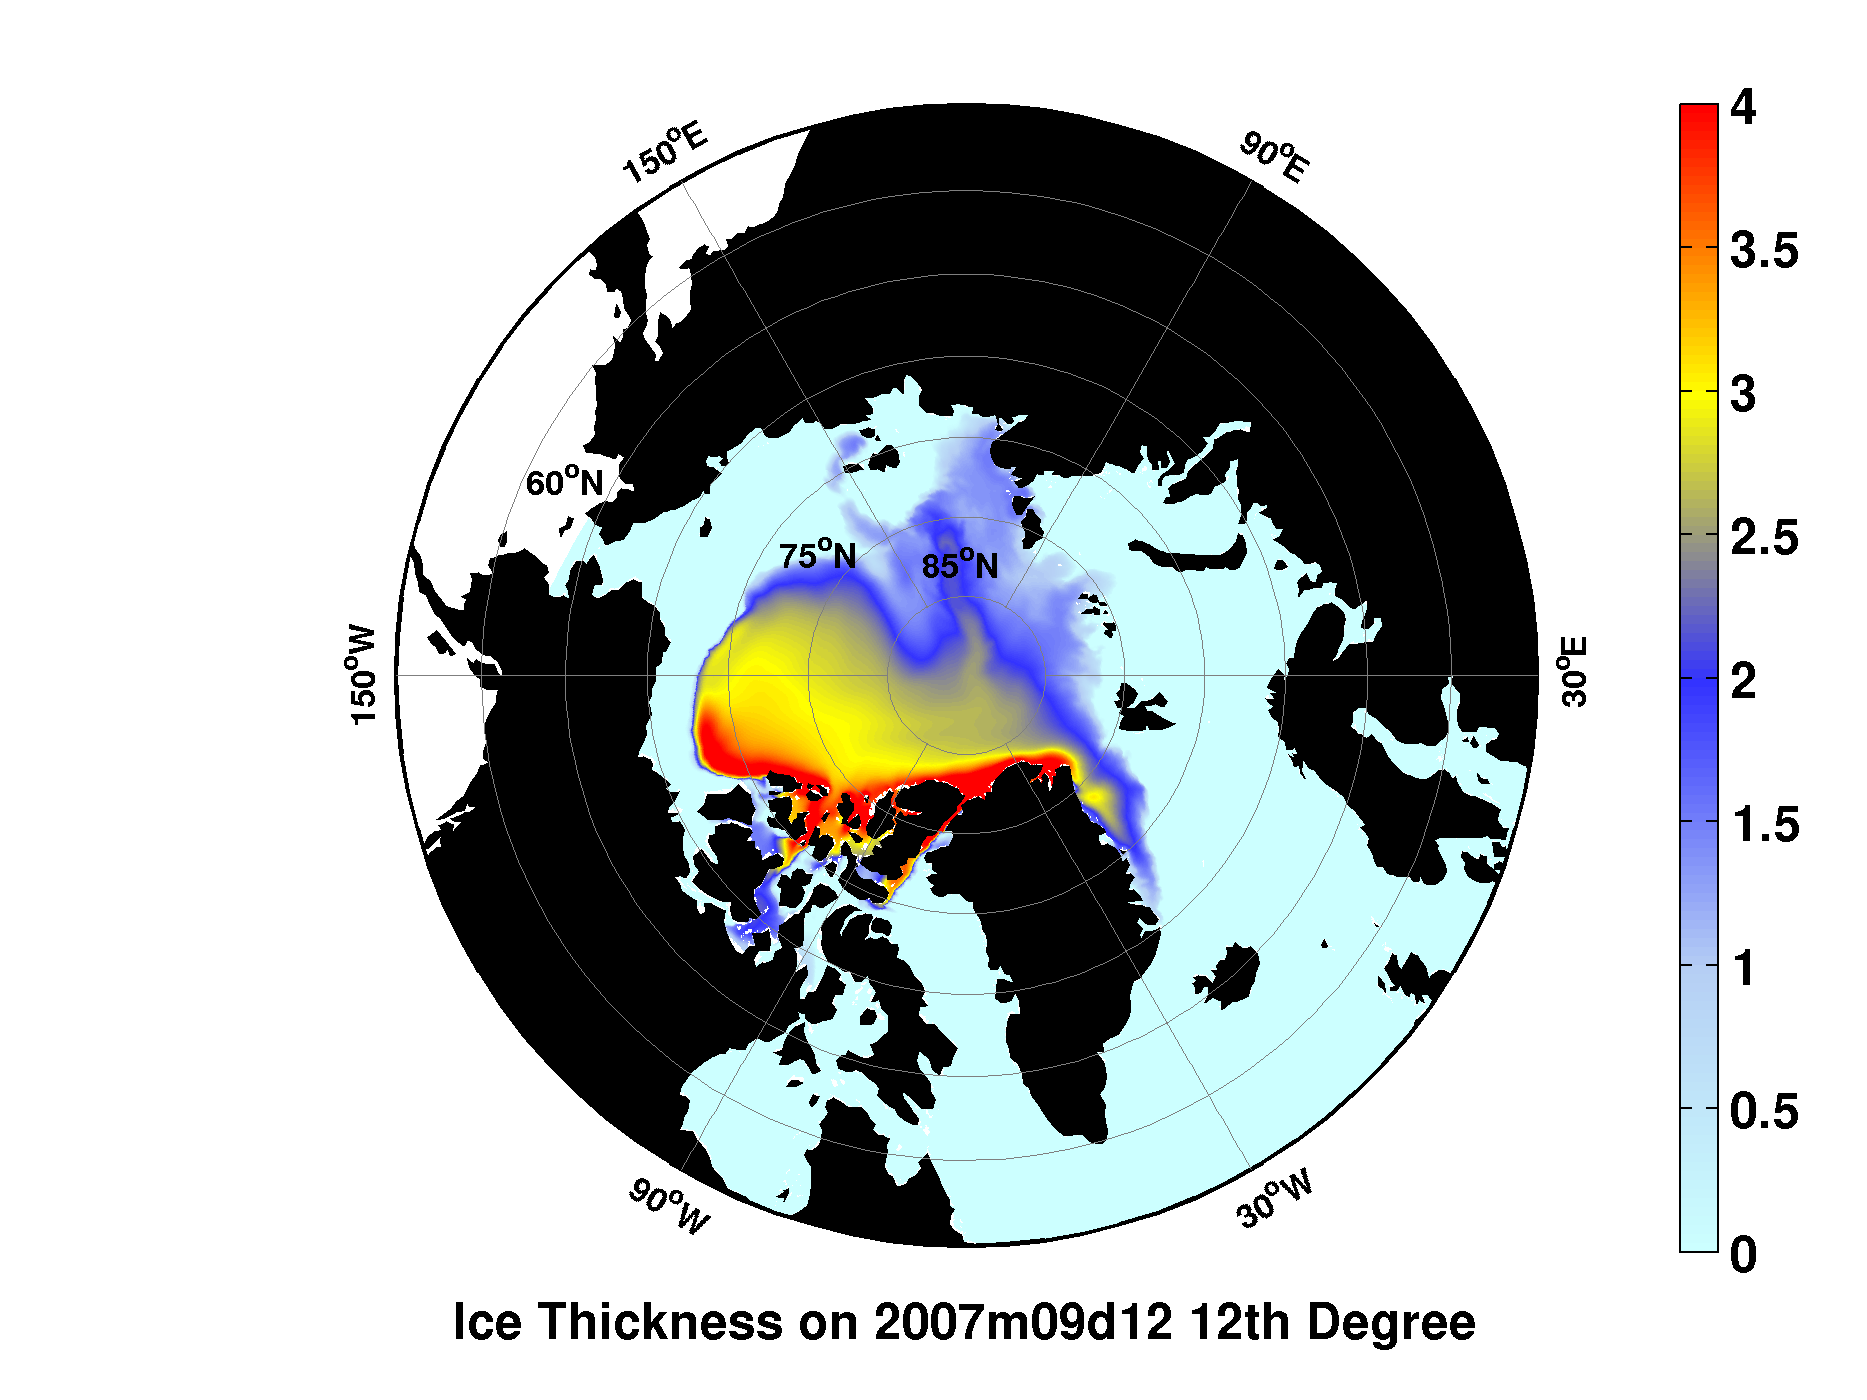
\includegraphics[width=\linewidth]{/home/jingfan/Desktop/Step1/3/Ice_Thickness_2007m09d12_12th_Degree.png}
\end{column}
\end{columns}

\end{frame}

\begin{frame}
\frametitle{Sea-Ice Thickness September 2007 Difference(ANHA12-ANHA4)}

\includegraphics[width=0.9\linewidth]{/home/jingfan/Desktop/Step1/3/Ice_Thickness_Diff_2007m09d12.png}

\end{frame}

\begin{frame}
\frametitle{Sea-Ice Thickness September 2007}

\begin{columns}
\begin{column}[t]{0.5\linewidth}
\centering
\includegraphics[width=\linewidth]{/home/jingfan/Desktop/Step1/3/Ice_Thickness_2007m09d17_4th_Degree.png}
\end{column}
\begin{column}[t]{0.5\linewidth}
\centering
\includegraphics[width=\linewidth]{/home/jingfan/Desktop/Step1/3/Ice_Thickness_2007m09d17_12th_Degree.png}
\end{column}
\end{columns}

\end{frame}

\begin{frame}
\frametitle{Sea-Ice Thickness September 2007 Difference(ANHA12-ANHA4)}

\includegraphics[width=0.9\linewidth]{/home/jingfan/Desktop/Step1/3/Ice_Thickness_Diff_2007m09d17.png}

\end{frame}

\begin{frame}
\frametitle{Sea-Ice Thickness September 2007}

\begin{columns}
\begin{column}[t]{0.5\linewidth}
\centering
\includegraphics[width=\linewidth]{/home/jingfan/Desktop/Step1/3/Ice_Thickness_2007m09d22_4th_Degree.png}
\end{column}
\begin{column}[t]{0.5\linewidth}
\centering
\includegraphics[width=\linewidth]{/home/jingfan/Desktop/Step1/3/Ice_Thickness_2007m09d22_12th_Degree.png}
\end{column}
\end{columns}

\end{frame}

\begin{frame}
\frametitle{Sea-Ice Thickness September 2007 Difference(ANHA12-ANHA4)}

\includegraphics[width=0.9\linewidth]{/home/jingfan/Desktop/Step1/3/Ice_Thickness_Diff_2007m09d22.png}

\end{frame}

\begin{frame}
\frametitle{Sea-Ice Thickness September 2007}

\begin{columns}
\begin{column}[t]{0.5\linewidth}
\centering
\includegraphics[width=\linewidth]{/home/jingfan/Desktop/Step1/3/Ice_Thickness_2007m09d27_4th_Degree.png}
\end{column}
\begin{column}[t]{0.5\linewidth}
\centering
\includegraphics[width=\linewidth]{/home/jingfan/Desktop/Step1/3/Ice_Thickness_2007m09d27_12th_Degree.png}
\end{column}
\end{columns}

\end{frame}

\begin{frame}
\frametitle{Sea-Ice Thickness September 2007 Difference(ANHA12-ANHA4)}

\includegraphics[width=0.9\linewidth]{/home/jingfan/Desktop/Step1/3/Ice_Thickness_Diff_2007m09d27.png}

\end{frame}

%%%%%%%%%%%%%%%%%%%%%%%%%%%%%%%%%%%%%%%%%%%%%%%%%%%%%%%%%%%%%%%
%% Sea-Ice Thickness Distribution
\section{Sea-Ice Thickness Distribution}
\begin{frame}
\frametitle{Sea-Ice Thickness Distribution}

I noticed that there are two types of methods to calculate the thickness distribution: 

\begin{itemize}

\item Directly calculate the mean ice thickness of a month based on the location and get the area of ice distributed in each bin
\item First, calculate the area distributed in each bin on each day of a month. Then get the mean distribution based on every single distribution.


\end{itemize}

The first attempt is an absolute one, while the second attempt is a relative one. I think the latter is more reasonable because it is not influenced by those thin ices which move drastically in a month-long time. Because of the movement of ice, thicker ice may be regarded as thinner one while calculating the mean in first method.

\end{frame}

\begin{frame}
\frametitle{Sea-Ice Thickness Distribution in March}

\begin{columns}
\begin{column}[t]{0.5\linewidth}
\centering
\includegraphics[width=\linewidth]{/home/jingfan/Desktop/Step1/4/Ice_Thickness_Distribution_2003-2008_March_4th_Degree.png}
\end{column}
\begin{column}[t]{0.5\linewidth}
\centering
\includegraphics[width=\linewidth]{/home/jingfan/Desktop/Step1/4/Ice_Thickness_Distribution_2003-2008_March_12th_Degree.png}
\end{column}
\end{columns}

\end{frame}

\begin{frame}
\frametitle{Sea-Ice Thickness Distribution Difference(ANHA12-ANHA4) in March}

\includegraphics[width=0.9\linewidth]{/home/jingfan/Desktop/Step1/4/Ice_Thickness_Distribution_Diff_2003-2008_March.png}

\end{frame}

\begin{frame}
\frametitle{Sea-Ice Thickness Distribution in September}

\begin{columns}
\begin{column}[t]{0.5\linewidth}
\centering
\includegraphics[width=\linewidth]{/home/jingfan/Desktop/Step1/4/Ice_Thickness_Distribution_2003-2008_September_4th_Degree.png}
\end{column}
\begin{column}[t]{0.5\linewidth}
\centering
\includegraphics[width=\linewidth]{/home/jingfan/Desktop/Step1/4/Ice_Thickness_Distribution_2003-2008_September_12th_Degree.png}
\end{column}
\end{columns}

\end{frame}

\begin{frame}
\frametitle{Sea-Ice Thickness Distribution Difference(ANHA12-ANHA4) in September}

\includegraphics[width=0.9\linewidth]{/home/jingfan/Desktop/Step1/4/Ice_Thickness_Distribution_Diff_2003-2008_September.png}

\end{frame}

\end{document}
